\makeatletter
\def\input@path{{./apqdesign}}
\makeatother

%Ab Hier kommen die Einstellungen für das NEUE APQ-TUD_Design!!!
\documentclass[
class=book,
accentcolor=1b,
custommargins=geometry,
fontsize=11pt,
thesis={type=Versuchsanleitung},
ruledheaders=all,
headline=false,
instbox=false,
marginpar=false,
title=small,
ignore-missing-data=true,
twoside=false,
logofile=apqdesign/tuda_logo.pdf,
pdfa=false % Problem mit Paket pdfx
]{apqpub} 

% % % % % % % %
%Pakete
\usepackage{cancel}
\usepackage{float}
\usepackage{subfig}
\usepackage{amsmath,amsthm,amssymb,dsfont}
\usepackage{mathtools}
\usepackage{mathrsfs}
\usepackage{enumerate}
\usepackage{enumitem}
\usepackage{isotope}
\usepackage[ngerman]{babel}
\usepackage[utf8]{inputenc}
\usepackage{nicefrac}
\usepackage{upgreek}
\usepackage[section]{placeins}
\usepackage{braket}


\usepackage[backend=bibtex, sorting=none, style=numeric-comp, defernumbers]{biblatex}
\addbibresource{Literatur}

%\usepackage{multibib}
%\newcites{q}{Quellen}
%\newcites{erg}{Ergänzende Literatur}
%\newcites{wes}{Wesentliche Literatur}

\newtheorem{satz}{Satz}[section]
\newtheorem{lemma}[satz]{Lemma}
\newtheorem{kor}[satz]{Korollar}
\newtheorem{prop}[satz]{Proposition}
\newtheorem{frage}[satz]{Frage}

\newtheorem{defi}[satz]{Definition}

\newtheorem{bsp}[satz]{Beispiel}
\newtheorem{bem}[satz]{Bemerkung}
\newtheorem{beob}[satz]{Beobachtung}

\usepackage{siunitx}
\sisetup{
  locale = DE ,
  per-mode = fraction,
%  per-mode = symbol,
  math-micro = \upmu,
  text-micro = µ,
  separate-uncertainty = false,
}

\usepackage{geometry}
\geometry{
	reset,
	a4paper,
	top=20mm,
	bottom=25mm,
	inner=31mm,%7mm Bindekorrektur sind jetzt
	outer=24mm,%der neue Standard im APQ-Design!
	includefoot,
	includehead,
	footskip=10mm,
	nomarginpar
}

\usepackage{hyperref} % Immer als letztes laden
\def\UrlFont{\normalfont}
% % % % % % % %
%Weitere Änderungen
\DeclareOldFontCommand{\bf}{\normalfont\bfseries}{\mathbf}
%\renewcommand{\it}{\textit}
\RedeclareSectionCommand[afterskip=\baselineskip]{chapter}
\newcommand\todo[1]{\textcolor{red}{#1}}
\parindent 0pt
\addtokomafont{caption}{\rmfamily\small}
\addtokomafont{captionlabel}{\accentfont}



\addTitleBoxLogo*{\makebox[\linewidth][l]{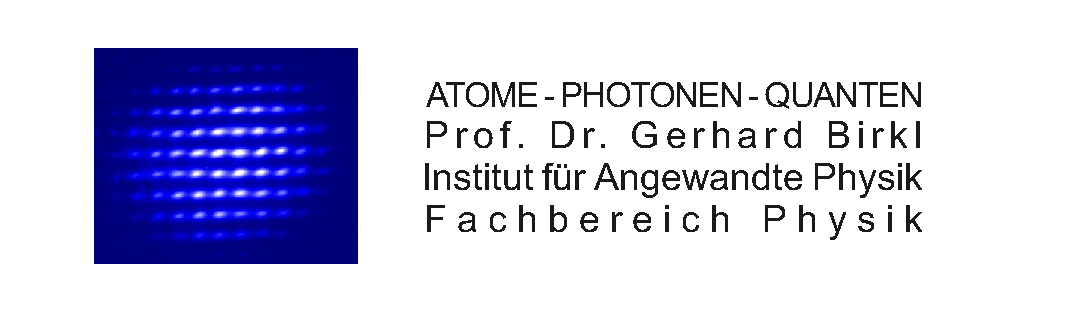
\includegraphics[width=55mm]{titel_apq-logo_1.pdf}}}

\graphicspath{{C:/Users/Max_Mustermann/Uni/Master/Masterarbeit/Results/}}%Möglichkeit einen generischen Pfad zu Abbildungen anzugeben.

%\lowertitleback{Textblock auf der Rückseite des Titelblattes. Enthält in der Regel Informationen über das Titelbild.}

\begin{document}
\renewcommand*{\figurename}{Abb.}
%\renewcommand*{\figurename}{Fig.} %Für englische Dokumente auskommentieren
\renewcommand*{\tablename}{Tab.}
	\titleimage{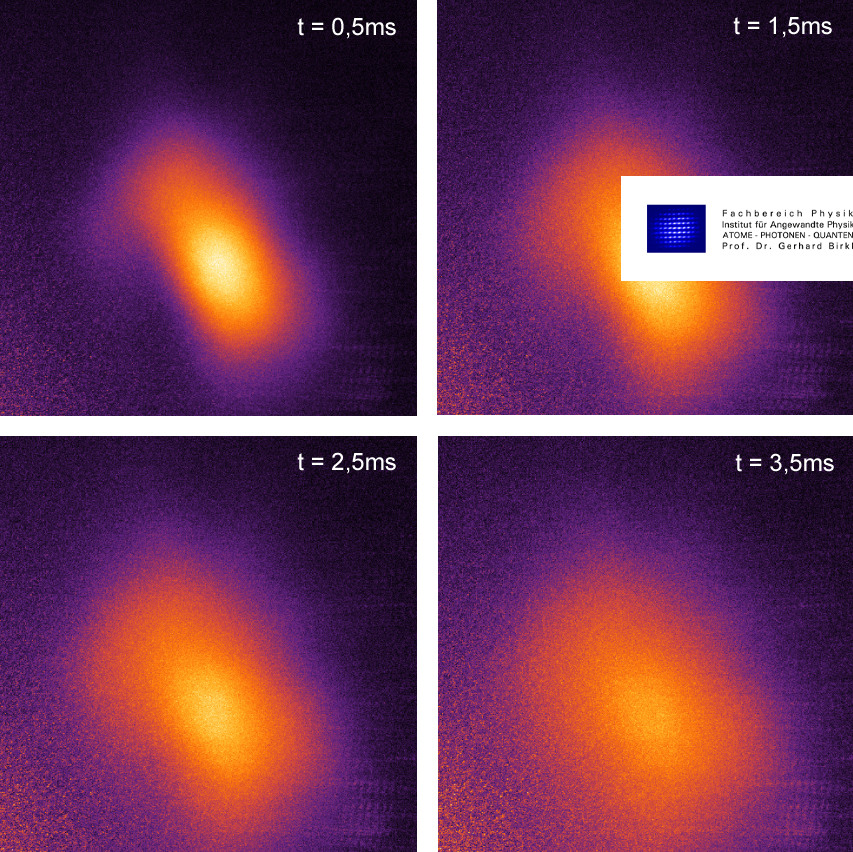
\includegraphics[width=\textwidth]{Bilder/g.jpg}}
	
	%%% Problem mit pdfx-Paket Start
	%\Metadata{
	%	title= Titel der Thesis, %% TUDaThesis -- Template für Abschlussarbeiten im CD der TU Darmstadt,
	%	author=Max Mustermann
	%}
	%%% Problem mit pdfx-Paket Ende
	
	%%%% Für den Titel sind 3 Zeilen vorgesehen.
	%%%% Hat der Titel nur zwei Zeilen, ist ein Zeillenumbruch (\\) einzufügen, um den Titel oben bündig zu positionieren
	%%%% Ist der Titel einzeilig sind zwei Freizeilen (\\ \ \\) anzuhängen.
	%%%% Ludwig Lind 03.02.2021
	\title{Fortgeschrittenenpraktikum \\ Abteilung A \\ 4.18 Mikro- und Fourieroptik}
	\subtitle{Micro and Fourier Optics}
	%\author[Max Mustermann]{Max Mustermann}%optionales Argument ist die Signatur,
	%\birthplace{Geburtsort}%Geburtsort, bei Dissertationen zwingend notwendig
	%\reviewer{Prof. Dr. Gerhard Birkl \and 2ter Gutachter}%Gutachter
	
	%Diese Felder erden untereinander auf der Titelseite platziert.
	%\department ist eine notwendige Angabe, siehe auch dem Abschnitt `Abweichung von den Vorgaben für die Titelseite'
	%\department{Fachbereich Physik} % Das Kürzel wird automatisch ersetzt und als Studienfach gewählt, siehe Liste der Kürzel im Dokument.
	%\institute{Institut für angewandte Physik}
	%\group{Atome-Photonen-Quanten}
	
	\submissiondate{\today}
	\examdate{\today} %\today
	\thesisdate{Stand Oktober 2023}
	
	%	\tuprints{urn=1234,printid=12345}
	%	\dedication{Für alle, die \TeX{} nutzen.}
	
	\maketitle
	\frontmatter
	
	%Füge in Abgaben mit twoside=false (z.B. Proposal) trotzdem titleback ein
%	\makeatletter
%	\if@twoside
%	\else%
%	\begingroup
%	\begin{minipage}[t]{\textwidth}
%		\@uppertitleback
%	\end{minipage}\par
%	\vfill
%	\begin{minipage}[b]{\textwidth}
%		\@lowertitleback
%	\end{minipage}\par
%	\@thanks\let\@thanks\@empty
%	\endgroup
%	\clearpage
%	\fi%
%	\makeatother
	 
%	\abstract{Inhaltliche Zusammenfassung der Thesis. Pflicht bei Masterarbeiten.}
	\tableofcontents
	
	\mainmatter
	\setcounter{page}{1}
	
	
	
	
\section{Warnhinweise und Spielregeln}

Die folgenden Warnhinweise dienen der eigenen Sicherheit und sollten daher unbedingt beachtet werden.

\begin{itemize}
	\item Während der gesamten Versuchsdurchführung ist eine geeignete Laserschutzbrille zu tragen!
	
	\item Achtung, Laserlicht! Die Laser haben zusammen überlagert etwa eine Gesamtleistung von 15mW, was bei
	einer Wellenlänge von 780nm ausreicht, um die menschliche Netzhaut nachhaltig zu schädigen. Beim Justieren
	darf daher kein Schmuck getragen werden und die Augen dürfen sich nie auf Strahlhöhe befinden.
	Es sind unbedingt die Richtlinien zum Laserschutz auf der letzten Seite dieser Anleitung zu beachten.
	
	Weitere Informationen sind online verfügbar:
	
	\url{www.iap.tu-darmstadt.de/lto/lp/laserschutz/lss_frames.html}
	
	\item Achtung, Hochspannung! Die Ionen-Getter-Pumpe wird mit einer Hochspannung von 7kV betrieben. Die
	Pumpe und das Hochspannungskabel sollten daher mit dem nötigen Respekt behandelt werden.
	
	\item Achtung, Magnetfelder! Von der Ionen-Getter-Pumpe gehen hohe Magnetfelder aus. Die Warnhinweise an
	der Pumpe sind daher unbedingt zu beachten.
\end{itemize}

Zu den Spielregeln.

\begin{itemize}
	\item Beide Praktikumspartner müssen gleichwertig und zu allen Themen auf den Versuch vorbereitet sein.
	
	\item Weitere Informationen können \url{http://www.fkp.tu-darmstadt.de/media/fachbereich_physik/phys_studium/phys_studium_bachelor/phys_studium_bsc_praktika/fpspielregeln.pdf} entnommen werden.
\end{itemize}

\section{Einleitung}

Betrachtet man die Themen der aktuellen Grundlagenforschung, so erkennt man, dass ein besonderer Fokus auf
Präzisionsmessungen mit ultra-kalten Atomen gerichtet ist. Zu diesen Experimenten zählen zum Beispiel die Untersuchung von kalten Stößen, die Realisierung von Atomuhren sowie die Quanteninformationsverarbeitung und
die Erzeugung eines Bose-Einstein-Kondensats.\\
Das Kühlen bzw. Vorkühlen dieser Atome erfolgt dabei stets durch den Einsatz von Laserlicht. Eine spezielle Art
zum Kühlen und Fangen von neutralen Atomen ist die magneto-optische Falle (magneto-optical trap, MOT). In
diesem Praktikumsversuch soll eine MOT erzeugt und $^{85}$Rb gefangen werden. Ziel ist es zu messen wie kalt die
Atome in der MOT schließlich sind.\\
Die Falle besteht, wie ihr Name schon sagt, aus zwei wesentlichen Komponenten: der optischen und der magnetischen.\\
Während es sich bei der magnetischen Komponente um ein Quadrupolfeld handelt, besteht die optische Komponente
aus Laserlicht sehr genau definierter Frequenzen. Da die Wellenlänge des Lichts auf wenige Pikometer genau stabil
gehalten werden muss, ist die Stabilisierung der Laser eine wesentliche Voraussetzung zur Erzeugung einer MOT.
Daher teilt sich dieser Versuch in zwei Teile:\\
Im ersten Teil soll auf die beiden Diodenlaser sowie deren Stabilisierungen eingegangen werden. Im Versuch werden
zwei verschiedene Arten der Stabilisierung eingesetzt, die es einzustellen und zu vermessen gilt. Im zweiten
Teil des Versuchs wird eine MOT erzeugt und vermessen. Dabei sollen Daten zur Bestimmung der Laderate der
Falle und die Temperatur der gefangenen Atome ermittelt werden.\\
Zunächst wird ein kurzer Überblick über den gesamten Versuchsaufbau gegeben.\\ 
Bevor dies stattfindet sollen jedoch die benötigten \textbf{Voraussetzungen zur Versuchsteilnahme} und die Präsenzaufgaben spezifiziert werden. 

\newpage

\section{Aufgaben}

Die Aufgaben gliedern sich zum einen in die \textbf{Vorbereitungsaufgaben}, welche vor der Versuchsdurchführung zu Hause zu bearbeiten sind, die \textbf{Präsenzaufgaben}, welche am Tag der Versuchsdurchführung zu erledigen sind und die \textbf{Auswertungsaufgaben}, welche nach der Versuchsdurchführung wiederum zu Hause zu erledigen sind.\\

\textbf{Hinweis:} Bringen Sie zur Versuchsdurchführung einen  \textbf{USB-Stick} mit, um die während der Versuchsdurchführung gewonnenen Daten mitnehmen zu können.

\subsection{Vorbereitungsaufgaben}

Zur Vorbereitung auf den Versuch sind sich einerseits die in 1. bis 4. aufgelisteten Themen zu erarbeiten und andererseits ist sich mit den im Anschluss aufgeführten Fragen zu beschäftigen, sodass diese im Vorbereitungsgespräch am Versuchstag beantwortet werden können. 

\begin{enumerate}
	\item \textbf{Versuchsaufbau:} Übersicht über den gesamten Aufbau, Laserstabilisierung, MOT
	
	\item \textbf{wichtige Bauteile:} Akusto-Optischer Modulator (AOM), Verzögerungsplatten ($\lambda/2$-, $\lambda/4$-Platten), Polarisationsstrahlteilerwürfel (PST), Photodiode, Ionen-Getter-Pumpe, PID-Regler
	
	\item \textbf{Theorie Laserstabilisierung:} Diodenlaser mit externem Resonator, dopplerfreie Sättigungsspektroskopie, Offsetlock
	
	\item \textbf{Theorie MOT:} Dopplerkühlung, Energieniveaustruktur $^{85}$Rb, Quadrupolfeld, Sub-Dopplerkühlung   
\end{enumerate}

\textbf{Anmerkung:} Die Anleitung zum Versuch stellt eine Einführung in das Thema dar. Um die Vorbereitung zu erleichtern sind die unter 1. und 2. aufgeführten Punkte in der Anleitung in der zur Versuchsdurchführung hinreichenden Tiefe dargestellt. Hier muss keine zusätzliche Literatur zurate gezogen werden. Die unter 3. und 4. aufgeführten Themen werden hingegen lediglich andiskutiert und zu deren Verständnis ist es \textit{unerlässlich} zusätzliche Literatur durchzuarbeiten. Hierzu existiert eine \nameref{sec:LE}. Insbesondere zum Thema der Subdopplerkühlung sei auf Quelle (v) Seiten 218-226 hingewiesen.\\

\textbf{Fragen:}  

In den jeweiligen Abschnitten finden Sie Fragen, die Sie zur Vorbereitung beantworten sollen (Frage 4.1 bis 7.1 (siehe unten)). In \autoref{sec:FK} finden Sie zudem einen Fragenkatalog mit zusätzlichen fakultativen Fragen, welchen Sie zur Überprüfung Ihres Vorbereitungsstandes nutzen können.

\begin{itemize}
	\item \textbf{Frage 4.1:} Welchen Vorteil bietet es den Aufbau der MOT durch ein Glasfaserkabel von dem Aufbau der Laserstabilisierung zu trennen?
	
	\item \textbf{Frage 5.1:} Inwiefern ist die durch den AOM verursachte Frequenzverschiebung des Laserlichts in Bezug auf die Stabilisierung des Rückpump- und Kühllasers bzw. die an der MOT benötigte Frequenz relevant?
	
	\item \textbf{Frage 5.2:} Zu welchem Zweck werden die in den schematischen Skizzen zur Laserstabilisierung und der MOT eingezeichneten Verzögerungsplatten jeweils verwendet?
	
	\item \textbf{Frage 5.3:} Zu welchem Zweck werden die PST verwendet und warum kommen sie stets in Kombination mit einer $\lambda/2$-Platte vor?  
	
	\item \textbf{Frage 6.1:} Durch welche Größen/Faktoren werden die Laserfrequenzen beeinflusst? Welche dieser Faktoren sind gewollt beziehungsweise ungewollt und wie können diese beseitigt werden?
	
	\item \textbf{Frage 7.1:} Welche Elemente werden zur Erzeugung einer MOT benötigt? Wo wird das Licht in die drei Strahlen aufgeteilt? Wie verlaufen die Strahlen?
\end{itemize}

\newpage

\subsection{Präsenzaufgaben}

\begin{itemize}
	
	\item \textbf{Stabilisierung der Laser:} Zur Stabilisierung der Laser betrachten Sie zunächst das Spektroskopiesignal des Rückpumplasers und stabilisieren Sie diesen auf den F=2 nach F'=1 Übergang. Betrachten Sie dazu das Spektroskopiesignal des Rückpumplasers und das zugehörige Dispersionssignal. Nehmen sie beide Signale mit Hilfe des digitalen Oszilloskops und der zugehörigen Computersoftware auf.
	
	\item \textbf{Spektroskopie des Kühllasers:} Durch Verschieben der Rubidiumdampfzelle in den Strahlengang des Kühllasers können Sie eine Spektroskopie an diesem durchführen. Nehmen Sie dieses Signal ebenfalls mit Hilfe des digitalen Oszilloskops auf.
	
	\item \textbf{Ladephase der MOT:} Nehmen Sie eine Messreihe zur Untersuchung der Ladephase der MOT auf und teilen Sie diese dazu in geeignete Zeitabschnitte ein.
	
	\item \textbf{Temperatur in der MOT:} Nehmen Sie eine geeignete Messreihe zur Bestimmung der Temperatur in der MOT auf.
	
	\item \textbf{Temperatur nach der Melassenphase:} Nehmen Sie eine Messreihe zur Bestimmung der Temperatur nach der Melassenphase auf.
	
\end{itemize}

\subsection{Auswertungsaufgaben}

\begin{itemize}
	
	\item \textbf{Spektroskopie:} Stellen Sie die aufgenommenen Spektroskopiesignale des Rückpump- (inkl. Dispersionssignal) und Kühllasers graphisch dar und diskutieren Sie das Ergebnis.
	
	\item \textbf{Ladephase:} Betrachten Sie Ihre aufgenommene Messreihe zur Ladephase der MOT. Stellen Sie deren zeitlichen Verlauf dar und approximieren Sie diesen mit einer geeigneten Funktion. Beschreiben Sie das Ergebnis.\\
	(Zur Charakterisierung des Ladezustandes bietet es sich an, die Gesamtintensität der aufgenommenen Bilder zu betrachten - also die Summe über alle einzelnen Pixelwerte.)
	
	\item \textbf{Temperatur in der MOT:} Bestimmen Sie mit Hilfe Ihrer aufgenommenen Messreihe die Temperatur in der MOT. Dazu soll zunächst die mittlere Geschwindigkeit der Atome aus den gewonnenen Daten ermittelt werden. 
	
	\item \textbf{Temperatur nach der Melassenphase:} Bestimmen Sie analog zur Temperatur in der MOT nun die Temperatur nach der Melassenphase. Erklären Sie auftretende Abweichungen im Vergleich zu der Temperatur der Atome in der MOT.
\end{itemize}

\section{Literaturempfehlung}\label{sec:LE}

\begin{enumerate}[label=\roman*]
	\item D. Meschede. \textit{Optik, Licht und Laser}. Vieweg-Teubner, 2008.
	
	\item F. Pedrotti, L. Pedrotti, W. Bausch, and H. Schmidt. \textit{Optik für Ingenieure - Grundlagen (3. Auflage)}. Springer, 2005.
	
	\item W. Demtröder.\textit{Laserspektroskopie - Grundlagen und Techniken}. Springer 2007. Seiten 328 - 335
	
	\item H. Metcalf and P. van der Straten. \textit{Laser cooling and trapping}. Springer 2002. Kapitel 3; 4.1; 7; 8; 11.4
	
	\item W. D. Philips. \textit{Laser cooling and trapping of neutral altoms (Noble Lecture)}.  \url{http://www.nobelprize.org/nobel_prizes/physics/laureates/1997/phillips-lecture.html} Seiten 218 - 226
	
	
\end{enumerate}

\newpage

\section{Überblick über den Versuchsaufbau}

Ziel dieses Kapitels ist es, zunächst einen Überblick über den gesamten Versuchsaufbaus zu schaffen. Anschließend soll näher auf die beiden wesentlichen Teile, die Laserstabilisierung und die MOT eingegangen werden. Es empfiehlt sich dieses Kapitel als Lageplan ähnlich dem eines Reiseführers zu verstehen und diesen als Ausgangspunkt zur Beschäftigung mit den einzelnen ``Sehenswürdigkeiten'' zu verwenden.\\
~\\  
Der Gesamtversuchsaufbau besteht aus drei Hauptteilen (siehe Gesamtbild auf Seite 1), dem optischen Versuchsaufbau (rechts), dem Elektronikrack zur Experimentsteuerung (Mitte) und dem Computersystem zur Datenaufnahme (links). Diese Teile werden im Folgenden genauer vorgestellt.

\begin{figure}[htb!]
	\centering
	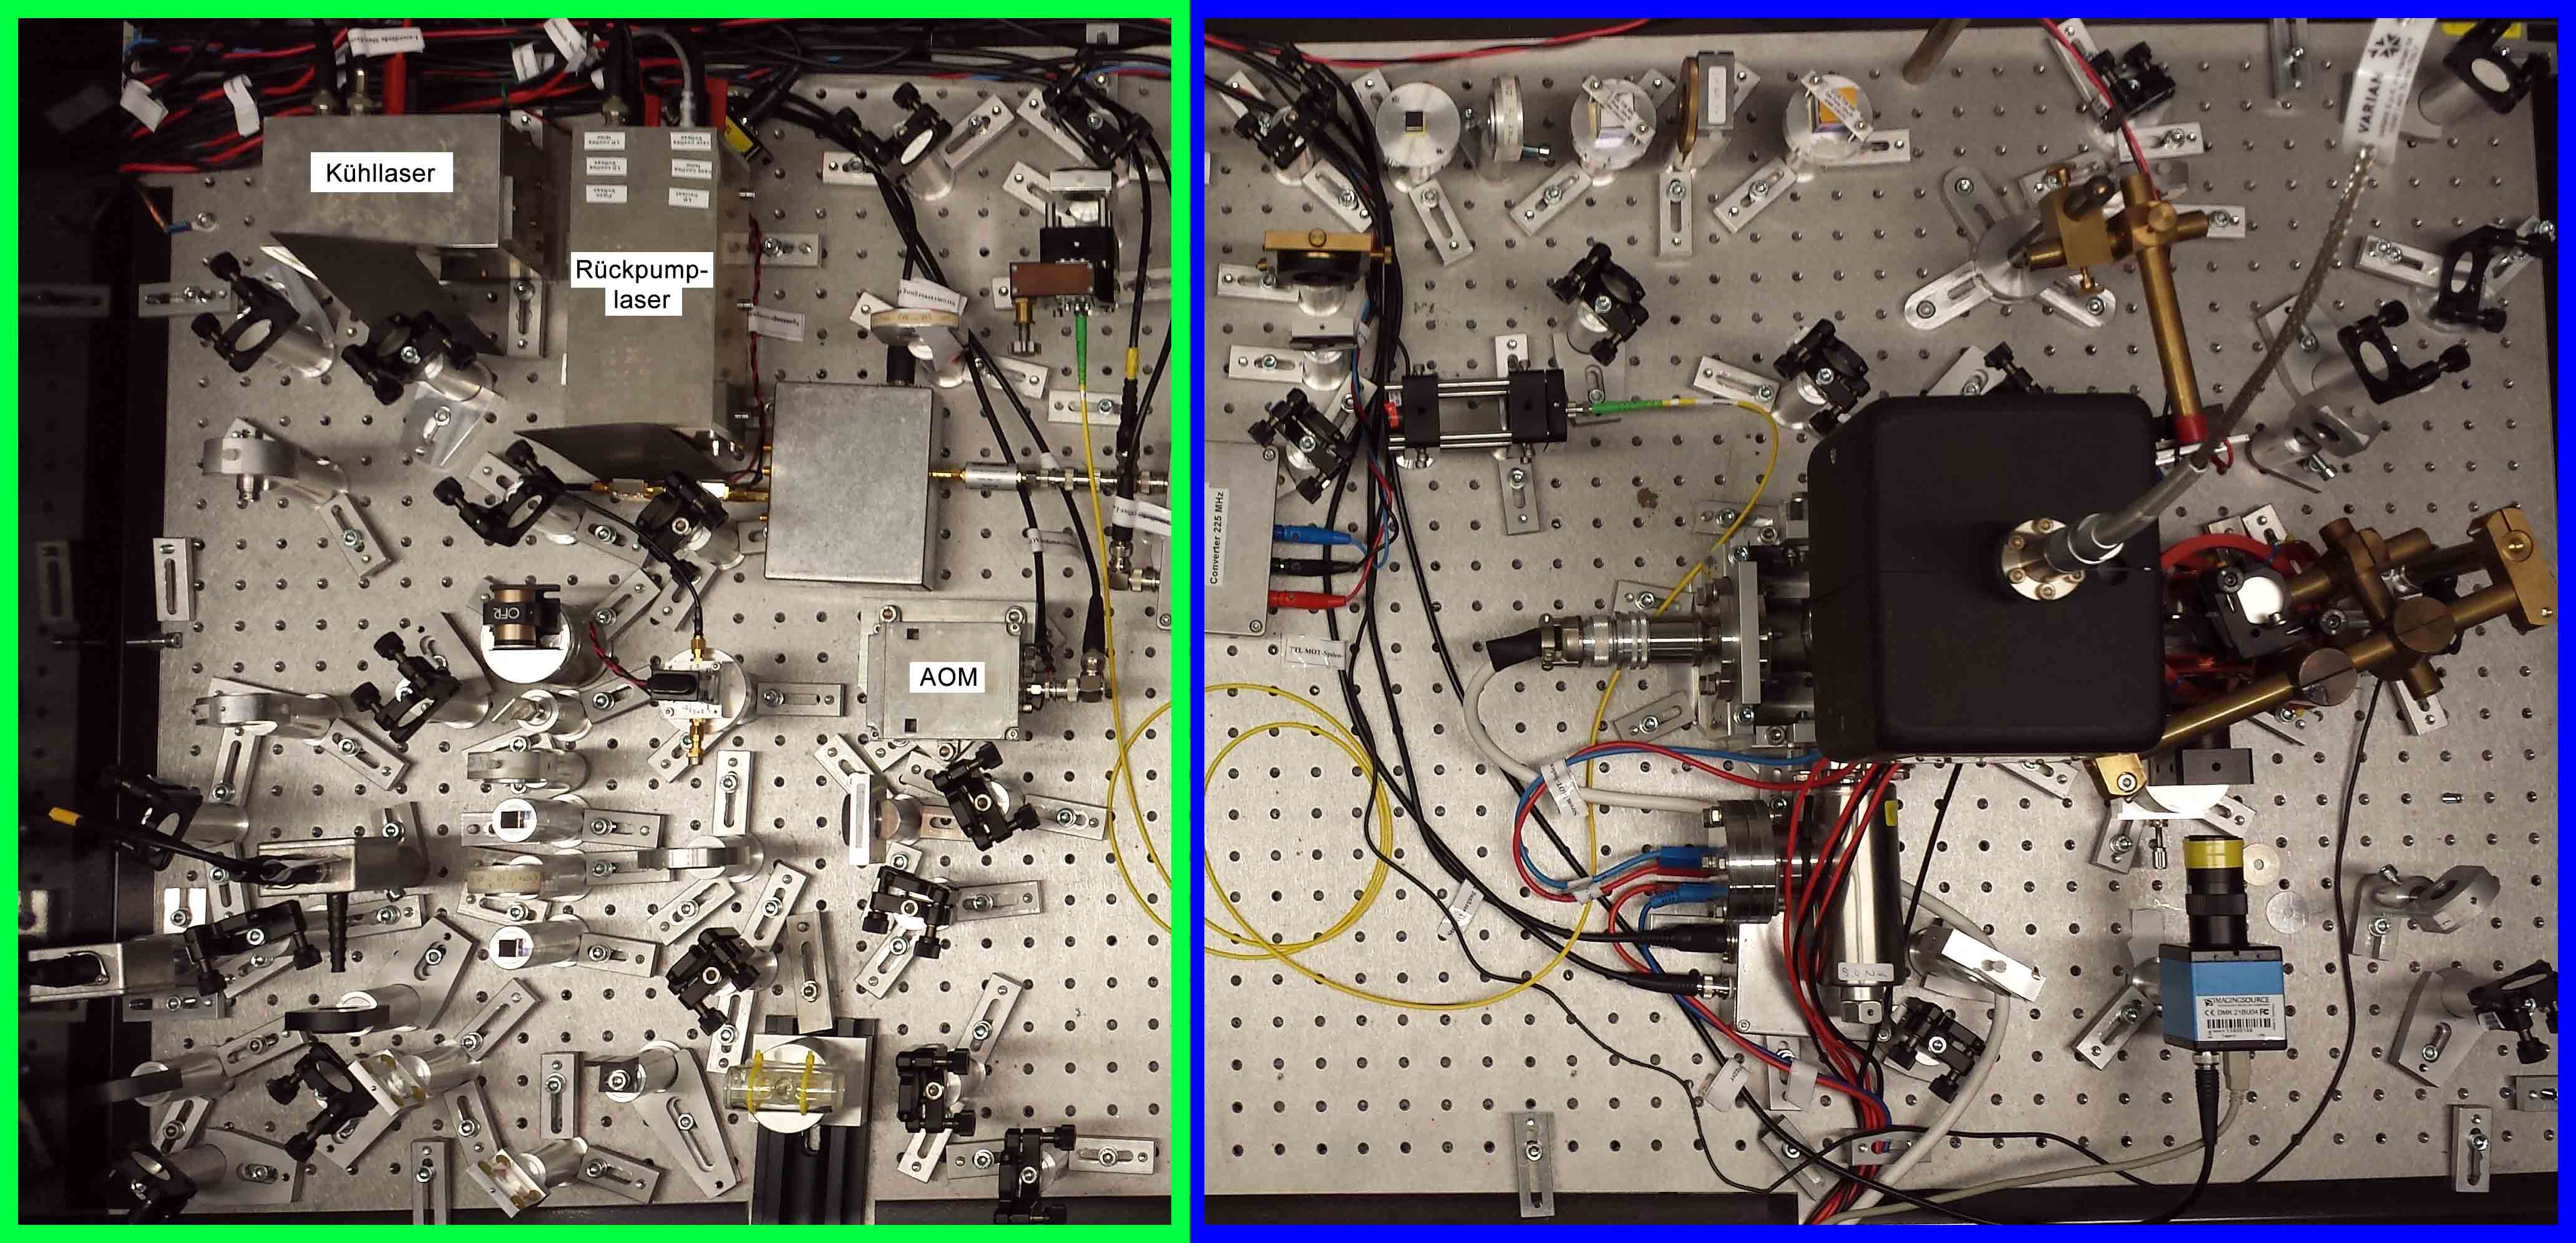
\includegraphics[width=480px]{Bilder/GUE3.jpg}
	\caption{Übersicht über den Versuchsaufbau}
	\label{fig:GUE}
\end{figure}

In \autoref{fig:GUE} ist auf der linken Seite (\textcolor{green}{grün} umrandet) der Aufbau zur Laserstabilisierung und auf der rechten Seite (\textcolor{blue}{blau} umrandet) der Aufbau zur MOT zu erkennen.

\begin{figure}[htb!]
	\centering
	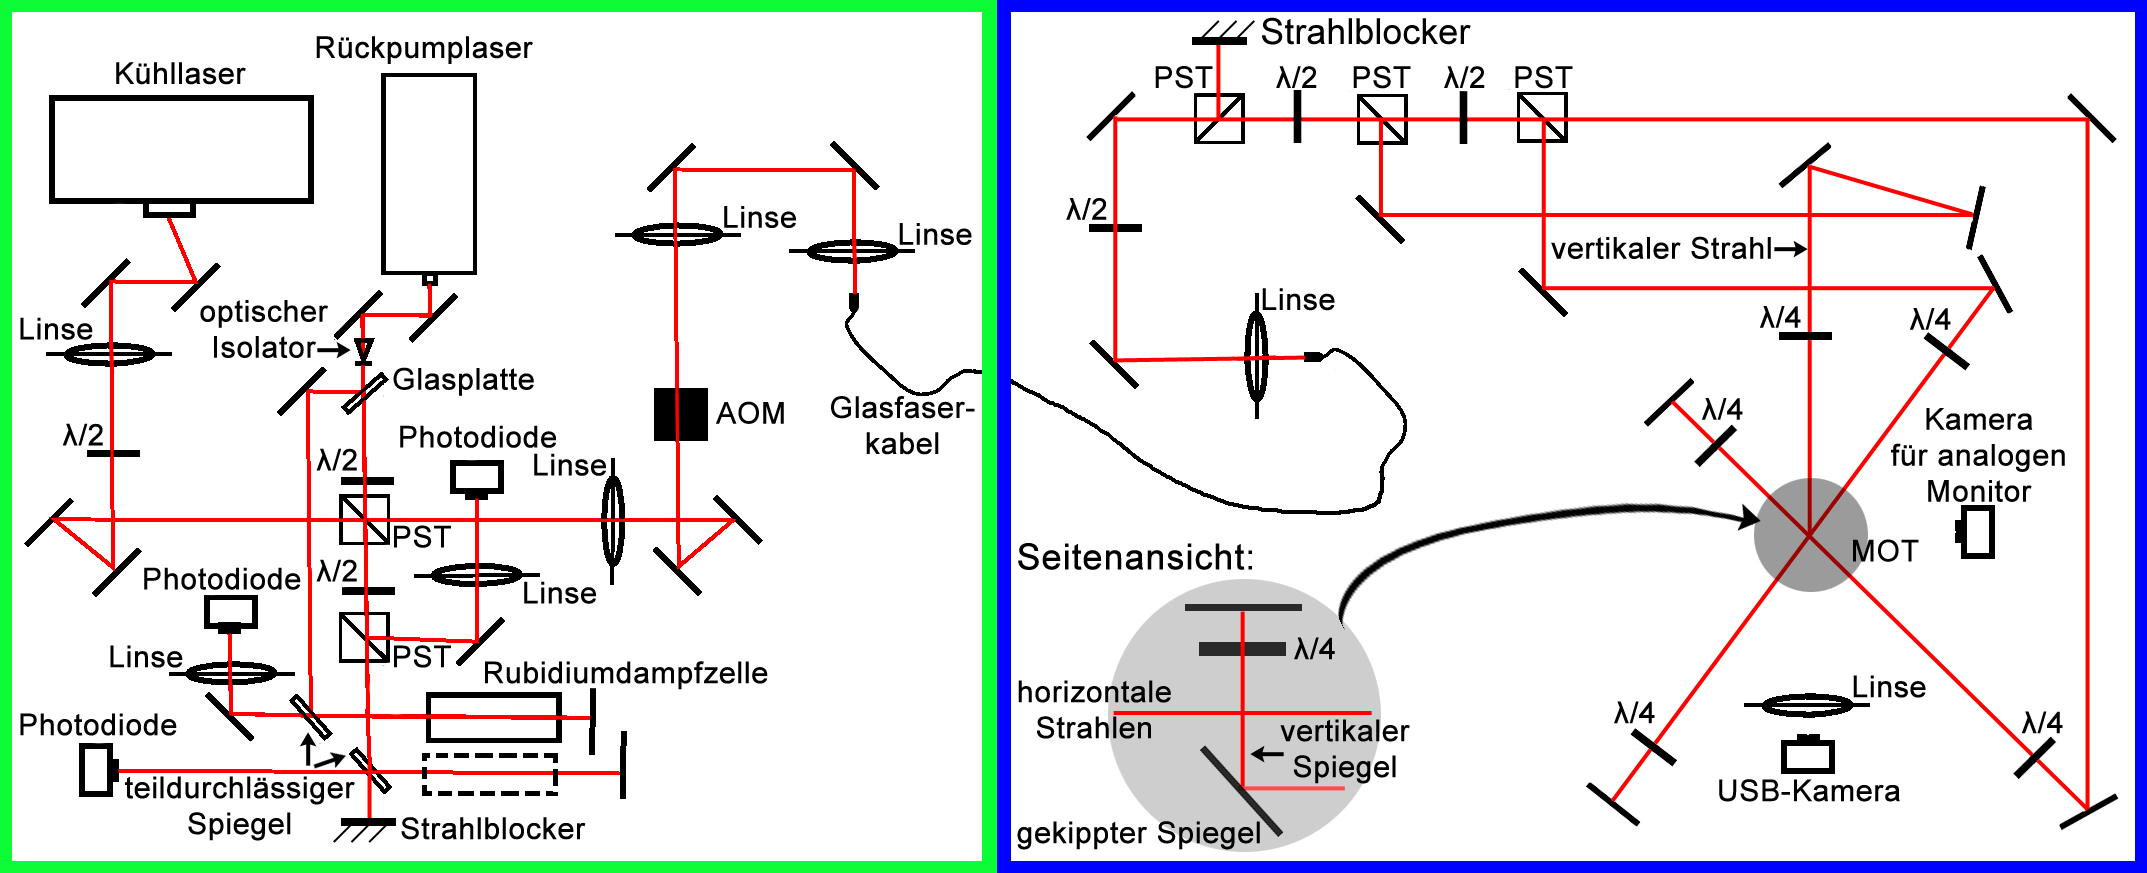
\includegraphics[width=480px]{Bilder/TZ2.jpg}
	\caption{Technische Skizze des Aufbaus}
	\label{fig:TZ}
\end{figure} 

Im Folgenden soll ein Überblick über den Aufbau gegeben werden. Betrachten Sie dazu auch die technischen Zeichnungen des Aufbaus zur Laserstabilisierung und zur Strahlführung der MOT (in \autoref{fig:TZ} ebenfalls \textcolor{green}{grün} und \textcolor{blue}{blau} markiert) und vergleichen Sie diese mit den Bildern des Aufbaus.\\
In \autoref{fig:Rack} ist der nicht minder wichtige Aufbau der Experimentensteuerung dargestellt, welcher ebenso in die Betrachtung mit eingeschlossen werden sollte.\\

\begin{figure}[htb!]
	\centering
	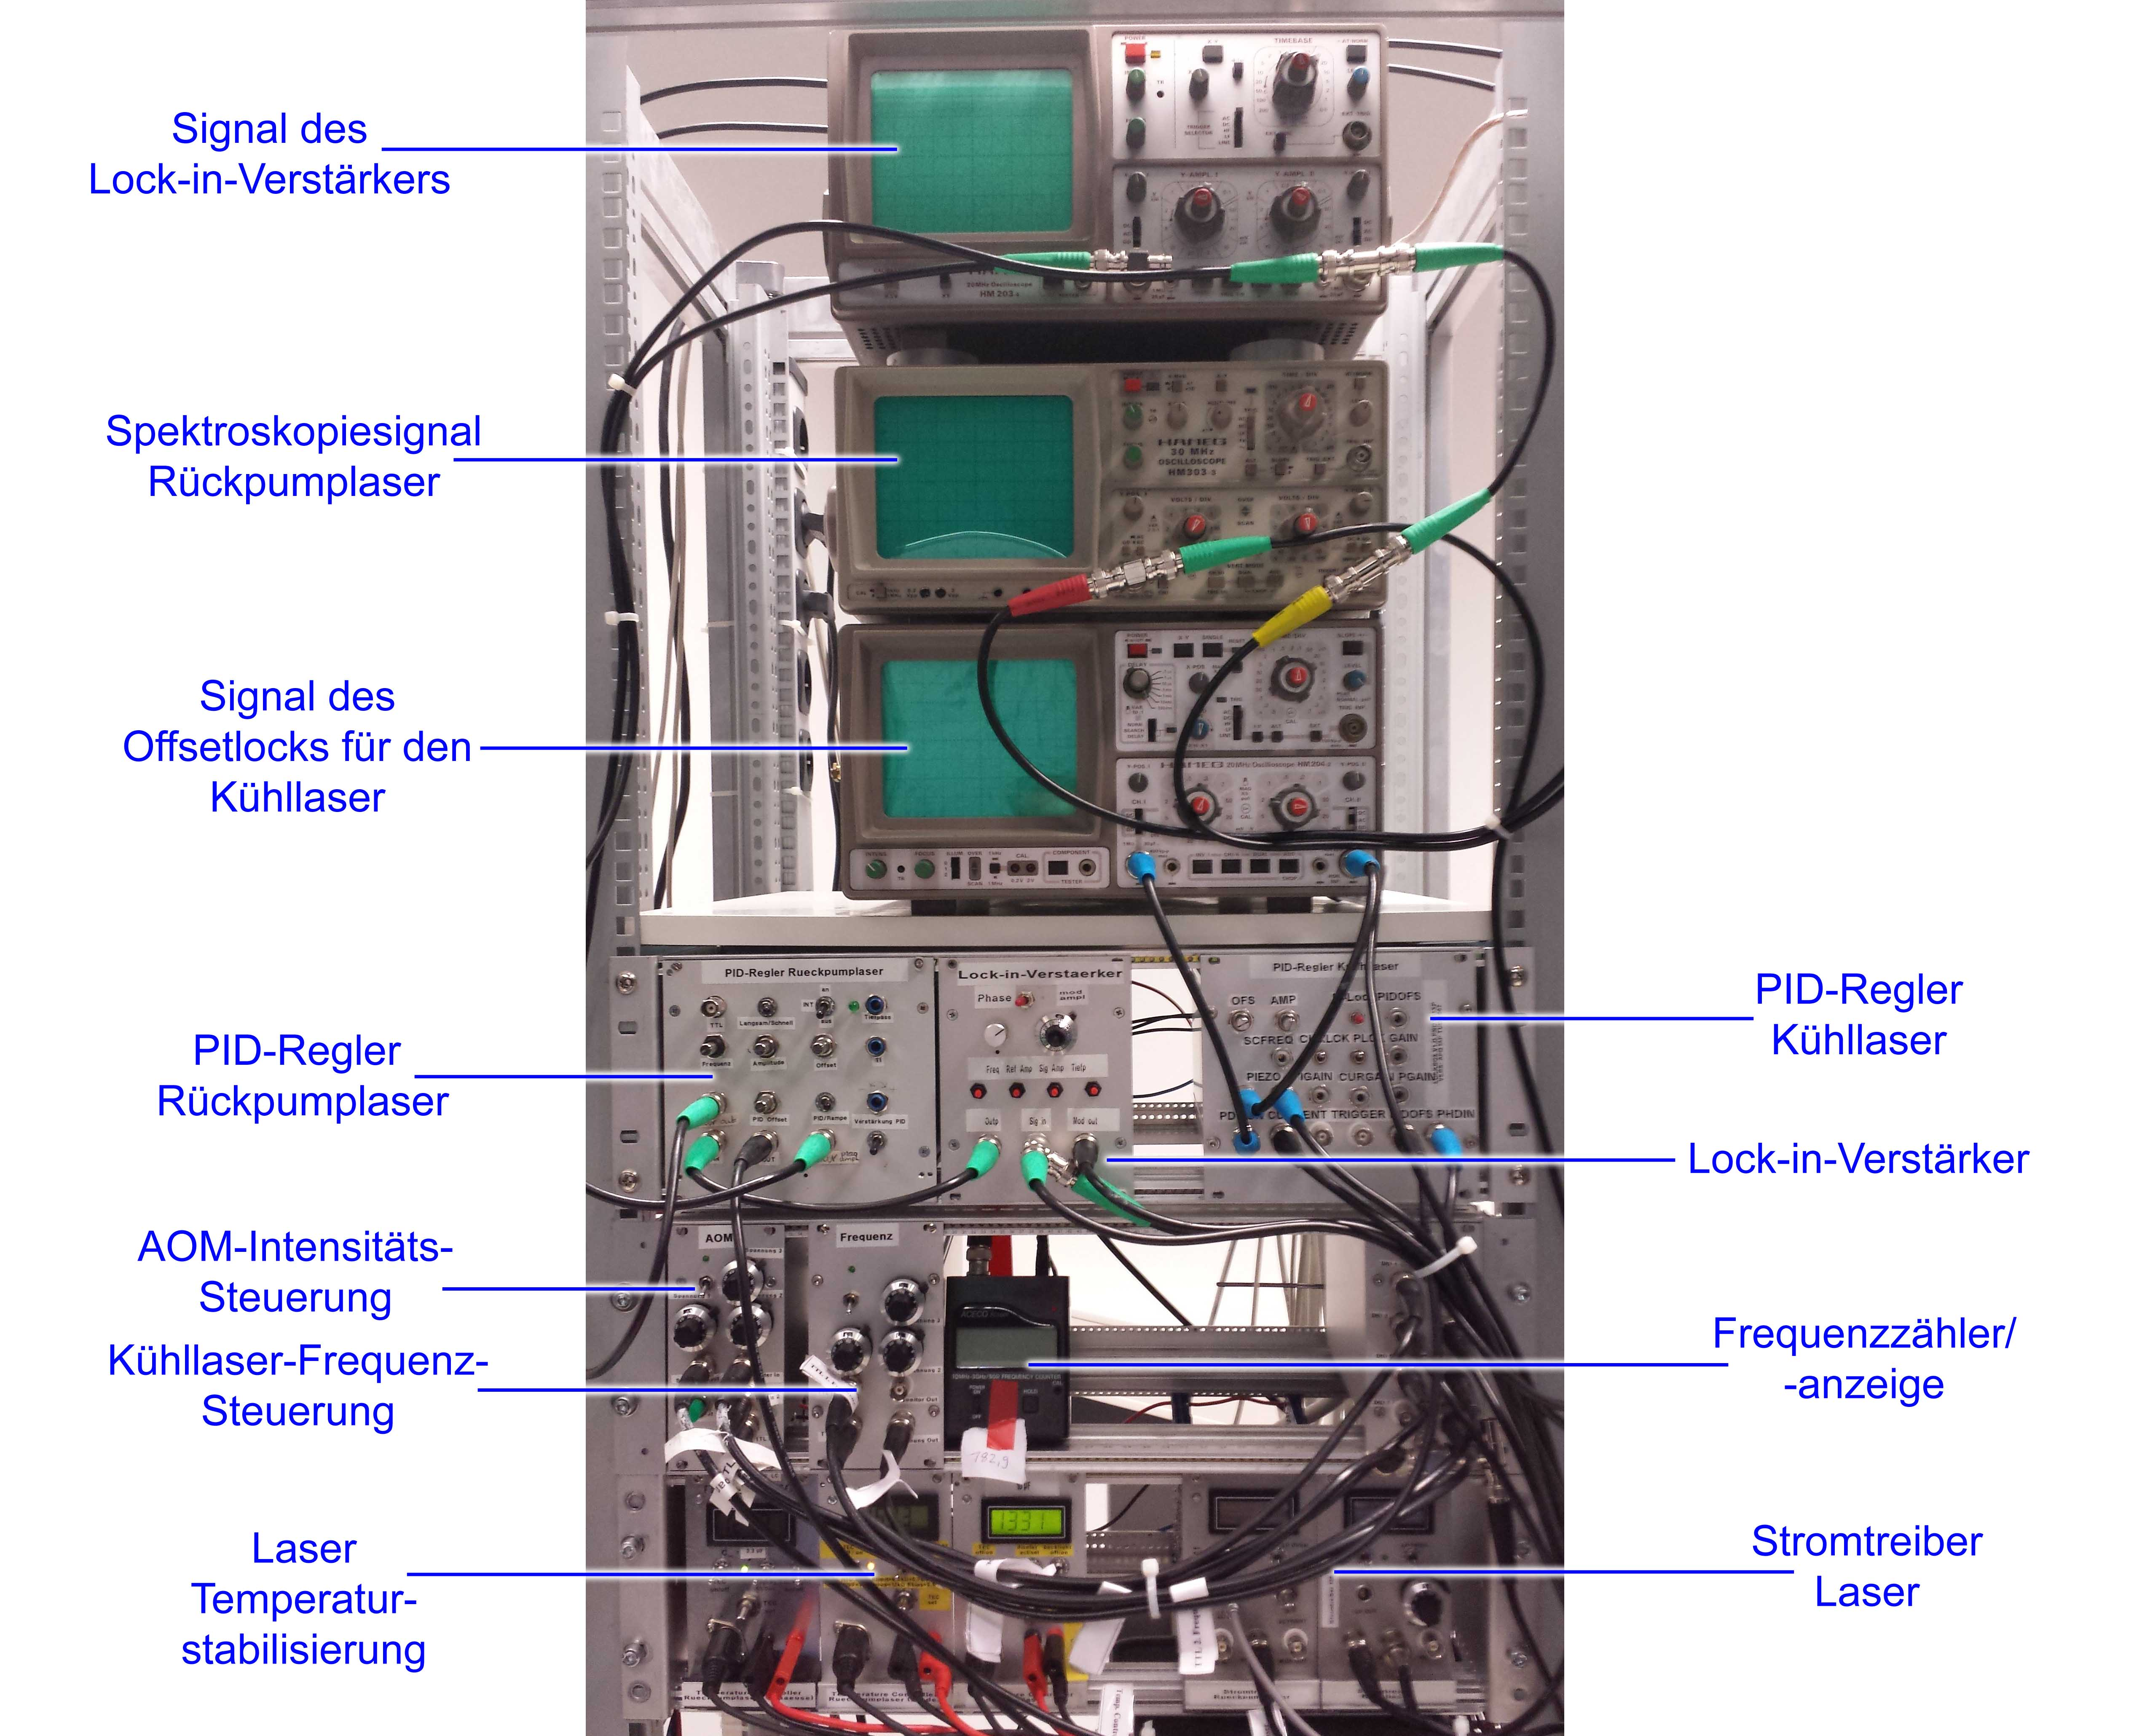
\includegraphics[width=480px]{Bilder/Rack2.jpg}
	\caption{Aufbau des Racks}
	\label{fig:Rack}
\end{figure} 

Um den Versuch zu verstehen und möglichst viel aus der Durchführung mitzunehmen sollten Sie sich schon während der Vorbereitung intensiv mit der Realisierung des Versuchsaufbaus vertraut machen. Dazu existiert im Anhang eine Bilderreihe, in welcher unterschiedliche Elemente des Aufbaus markiert sind. Diese können über die Links auf der nächsten Seite aufgerufen und sollten in die jeweiligen Betrachtungen mit einbezogen werden.\\
Eine detaillierte Beschreibung des Aufbaus sowie der Strahlführung findet sich in den entsprechenden Theoriekapiteln. Hier wird wiederum, wie zu Beginn erwähnt, Bezug auf dieses Kapitel genommen, um die Details in Bezug zum Gesamtaufbau zu betrachten.\\
Dieser ist mit allen markierten Elementen ebenfalls auf der nächsten Seite und im Anhang noch einmal dargestellt (siehe \autoref{fig:AEGBv}).\\


\fbox{\parbox[c]{17,2cm}{
		\begin{frage}\label{f:4-1}
			Welchen Vorteil bietet es, den Aufbau der MOT durch ein Glasfaserkabel von dem Aufbau der Laserstabilisierung zu trennen?
		\end{frage}
	}}\\

~\\

\centering



\begin{tabular}{lll}
	& \textbf{Markierte Elemente} & \textbf{Abbildung}\\
	& ~ & ~\\
	
\includegraphics[width=8px]{Bilder/Kaestchen/SL.jpg} & Spiegel der Laserstabilisierung u. ~ 
\includegraphics[width=8px]{Bilder/Kaestchen/SM.jpg} ~ der MOT& \autoref{fig:SL}\\
	
\includegraphics[width=8px]{Bilder/Kaestchen/ST.jpg} & Strahlteiler ~~ u. ~ 
\includegraphics[width=8px]{Bilder/Kaestchen/RD.jpg} ~ Rubidiumdampfzelle & \autoref{fig:SW}\\
	
\includegraphics[width=8px]{Bilder/Kaestchen/PD.jpg} & Photodioden \medspace u. ~ 
\includegraphics[width=8px]{Bilder/Kaestchen/UK.jpg} ~ USB-Kamera ~ & \autoref{fig:PD}\\
	
\includegraphics[width=8px]{Bilder/Kaestchen/LH.jpg} & $\lambda/2$-Platten ~ u. ~   
\includegraphics[width=8px]{Bilder/Kaestchen/LV.jpg} ~ $\lambda/4$-Platten & \autoref{fig:LH}\\
	
\includegraphics[width=8px]{Bilder/Kaestchen/LN.jpg} & Linsen & \autoref{fig:LI}\\
\end{tabular}

~\\
~\\
~\\

\begin{tabular}{lll}
	& \textbf{Markierte Strahlengänge} & \textbf{Abbildung}\\
	& ~ & ~\\
	
\includegraphics[width=8px]{Bilder/Kaestchen/RL.jpg} & Spektroskopie Rückpumplaser & \autoref{fig:SPM}\\
	
\includegraphics[width=8px]{Bilder/Kaestchen/SLS.jpg} & Spektroskopie Kühllaser & \autoref{fig:SPS}\\
	
\includegraphics[width=8px]{Bilder/Kaestchen/OL.jpg} & Offsetlock für den Kühllasers ~~~~~~~~~~~~~~~~~~~~~~~~~ & \autoref{fig:OFL}\\
	
\includegraphics[width=8px]{Bilder/Kaestchen/RL.jpg} & zur MOT Rückpumplaser & \autoref{fig:MM}\\
	
\includegraphics[width=8px]{Bilder/Kaestchen/SLS.jpg} & zur MOT Kühllaser & \autoref{fig:SZM}\\
	
\includegraphics[width=8px]{Bilder/Kaestchen/ML.jpg} & MOT & \autoref{fig:MOTSTG}\\
	
\includegraphics[width=8px]{Bilder/Kaestchen/AS.jpg} & alle Strahlengänge & \autoref{fig:STGK}\\
	& ~ & ~\\
	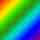
\includegraphics[width=8px]{Bilder/Kaestchen/AM.jpg} & alle Strahlengänge und alle Elemente  & \autoref{fig:AEGB}\\
	& (vgl. Abbildung 3) &
\end{tabular}

~\\
~\\
~\\

\begin{figure}[htb!]
	\centering
	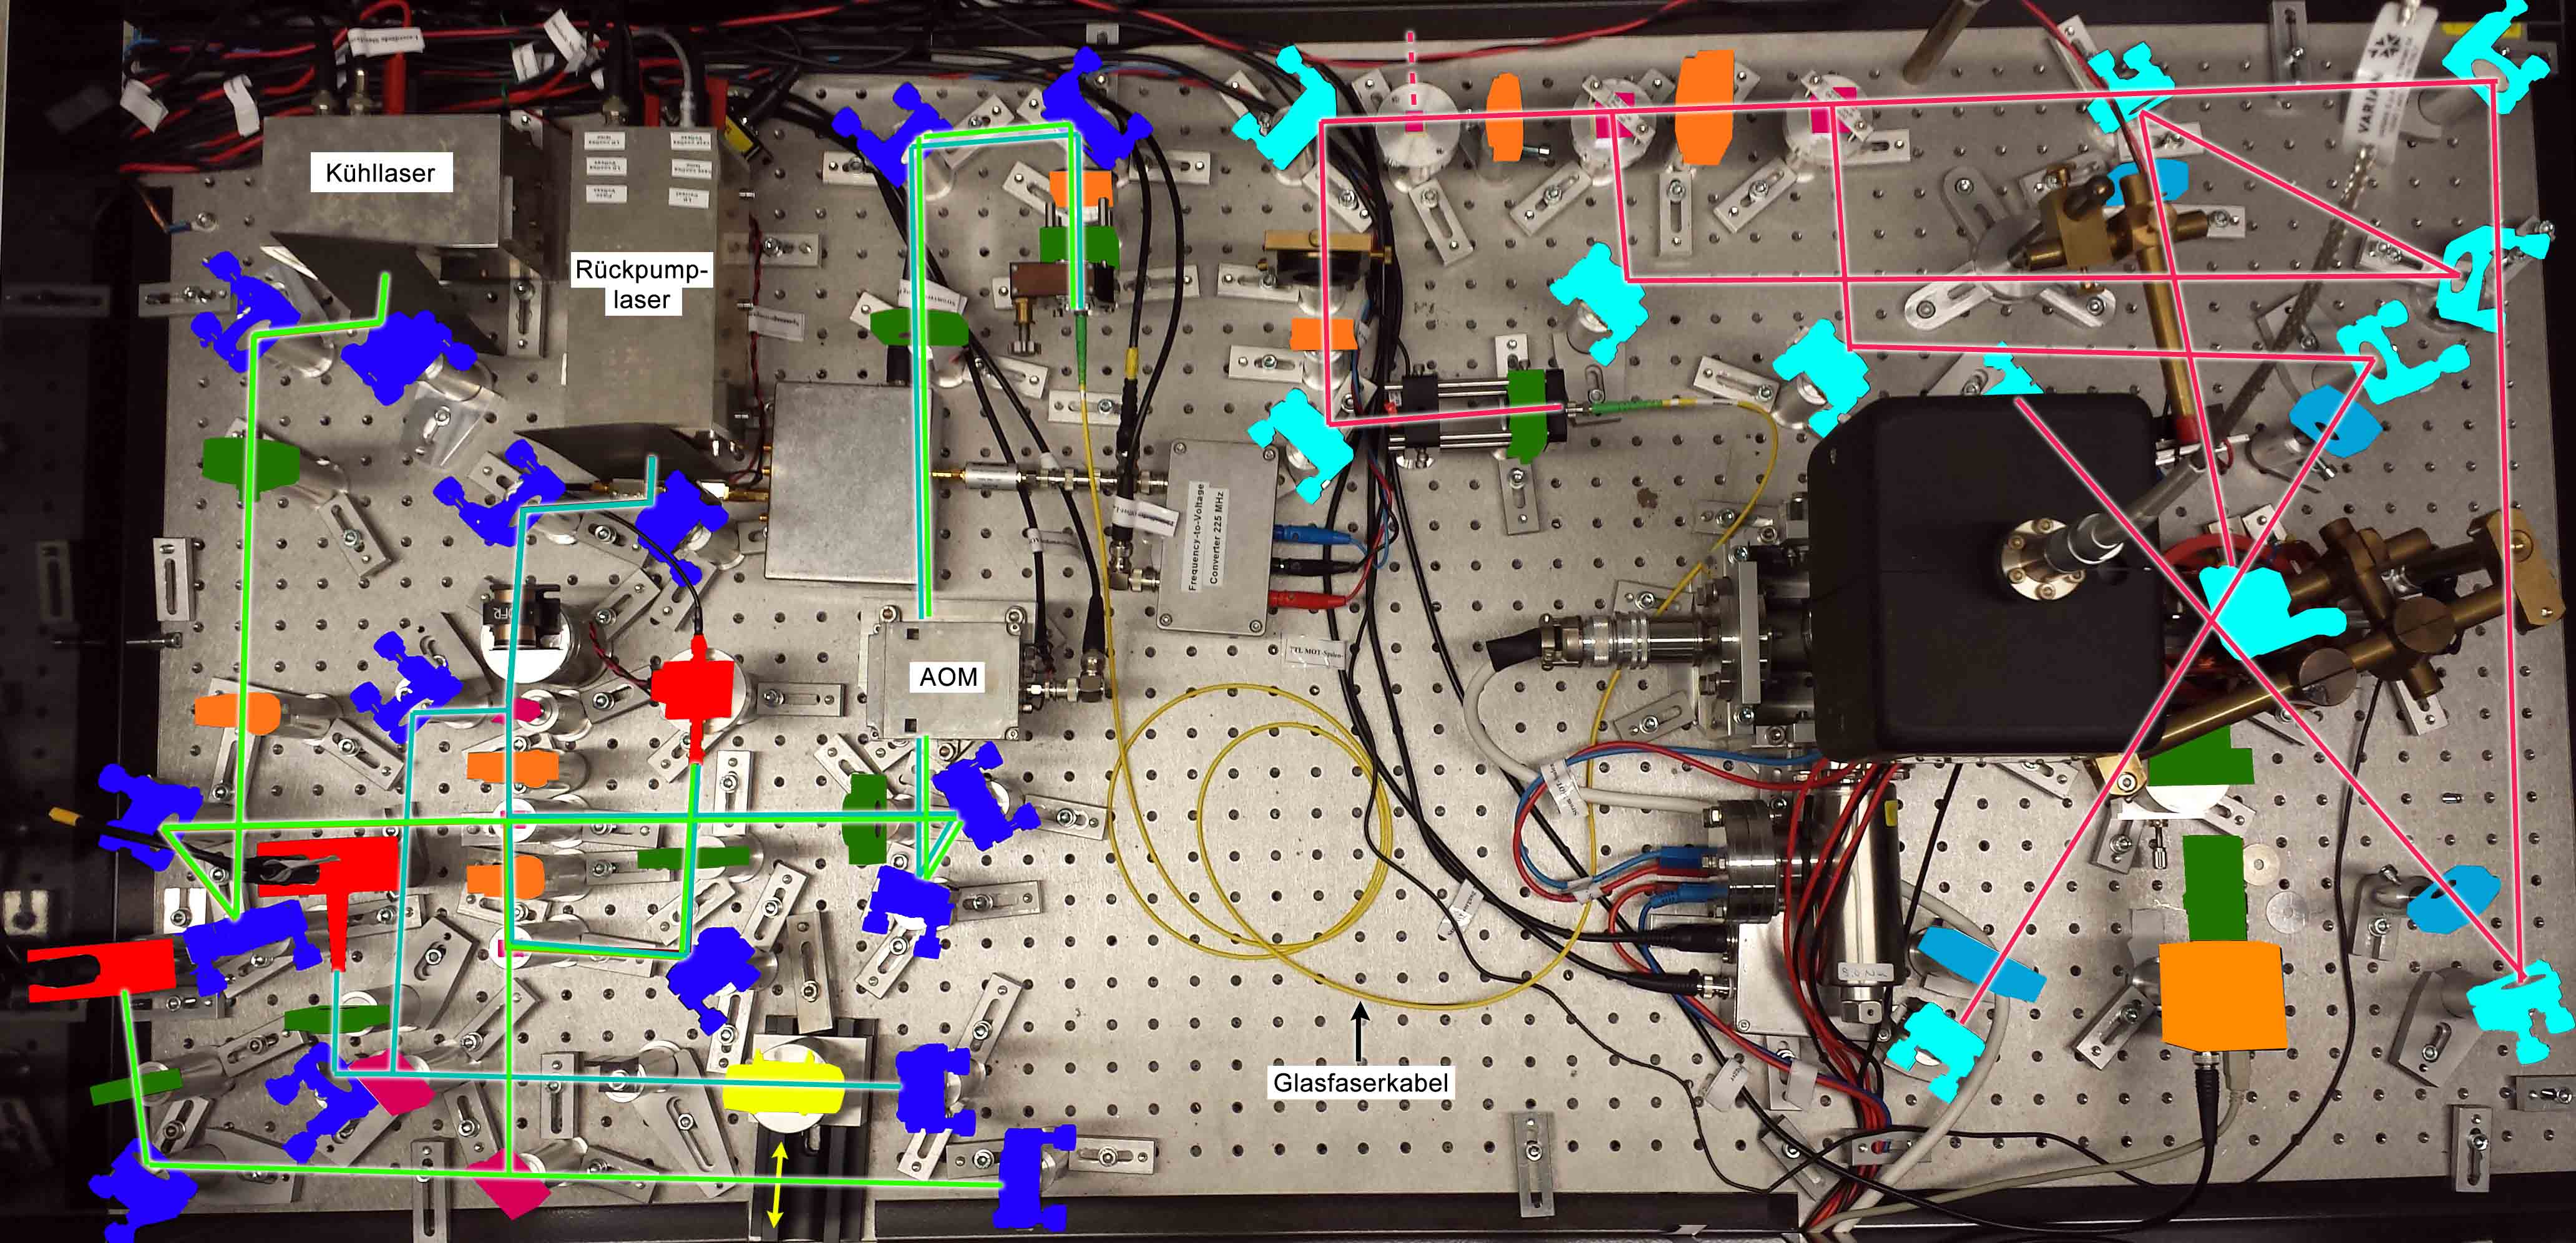
\includegraphics[width=480px]{Bilder/AEGB.jpg}
	\caption{Alle Strahlengänge und alle Elemente}
	\label{fig:AEGBv}
\end{figure}

Für die Variation der einzelnen Phasen des Versuchsablaufs in Dauer und Vorkommen wird ein LabVIEW-Programm verwendet. Dort kann der zyklische Durchlauf des Programms über die Benutzeroberfläche (siehe \autoref{fig:ES}) angepasst und kontrolliert werden.\\

\begin{figure}[htb!]
	\centering
	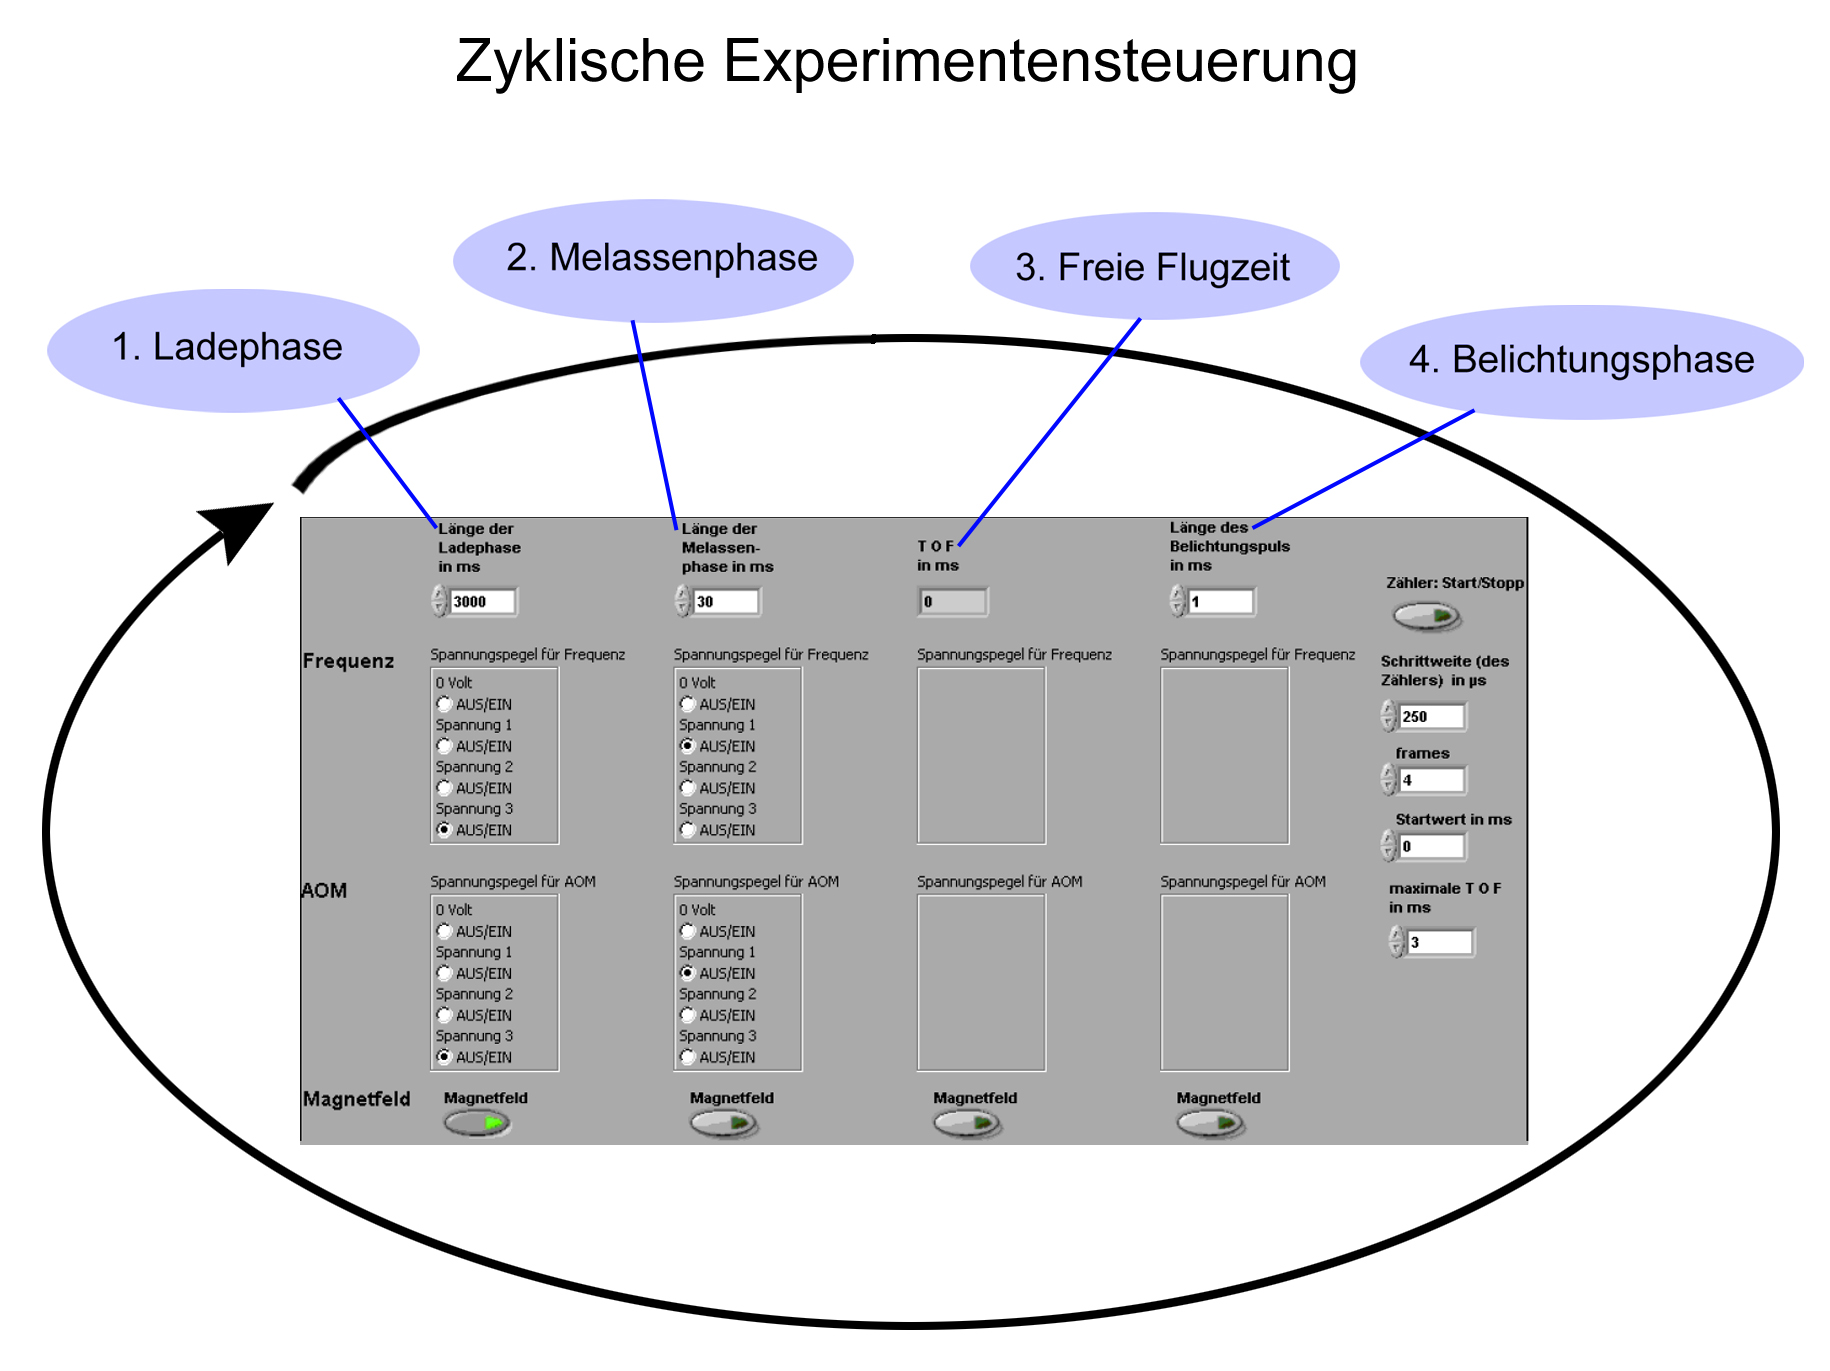
\includegraphics[width=480px]{Bilder/ES2.jpg}
	\caption{LabVIEW-Benutzeroberfläche zur Experimentensteuerung}
	\label{fig:ES}
\end{figure}

\newpage

\section{Wichtige Bauteile}

\subsection{Akusto-optischer Modulator (AOM)}

Ein akusto-optischer Modulator besteht im Wesentlichen aus einem Kristall, an dessen beiden Enden zum einen ein Piezoelement zur Erzeugung von Schallwellen und zum anderen ein Schallabsorber zum Verhindern von Reflexionen oder stehenden Wellen angebracht ist (siehe \autoref{fig:AOM}).\\
Die durch den Kristall propagierende Schallwelle, welche durch eine mechanische Schwingung des Piezoelements hervorgerufen wird, verursacht in diesem periodische Dichteschwankungen, welche eine ebenfalls periodische Variation der Brechzahl im Kristall zur Folge hat \cite{OLL}.\\
Diese Modulation wirkt für das einfallende Licht wie ein bewegtes optisches Gitter, an welchem Beugung des einfallenden Lichtes stattfindet. Dabei kommt es beim Betrieb im sogenannten Bragg-Regime lediglich zur Ausbildung der ersten Beugungsordnung. An dieser kann außerdem eine Frequenzverschiebung entsprechend der Schallfrequenz beobachtet werden. Um dies zu verstehen, kann dass Phänomen entweder klassisch oder im Teilchenbild betrachtet werden. Entsprechend der Betrachtungsweise kann der Effekt entweder mit Hilfe des Dopplereffekts durch das sich in Relation zum einfallenden Licht ``bewegende Gitter'' oder unter Anwendung der Impuls- und Energierhaltung auf die wechselwirkenden Photonen und Phononen beschrieben werden.\\
Bei Phononen handelt es sich in dieser Betrachtung um Quasiteilchen, mit welchen die den Kristall durchlaufenden Schallwellen beschrieben werden können \cite{OFI}.\\
Im Versuch wird der AOM im Wesentlichen als Schalter verwendet, um das Laserlicht zur MOT hin gezielt an- und abschalten zu können.\\

\fbox{\parbox[c]{17,2cm}{
		\begin{frage}\label{f:4-1}
			Inwiefern ist die durch den AOM verursachte Frequenzverschiebung des Laserlichts in Bezug auf die Stabilisierung des Rückpump- und Kühllasers bzw. die an der MOT benötigte Frequenz relevant?
		\end{frage}
	}}\\
	
	\begin{figure}[htb!]
		\centering
		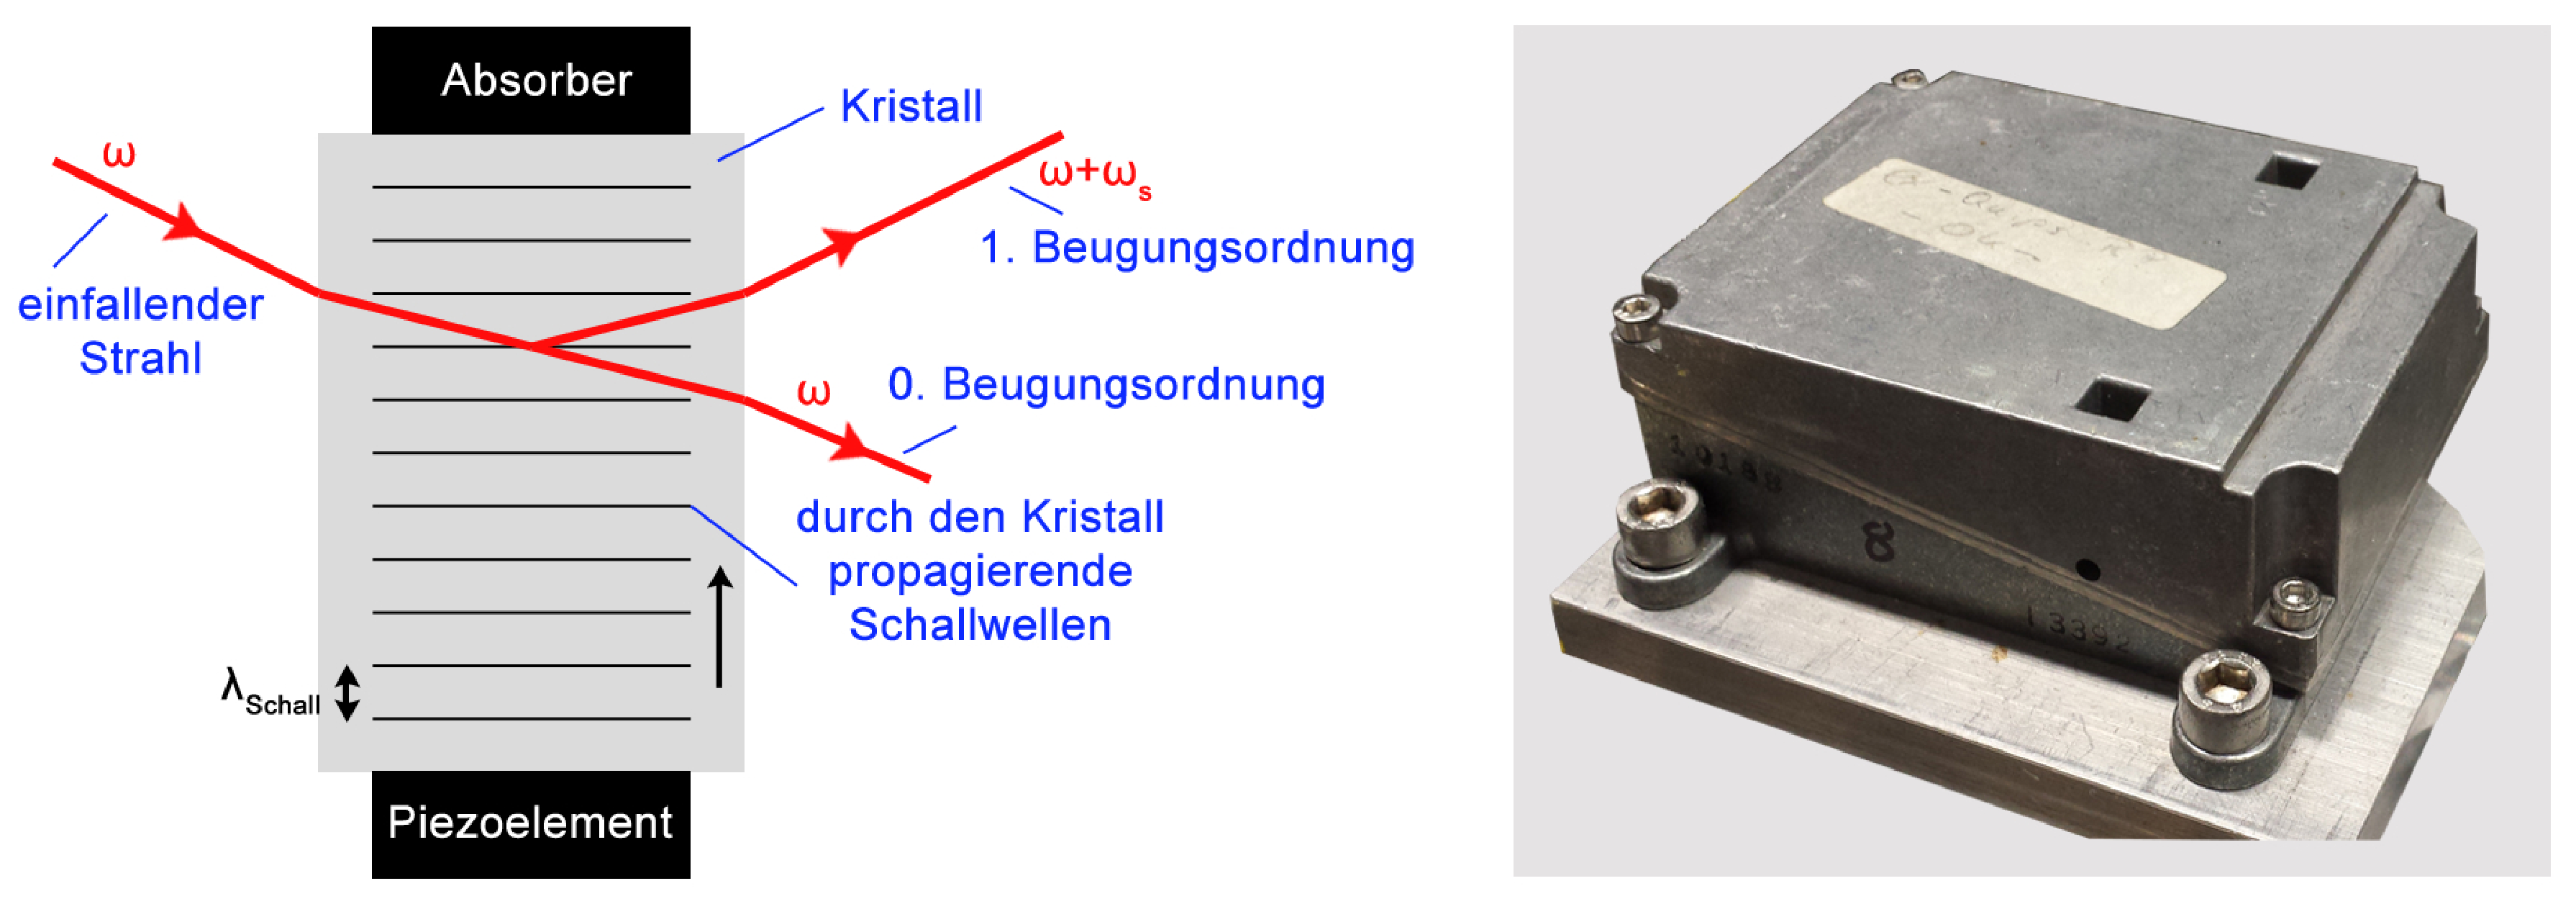
\includegraphics[width=480px]{Bilder/AOM2.pdf}
		\caption{Schematischer Aufbau eines AOMs mit skizziertem Strahlenverlauf des Laserlichts (links)
			und Darstellung des AOM-Gehäuses aus dem Versuchsaufbau (rechts)}
		\label{fig:AOM}
	\end{figure}
	
	\newpage
	
	\subsection{Verzögerungsplatten} \label{ssec:lambdaplatte}
	
Verzögerungsplättchen funktionieren nach dem Prinzip der Doppelbrechung und spielen sowohl bei der Erzeugung als auch bei der Analyse verschiedener Polarisationsformen des Lichtes eine zentrale Rolle.\\
Dabei liegt die optische Achse des Kristalls parallel zur Eintrittsfläche beziehungsweise senkrecht zur Ausbreitungsrichtung des einfallenden Lichts. Aus diesem Grund verlaufen sowohl der außerordentliche als auch der ordentliche Strahl, in welche der einfallende Lichtstrahl innerhalb des Materials durch Projektion auf die optische Achse zerlegt wird, parallel durch den Kristall.
Allerdings besitzen die beiden Strahlen dort unterschiedliche Ausbreitungsgeschwindigkeiten.\\
Aufgrund der Dicke des Kristalls und der damit verbundenen optischen Weglänge, welche beide Strahlen innerhalb des Kristalls zurücklegen, ergibt sich beim Austritt eine Phasendifferenz zwischen dem außerordentlichen und ordentlichen Anteil des Strahls. Dabei ist jedoch beispielsweise die einer Phasendifferenz von $\pi/2$ entsprechende Plättchendicke meist zu gering, um sie technisch realisieren zu können. Dies kann entweder dadurch behoben werden, dass auf die gewünschte Phasendifferenz ein Vielfaches von $2\pi$ addiert wird, um so eine größere Dicke zu erzielen oder man kombiniert zwei Plättchen mit gekreuzten optischen Achsen für den ordentlichen und außerordentlichen Strahl mit einer entsprechenden Gangdifferenz von $\pi$ oder $\pi/2$.\\
Falls nun linear polarisiertes Licht auf das Verzögerungsplättchen trifft, kann beispielsweise zirkular, elliptisch, oder wieder linear polarisiertes Licht mit veränderter Polarisation erzeugt werden \cite{OLL}.\\
Das Prinzip einer Verzögerungsplatte ist in \autoref{fig:LVPT} am Beispiel einer $\lambda/4$-Platte dargestellt.\\
	
\fbox{\parbox[c]{17,2cm}{
	\begin{frage}\label{f4-1}
				Zu welchem Zweck werden die in den schematischen Skizzen zur Laserstabilisierung und der MOT eingezeichneten Verzögerungsplatten jeweils verwendet? 
	\end{frage}
}}\\
		
	\begin{figure}[htb!]
			\centering
			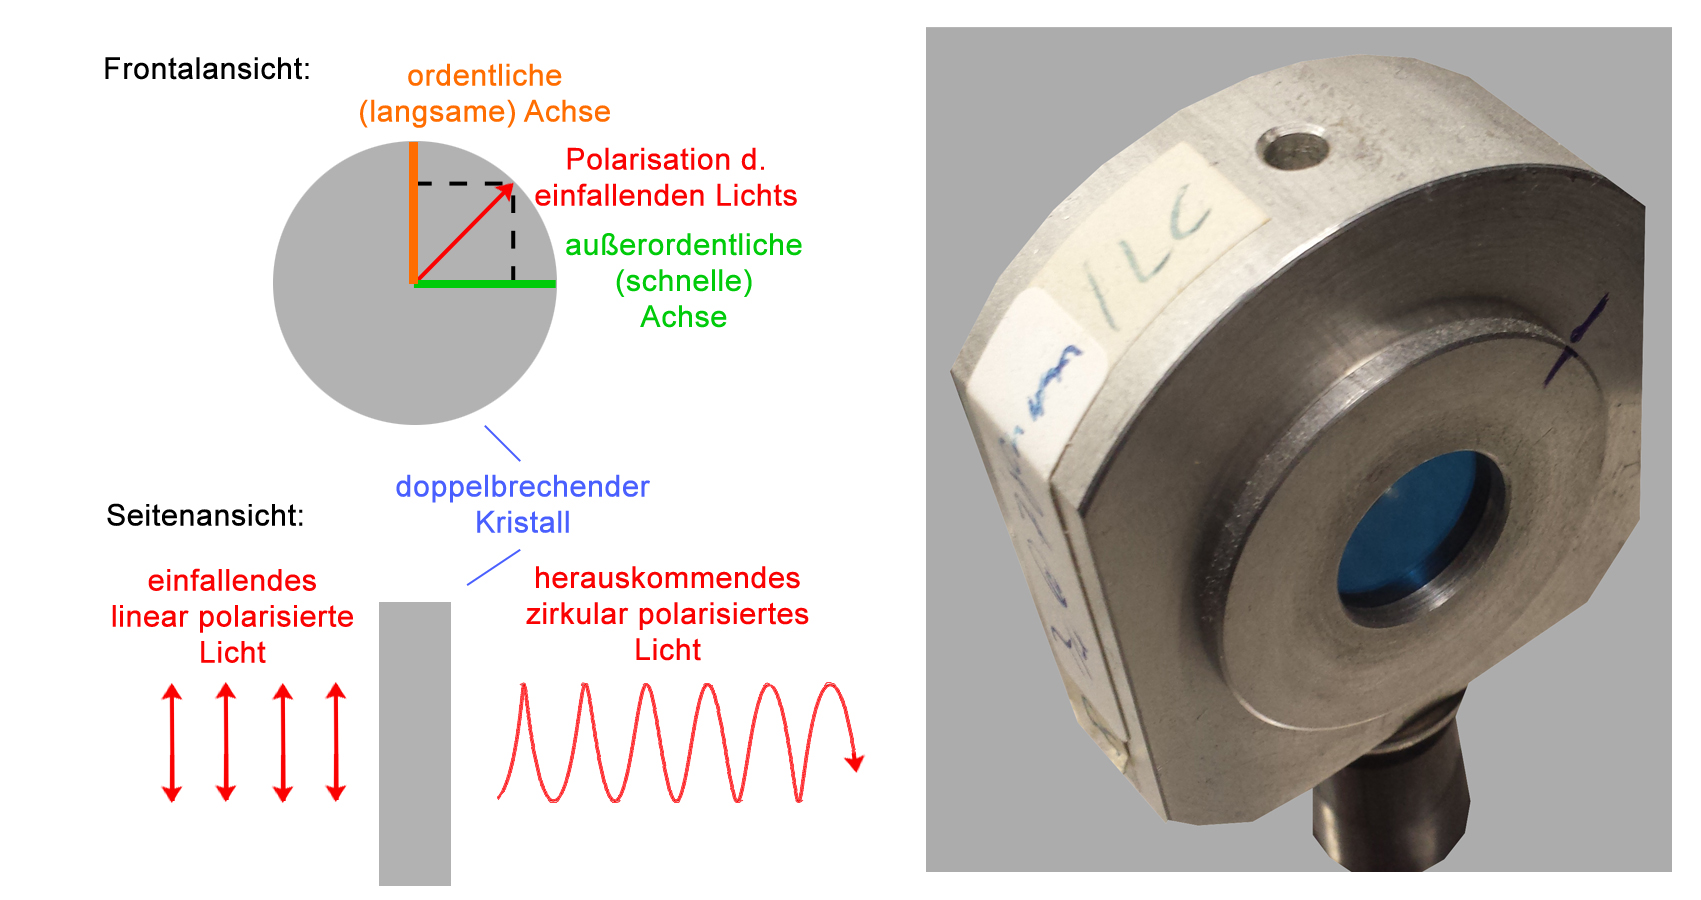
\includegraphics[width=480px]{Bilder/LVPT.jpg}
			\caption{Schematische Skizze zur Funktion einer $\lambda/4$-Platte (links)
				und Darstellung der im Versuch verwendeten $\lambda/4$-Platte (rechts)}
			\label{fig:LVPT}
		\end{figure}
		
		\newpage
		
		\subsection{Polarisationsstrahlteilerwürfel (PST)}
		
		Zur Realisierung von Strahlteilerwürfeln gibt es unterschiedliche Möglichkeiten. Eine dieser Möglichkeiten beruht auf dem zuvor diskutierten Prinzip der Doppelbrechung. Hier wird der unterschiedliche Brechungsindex für die beiden Polarisationsrichtungen verwendet, um die Bedingungen für Totalreflexion für eine dieser Komponenten zu erfüllen.\\
		Es gibt allerdings auch andere Möglichkeiten Strahlteilerwürfel herzustellen. Diese zweite Realisierungsmöglichkeit entspricht dem Aufbau der im Versuch verwendeten Strahlteilerwürfel (siehe \autoref{fig:PST}).\\ 
		Statt doppelbrechenden Kristallen werden hier Dünnschichtpolarisatoren verwendet. Der zugehörige Aufbau besteht aus einem Würfel aus isotropem Glas, welcher diagonal aufgeschnitten wird. Zwischen die beiden entstandenen Prismen wird ein Dünnschichtpolarisator eingebracht, bevor alles wieder miteinander verkittet wird. Dieser besteht, ähnlich einem Bragg-Spiegel, aus vielen dünnen dielektrischen Schichten, welche ein unterschiedliches Reflexionsvermögen für die beiden betrachteten Polarisationsrichtungen besitzen (siehe \autoref{fig:PST}). Wählt man die Schichtdicke so, dass sich die an den einzelnen Schichten reflektierten (s-polarisierten) Anteile konstruktiv überlagern, hat man die Bedingungen für eine erfolgreiche Polarisationstrennung erfüllt \cite{EX}.\\
		
		\fbox{\parbox[c]{17,2cm}{
				\begin{frage}\label{f4-1}
					Zu welchem Zweck werden die PST verwendet und warum kommen sie stets in Kombination mit einer $\lambda/2$-Platte vor?  
				\end{frage}
			}}\\
			
			\begin{figure}[htb!]
				\centering
				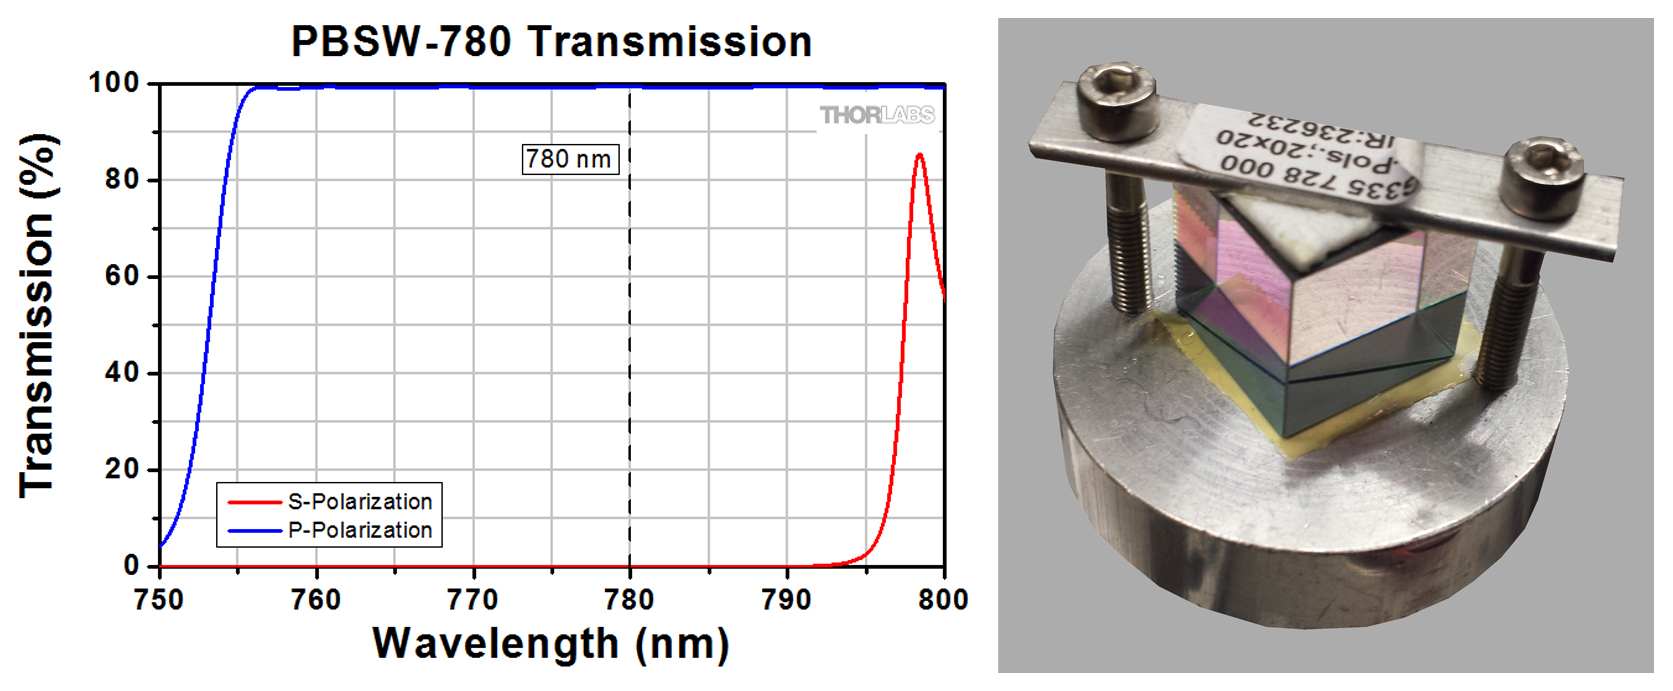
\includegraphics[width=480px]{Bilder/DP.jpg}
				\caption{Reflektivität in Abhängigkeit von der Wellenlänge füt s- und p-Polarisation (links) \cite{POL}
				und Darstellung eines im Versuch verwendeten Strahlteilerwürfels (rechts)}
				\label{fig:PST}
			\end{figure}
			
			\newpage
			
			\subsection{Photodiode}
			
			In diesem Kapitel soll kurz auf den Aufbau und das Funktionsprinzip einer Photodiode eingegangen werden, da diese sowohl zur Aufnahme des Spektroskopiesignals des Rückpump- und Kühllasers als auch zur Aufnahme des Schwebungssignals für den \nameref{ssec:Offsetlock} zur Stabilisierung des Kühllasers verwendet wird.\\
			Dies soll am Beispiel einer pin-Photodiode erfolgen. Diese besteht aus einem n-dotierten Halbleiter, der un- oder sehr schwach dotierten i-Schicht, welche zur Vergrößerung der Raumladungszone führt und einem p-dotierten Halbleiter (siehe \autoref{fig:PDI}). Durch Rekombination der Elektronen des n-dotierten Halbleiters mit den Löchern des p-dotierten Halbleiters kommt es zur Ausbildung einer Raumladungszone, bis die entstehende Diffusionsspannung ein weiteres Eindringen der jeweiligen Ladungsträger in das andere Gebiet verhindert. Wird nun die Diode mit Licht bestrahlt, kommt es bei der Absorption von Photonen zur Ausbildung von Elektron-Loch-Paaren, welche im elektrischen Feld der Raumladungszone (in der i-Schicht) voneinander getrennt werden. Diese Ladungsträger fließen als messbarer Photostrom über die Kontakte ab.\\
			Die p-Schicht der Diode ist hier vergleichsweise dünn ausgeführt, damit in dieser möglichst wenig Licht absorbiert wird und dieses ungehindert in die i-Schicht gelangen kann, um die dort benötigten Elektron-Loch-Paare zu erzeugen.\\
			
			\begin{figure}[htb!]
				\centering
				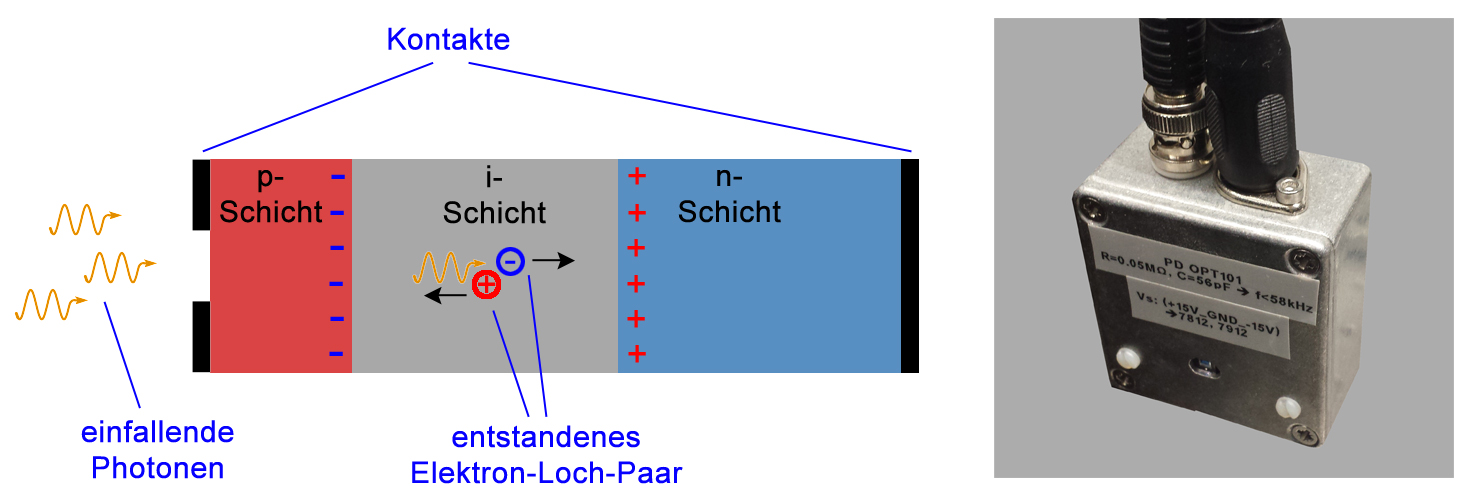
\includegraphics[width=480px]{Bilder/PDI.jpg}
				\caption{Aufbau einer pin-Photodiode (links)
					und Darstellung einer im Versuch verbauten Version (rechts)}
				\label{fig:PDI}
			\end{figure}
			
			
			
			\subsection{Ionen-Getter-Pumpe}
			
			Eine wichtige Rolle für den Versuch spielt die sogenannte Ionen-Getter-Pumpe, da diese einerseits zur Erzeugung und andererseits zur Aufrechterhaltung des für die Realisierung der MOT benötigten Vakuums verwendet wird.\\
			Aus diesem Grund ist die Pumpe auch ständig in Betrieb, um die Leckrate des Systems zu kompensieren. Der etwas komplexere Aufbau der Ionen-Getter-Pumpe lässt sich in mehrere benötigte Komponenten zerlegen. Der Hauptteil der Pumpe besteht aus vielen aneinandergeschweißten Metallröhrchen, welche sich zwischen zwei äußeren Blechen befinden (siehe \autoref{fig:IGP}). Zwischen den Röhrchen und den Blechen existiert ein kleiner Spalt, welcher einerseits dem Gas erlaubt in die Röhrchen einzuströmen und andererseits zur elektrischen Isolation (in Kombination mit Keramikisolatoren) zwischen Röhrchen und Blechen dient. Nun wird zwischen den Blechen (Kathoden) und den Röhrchen (Anode) eine Hochspannung angelegt, wobei die Bleche auf gleichem Potential sind. Dadurch wird eine Elektronenwolke erzeugt. Durch zwei von außen angebrachte Permanentmagnete und das daraus resultierende Magnetfeld werden die freien Elektronen auf eine Spiralbahn gezwungen.\\
			
			\newpage
			
			Treffen diese nun auf Atome des eingeströmten Gases (hier Rubidium) kommt es zu einer Stoßionisation dieser Atome. Die zurückbleibenden positiven Ionen werden durch das elektrische Feld in Richtung Kathode beschleunigt. Auf ihrem Weg zur Kathode besteht die Möglichkeit, dass sie durch Stöße mit neutralen Atomen weitere Ionen erzeugen. Im Idealfall treffen die Ionen schließlich mit hoher kinetischer Energie auf das Kathodenmaterial, dass sie durch den Aufprall ``aufwirbeln'' und so dafür sorgen, dass stets frisches Material an der Oberfläche zur Verfügung steht. Letztendlich gehen sie nach dem Aufprall eine chemische Bindung mit dem Kathodenmaterial ein und stehen dadurch nicht mehr im gasförmigen Zustand bereit \cite{IGP}.\\ 
			
			\textbf{ACHTUNG:} Für die Vorbereitung muss nur das grundlegende Prinzip der Pumpe verstanden sein. Die detaillierten Ausführungen bezüglich der technischen Details sind für besonders Interessierte gedacht.\\
			
			\begin{figure}[htb!]
				\centering
				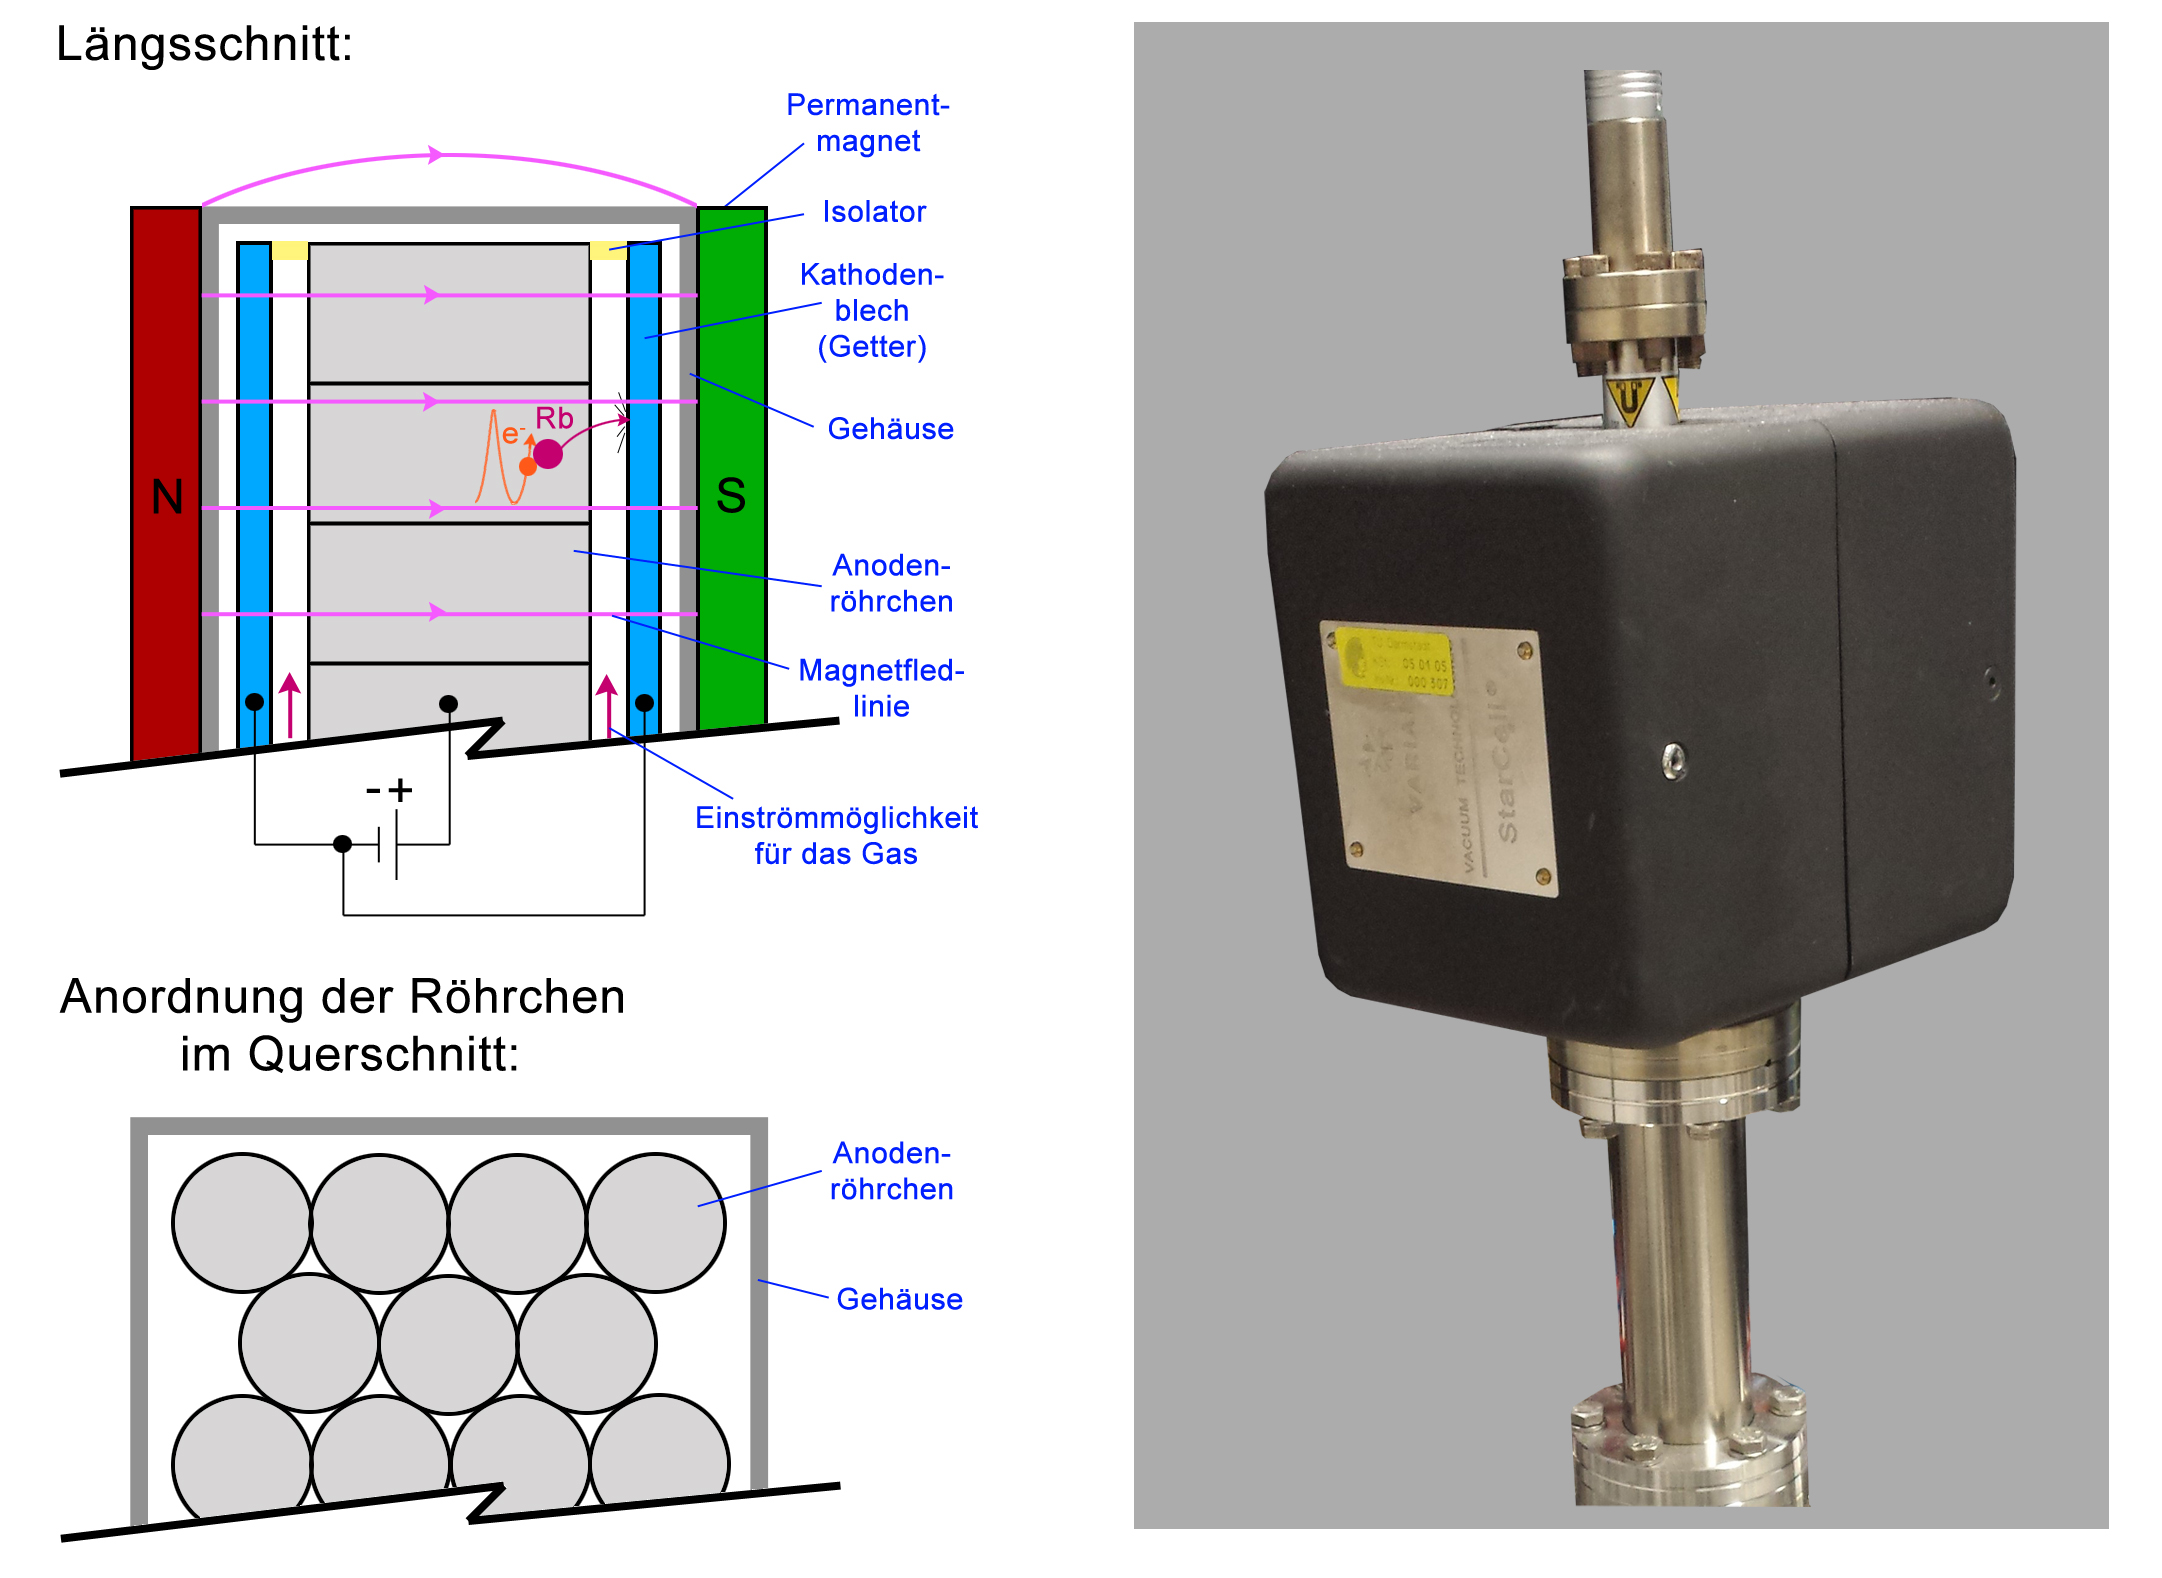
\includegraphics[width=480px]{Bilder/IGP.jpg}
				\caption{Schematische Skizze des Aufbaus einer Ionen-Getter-Pumpe (links) und Darstellung der im Versuch verwendeten Ionen-Getter-Pumpe (rechts)}
				\label{fig:IGP}
			\end{figure}
			
			\newpage
			
			\subsection{PID-Regler}
			
			Der PID-Regler ist ein Element, welches zur Stabilisierung der Laser verwendet wird. Dabei setzt sich dieser aus drei einzelnen Regeleinrichtungen (der proportionalen, der integrierenden und der differenzierenden Regeleinrichtung) zusammen.\\
			Erst das Zusammenspiel dieser drei einzelnen Regeleinrichtungen in Hinblick auf ihr jeweiliges charakteristisches Verhalten führt zu den gewünschten positiven Eigenschaften des PID-Reglers. Darum sollen zunächst die einzelnen Komponenten mit ihren Charakteristika kurz andiskutiert werden.\\
			Hierzu muss jedoch zuerst der Aufbau eines Regelkreises beziehungsweise dessen Funktionsweise verstanden werden. Ziel des Regelkreises ist es eine physikalische Größe \textit{x} (die Regelgröße) unabhängig von wirkenden Störgrößen \textit{z} auf einen gewählten Sollwert $x_S$ zu stabilisieren. Um dies zu gewährleisten wird der Istwert der Regelgröße $x_i$ (also der momentane tatsächliche Wert) mit dem Sollwert verglichen. Die Abweichung dieser beiden Größen voneinander (die Regelabweichung $x_W$) bestimmt letztlich die Ausgabe der sogenannten Regelgröße \textit{y}, durch deren Einfluss auf die Regelstrecke mögliche Abweichungen vom Sollwert ausgeglichen werden sollen.\\ 
			Der Proportionalregler (kurz P-Regler) ist der einfachste bekannte stetige Regler. Er gibt eine Ausgangsgröße \textit{y} (Regelgröße) aus, welche proportional zur Eingangsgröße $x_W$ (Regelabweichung) ist. Die Vorteile dieses Reglers liegen in seiner schnellen Stellgeschwindigkeit. Der entscheidende Nachteil des Reglers liegt jedoch darin, dass er eine bleibende Regelabweichung mit sich bringt. Das heißt, dass eine Regelabweichung nur eingeschränkt, jedoch nicht vollständig beseitigt werden kann.\\
			Dafür ist der Integralregler (kurz I-Regler) zuständig. Er gibt eine Stellgröße \textit{y} aus, welche proportional dem zeitlichen Integral über die Regelabweichung $x_W$ ist. Dadurch ist er in der Lage, auch kleine durch den P-Regler nicht beseitigte Abweichungen zu eliminieren, wenn auch vergleichsweise langsam.
			Um nun die Reaktionsgeschwindigkeit, speziell bei schnell entstehenden großen Abweichungen zu verbessern, wird noch der Differentialanteil (D-Anteil) benötigt. Er zeichnet sich dadurch aus, dass er eine Regelgröße \textit{y} ausgibt, die durch die Änderungsgeschwindigkeit der Regelgröße bestimmt wird. Er reagiert also auf den Differentialquotienten der Regelabweichung $x_W$. Der Einsatz dieses Reglers ist jedoch nur in Kombination mit den anderen Anteilen sinnvoll, da er auf eine zeitlich konstante (auch sehr große) Abweichung gar nicht reagiert. In Summe (siehe \autoref{fig:PID}) ergibt sich nun aber ein guter schneller Regler - der PID-Regler \cite{PID}.\\ 
			
			\begin{figure}[htb!]
				\centering
				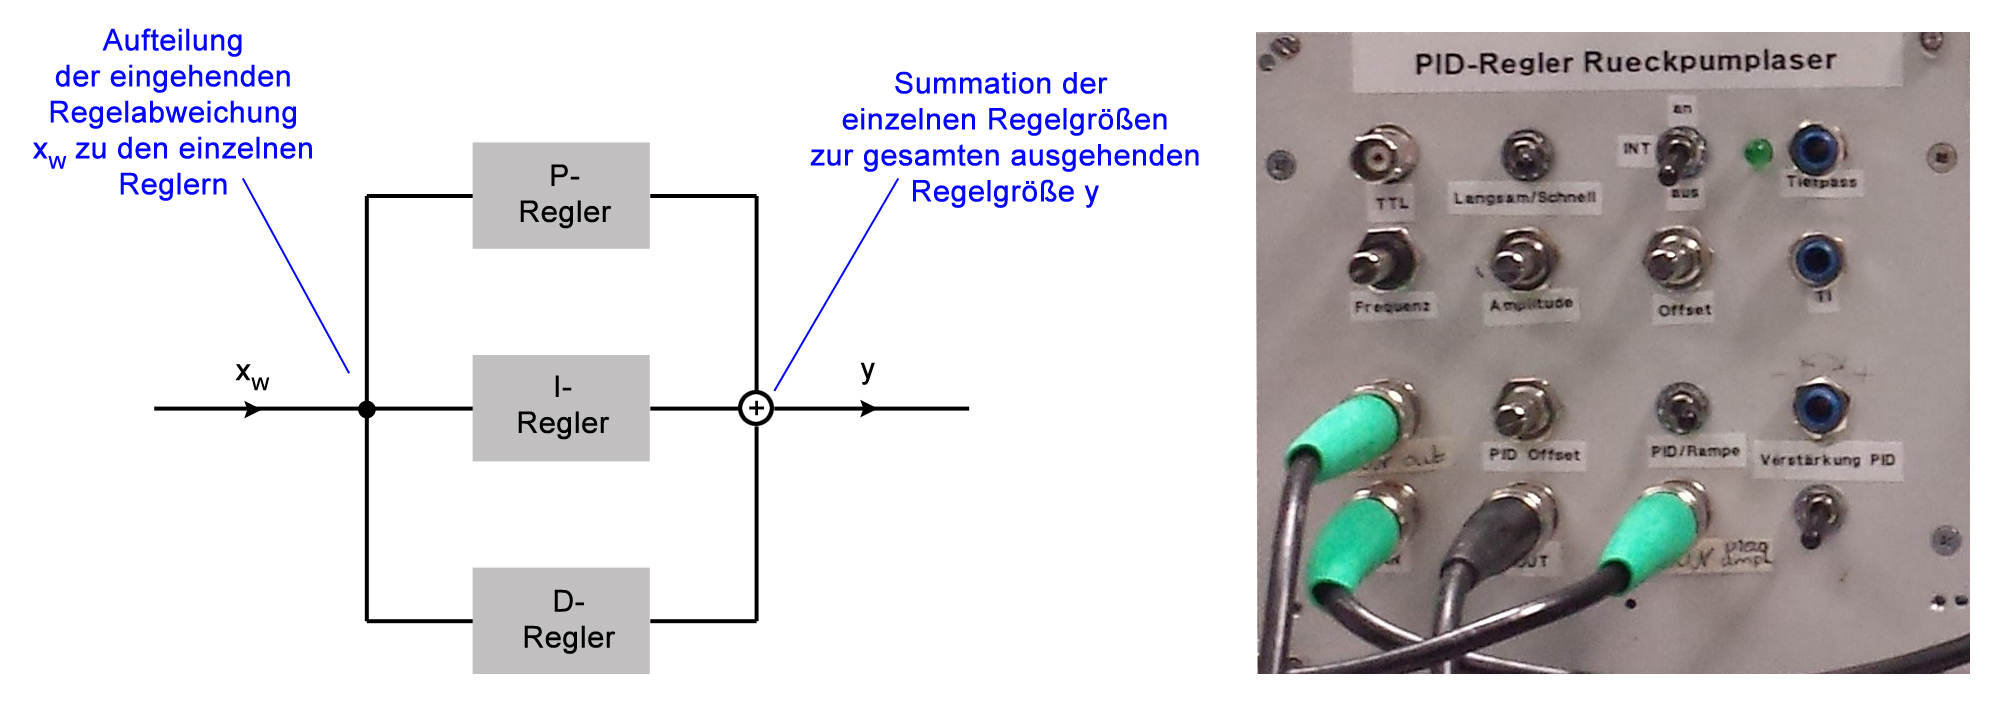
\includegraphics[width=480px]{Bilder/PID.jpg}
				\caption{Schematische Skizze des Funktionsweise bzw. Zusammensetzung eines PID-Reglers (links)
					und Darstellung der im Versuch verbauten Version (rechts)}
				\label{fig:PID}
			\end{figure}
			
			\newpage
			
			\section{Theorie zur Laserstabilisierung}
			
			\subsection{Aufbau der Laserstabilisierung}
			
			Das Lasersystem befindet sich auf der einen Hälfte einer optischen Tischplatte und wurde auf eine Strahlhöhe von 100mm einjustiert. Im Wesentlichen besteht es aus den zwei Lasern und deren Stabilisierungen. Ein Laser wird durch eine dopplerfreie Sättigungspektroskopie auf die Frequenz des Rückpumpübergangs stabilisiert. Er soll im Folgenden als Rückpumplaser bezeichnet werden. Der zweite Laser soll auf die Frequenz des Kühlübergangs gelockt werden. Diese Stabilisierung erfolgt durch einen Offsetlock relativ zur Frequenz des Rückpumplasers. Er soll im Folgenden Kühllaser genannt werden.\\
			In \autoref{fig:TZ} ist der Aufbau des Systems schematisch dargestellt. Das Licht des Rückpumplasers durchläuft zuerst einen Faraday-Isolator, um Rückreflexe in den Laser zu unterdrücken. Anschließend werden aus dem Strahl des Rückpumplasers 4\% für die Spektroskopie ausgekoppelt. Der transmittierte Teil des Lichts trifft nach Durchlaufen einer $\lambda/2$-Verzögerungsplatte auf einen polarisierenden Strahlteiler. In dem Strahlteiler wird der Strahl des Rückpumplasers mit dem des Kühllasers überlagert. Ein ausgehender Strahl bestehend aus Kühl- und Rückpumplicht wird durch einen akusto-optischen Modulator (AOM) gestrahlt, um dann in eine Glasfaser eingekoppelt zu werden, in der das Licht zur MOT geleitet wird.\\
			Der zweite ausgehende Strahl durchläuft wiederum eine $\lambda/2$-Verzögerungsplatte und trifft auf einen zweiten, polarisierenden Strahlteiler. Der s-polarisierte Anteil wird abgelenkt und mittels einer Linse auf eine schnelle Photodiode fokussiert. Das überlagerte Licht kann dort zur Stabilisierung des Kühllasers mittels eines Offsetlocks verwendet werden.\\
			Das Licht, das durch den Strahlteiler transmittiert, kann, indem die Rubidiumdampfzelle verschoben wird, ebenfalls für eine dopplerfreie Sättigungsspektroskopie des Kühllasers eingesetzt werden.\\
			
			\subsection{Verwendete Lasertypen}
			
			Zur Erzeugung des Lichts werden zwei Diodenlaser verwendet, deren Emissionswellenlänge mit Hilfe von Stromänderungen und Änderungen am externen Resonator beeinflusst werden kann.\\
			Ein Diodenlaser ist in der so genannten Littrow-Anordnung aufgebaut (siehe \autoref{fig:LLA}).\\ 
			Das Licht aus dem Halbleiter trifft so auf ein optisches Gitter, dass die minus erste Beugungsordnung in die Diode zurückreflektiert wird. Durch diese Anordnung bildet das Gitter zusammen mit der Rückseite der Diode den externen Resonator. Die nullte Beugungsordnung des Gitters wird aus dem Resonator ausgekoppelt. Zur groben Einstellung der Frequenz kann das Gitter gedreht, durch Längenänderung des Resonators kann die Frequenz fein eingestellt werden.\\
			Der zweite Diodenlaser besitzt als frequenzselektives Element einen Interferenzfilter. Auch dieser Laser kann durch Längenänderung des externen Resonator (hier: ein Auskoppelspiegel auf einem Piezokristall) und dem Strom durch die Laserdiode in der emittierten Frequenz durchgestimmt werden.\\
			
			\fbox{\parbox[c]{17,2cm}{
					\begin{frage}
						Durch welche Größen/Faktoren werden die Laserfrequenzen beeinflusst? Welche dieser Faktoren sind gewollt beziehungsweise ungewollt und wie können diese beseitigt werden?
					\end{frage}
				}}\\
				
				\begin{figure}[htb!]
					\centering
					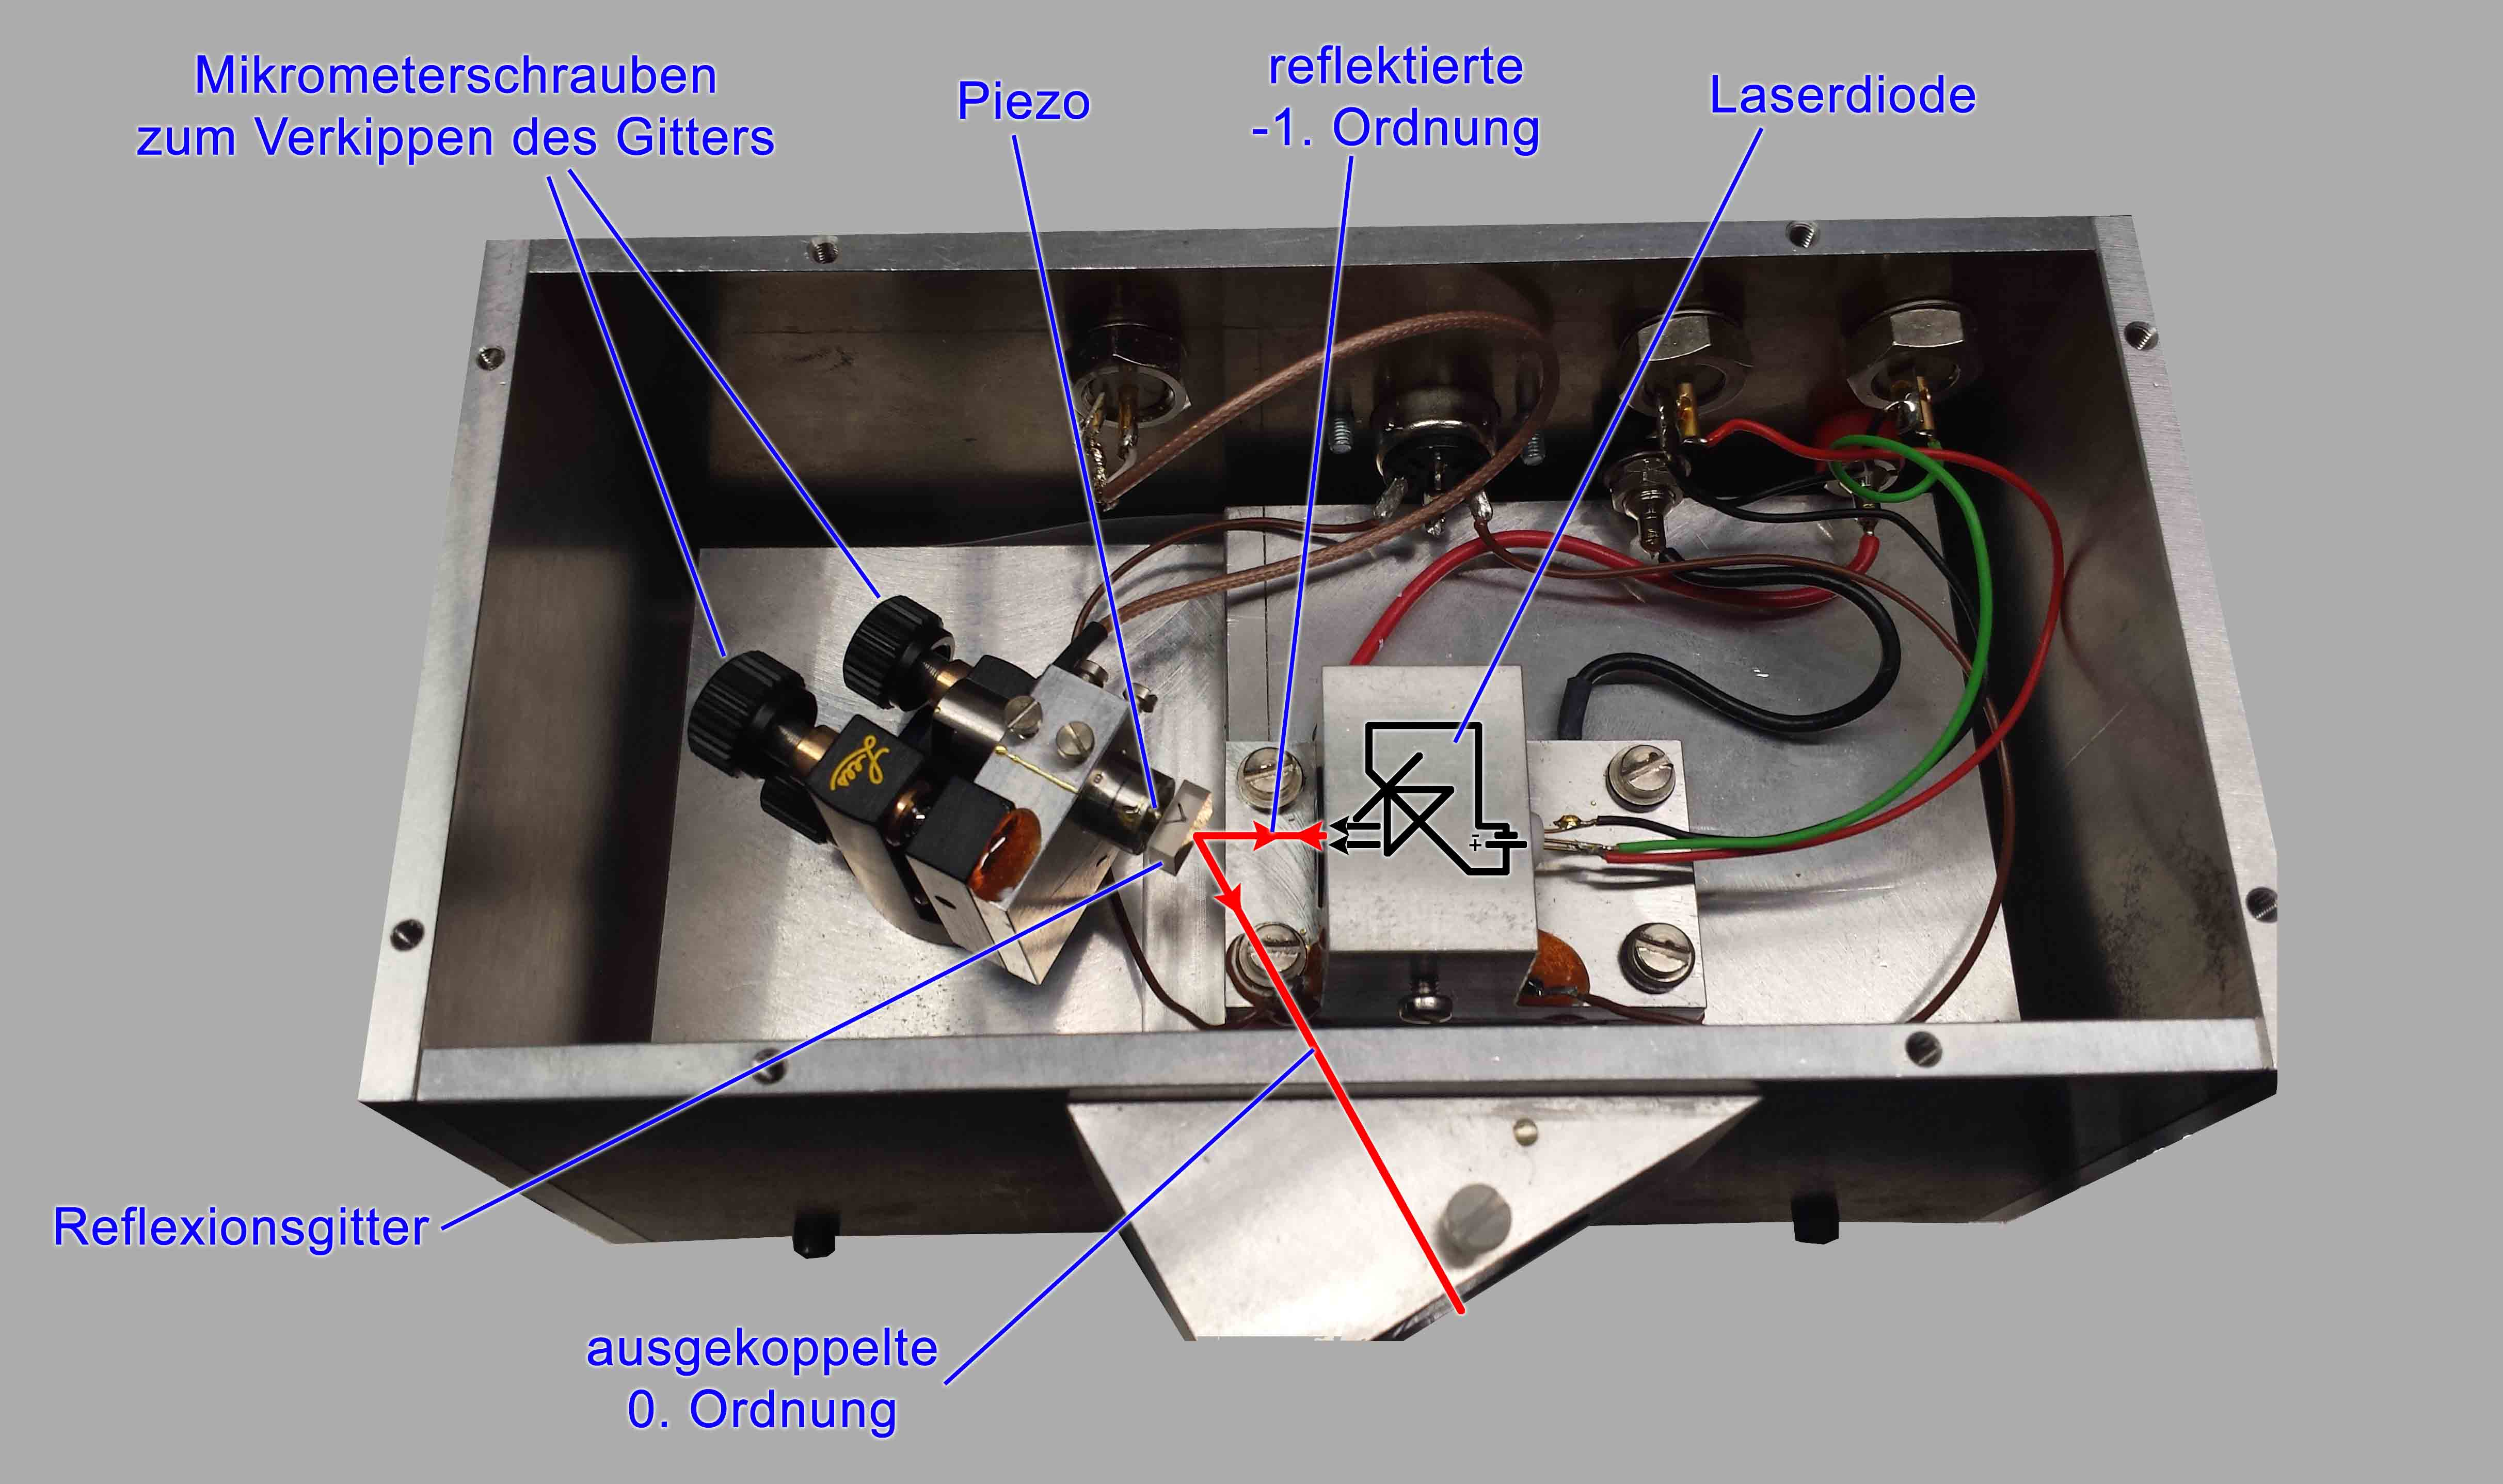
\includegraphics[width=480px]{Bilder/LLA2.jpg}
					\caption{Laser in Littrow Anordnung}
					\label{fig:LLA}
				\end{figure}
				
				\newpage
				
				\subsection{Dopplerfreie Sättigungsspektroskopie}
				
				Die Frequenz, auf welche der Rückpumplaser stabilisiert werden soll, muss, da es sich um eine absolute Stabilisierung handelt, klar definiert sein. Da der Laser einen atomaren Übergang von $^{85}$Rb anregen soll, liegt es nahe, mit Hilfe einer dopplerfreien Sättigungsspektroskopie einen atomaren Übergang von $^{85}$Rb als Referenz zu verwenden.\\
				Dazu wird ein Teil des Laserlichts durch eine mit Rubidiumdampf gefüllte Glaszelle gestrahlt und anschließend in sich selbst zurückreflektiert. Der Strahl trifft, nachdem er auf dem gleichen Weg durch die Glaszelle zurück gestrahlt wurde, auf eine Photodiode (siehe \autoref{fig:DSS}). Ist das Licht in seiner Frequenz gegenüber der Resonanz zu einem atomaren Übergang rotverstimmt (geringere Frequenz), so ``sehen'' Atome, die sich mit der entsprechenden Geschwindigkeit dem Licht entgegen bewegen aufgrund des optischen Dopplereffekts, eine Frequenz des Lichts, die
				der des Übergangs entspricht. Atome, die sich dem Strahl entgegen bewegen, können Photonen absorbieren. Aus der statistischen Verteilung der Bewegungsrichtung verschiedener Atome resultiert sowohl für den hinlaufenden als auch für den rücklaufenden Strahl Absorption. Analoges gilt für blauverstimmtes (höhere Frequenz) Licht.\\
				Hat das Licht jedoch die Resonanzfrequenz zu dem Übergang, so werden die Photonen nur von ruhenden Atomen absorbiert. Dies hat auf Grund der Lebensdauer des daraus entstehenden angeregten Zustands eine Sättigung des Übergangs zu Folge. Durch den hinlaufenden Strahl angeregte Atome können keine Photonen des rücklaufenden Strahls absorbieren. Wird der Frequenzbereich des Lasers durchgestimmt, so ergeben sich an den Stellen des Absorptionsspektrums, an denen das Licht resonant zu einem atomaren Übergang ist, Einbrüche in der Absorption, so genannte ``Lampdips''.\\
				Zur Stabilisierung des Lasers auf solch eine Resonanz wird das Absorptionssignal elektronisch abgeleitet. Dieses am Ausgang des Lock-in-Verstärkers anliegende (zur ersten Ableitung proportionale Signal), wird von der Regelbox (PID-Regler) zur Stabilisierung des Lasers verwendet. Dadurch kann die Frequenz der Laser auf einem solchen Lampdip ``gehalten'' werden.\\
				
				\begin{figure}[htb!]
					\centering
					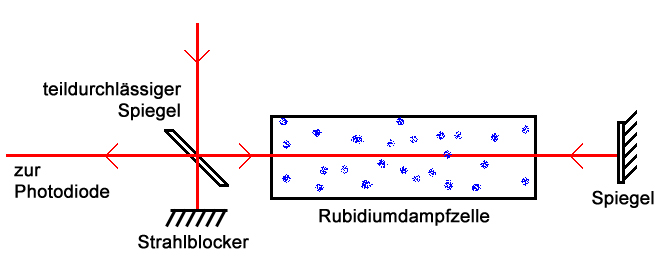
\includegraphics[width=320px]{Bilder/DSS.jpg}
					\caption{Schematische Skizze des Aufbaus einer dopplerfreien Sättigungsspektroskopie}
					\label{fig:DSS}
				\end{figure}
				
				\subsection{Offsetlock}\label{ssec:Offsetlock}
				
				Der Kühllaser wird über eine relative Stabilisierung zu dem Rückpumplaser auf seiner Frequenz gehalten. Dazu werden beide Strahlen überlagert und auf eine schnelle Photodiode fokussiert. Sind die beiden Laser nur um wenige GHz zueinander verstimmt, so kann auf der Diode ein Schwebungssignal der Intensität aufgenommen werden. Die Schwebung kann nun elektronisch aufgenommen und ausgewertet werden.
				%In Abbildung 2.4 ist die Spannung, die der Frequenz-zu-Spannungs-Wandler aus der Frequenz des Schwebungssignals erzeugt, in Abhängigkeit zur Spannung am Piezokristall des Kühllasers dargestellt. Verschiedene Spannungen entsprechen verschiedenen Emissionsfrequenzen des Lasers (der Rückpumplaser bleibt konstant). Auch dieses Signal kann zur Stabilisierung verwendet werden.
				Im Versuch ist ein Frequenz-zu-Spannungs-Wandler verbaut. Verschiedene Spannungen entsprechen verschiedenen Emissionsfrequenzen des Kühllasers (bei konstanter Frequenz des Rückpumplasers). Auch dieses Signal kann zur Stabilisierung verwendet werden.				
				
				\section{Theorie zur MOT}
				
				Die Idee, mit Licht Atome zu kühlen, wurde erstmals 1975 formuliert und schon im gleichen Jahr nachgewiesen.
				Eine magneto-optische Falle wurde 1987 erstmals realisiert und 1997 mit einem Nobelpreis ausgezeichnet. Zum
				Verständnis einer MOT kann ihre Funktionsweise in zwei Aspekte unterteilt werden: zum einen das Kühlen, zum
				anderen das Fangen der Atome.
				
				\subsection{Optisches Kühlen}
				
				Die Temperatur eines Ensembles von Atomen entspricht der gemittelten Bewegung der Atome. Da auf Grund der
				Erhaltung der Energie die Wärmeenergie $E_W = \frac{f}{2}k_BT$ der Bewegungsenergie $E_{kin} = \frac{1}{2}mv^2$ gleichgesetzt werden kann, folgt daraus, dass die Temperatur mit $T = mv^2/(k_Bf)$ quadratisch abhängig von der Geschwindigkeit ist.\\ 
				Soll ein atomares Ensemble gekühlt werden, muss die relative Geschwindigkeit der einzelnen Atome zueinander
				verringert werden. Im Falle der Laserkühlung nutzt man hierzu die Wechselwirkung zwischen Atomen und
				elektromagnetischer Strahlung definierter Richtung, Frequenz und Polarisation.
				
				\subsubsection{Spontankraft}\label{ssec:SK}
				
				Ein Photon, dessen Energie der Energiedifferenz zwischen zwei Energieniveaus in einem Atom entspricht, kann von diesem Atom absorbiert werden. Die Spontankraft entsteht durch stimulierte Absorption von Photonen aus einem Laserstrahl und anschließende spontane Reemission. Beim Absorptionsvorgang wird sowohl der Impuls $\vec{p} = \hbar \vec{k}$ als auch die Energie $E = \hbar \omega$ des Photons an das Atom weitergegeben, wobei $\vert \vec{k} \vert = 2\pi/\lambda$ die Wellenzahl und $v = \omega/2\pi$ die Frequenz des Photons ist. Nach einer für die Atomart spezifischen Lebensdauer $\tau$ werden die Photonen
				wieder unter spontaner Emission vom Atom abgegeben. Da der Impuls und die Energie Erhaltungsgrößen sind,
				sind ihre Beträge bei Absorption und Emission konstant. Das spontan emittierte Photon verleiht dem Atom einen Rückstoßimpuls. Die Wahrscheinlichkeit der Rückstoßrichtung ist über den gesamten Raum gleichverteilt. Somit mittelt sich die atomare Nettoimpulsänderung bei Emission statistisch zu Null.\\ Werden Photonen aus einer festen Richtung eingestrahlt, so addieren sich die Impulsüberträge bei Absorpion derart, dass eine gerichtete Kraft auf das Atom entsteht (siehe \autoref{fig:SK}).\\
				Zum Kühlen von Rubidiumatomen werden elektronische Übergänge im Atomspektrum verwendet. Diese können
				vereinfacht als atomare Zweizustandssysteme im elektromagnetischen Strahlungsfeld einer festen Frequenz
				betrachtet werden. Die Besetzungszustände können durch Absorption und spontane Reemission der Photonen des
				Strahlungsfeldes beeinflusst werden. Eine quantenmechanische Beschreibung dieses Modells in Form von Bewegungsgleichungen bieten die optischen Blochgleichungen. Unter Betrachtung des Gleichgewichtszustandes der in diesen Gleichungen beschriebenen Dynamik, lässt sich die Streurate $\varGamma_{sc}$ der Photonen des Strahlungsfeldes an einem Zweiniveauatom herleiten:
				
				\begin{equation}\label{equa:6-1}
				\varGamma_{sc} = \frac{\varGamma}{2} \frac{s_0}{1+s_0+(2\varDelta/\varGamma)^2}
				\end{equation}
				
				Hierbei ist $\varGamma$ die Zerfallsrate des angeregten Zustandes des Zweiniveausystems, $\varDelta = \omega_L - \omega_R $ ist die spektrale Verstimmung des Strahlungsfeldes der Frequenz $\omega_L$ gegenüber der atomaren Resonanz $\omega_R$ und $s_0$ ist der Sättigungsparameter im Falle der Resonanz. Er stellt das Verhältnis aus der Intensität des Lichtes \textit{I} und der Sättigungsintensität des atomaren Übergangs $I_0$ dar. Es gilt $s_0 = I/I_0$, wobei $I_0 = \pi hc\varGamma/(3\lambda^3)$.\\
				Wird das Licht aus einer festen Richtung auf ruhende Atome eingestrahlt, so ergibt sich unter Beachtung des bei jedem Streuvorgang auf das Atom übertragenen Photonenimpulses $\vec{p} = \hbar \vec{k}$ eine gerichtete Kraft, die Spontankraft $\vec{F}_D$
				
				\begin{equation}
				\vec{F}_D = \hbar \vec{k} \cdot \varGamma_{sc}
				\end{equation}
				
				Mit \autoref{equa:6-1} folgt
				
				\begin{equation}\label{equa:6-3}
				\vec{F}_D = \hbar \vec{k} \cdot \frac{\varGamma}{2} \frac{s_0}{1+s_0+(2\varDelta/\varGamma)^2}
				\end{equation}
				
				\begin{figure}[htb!]
					\centering
					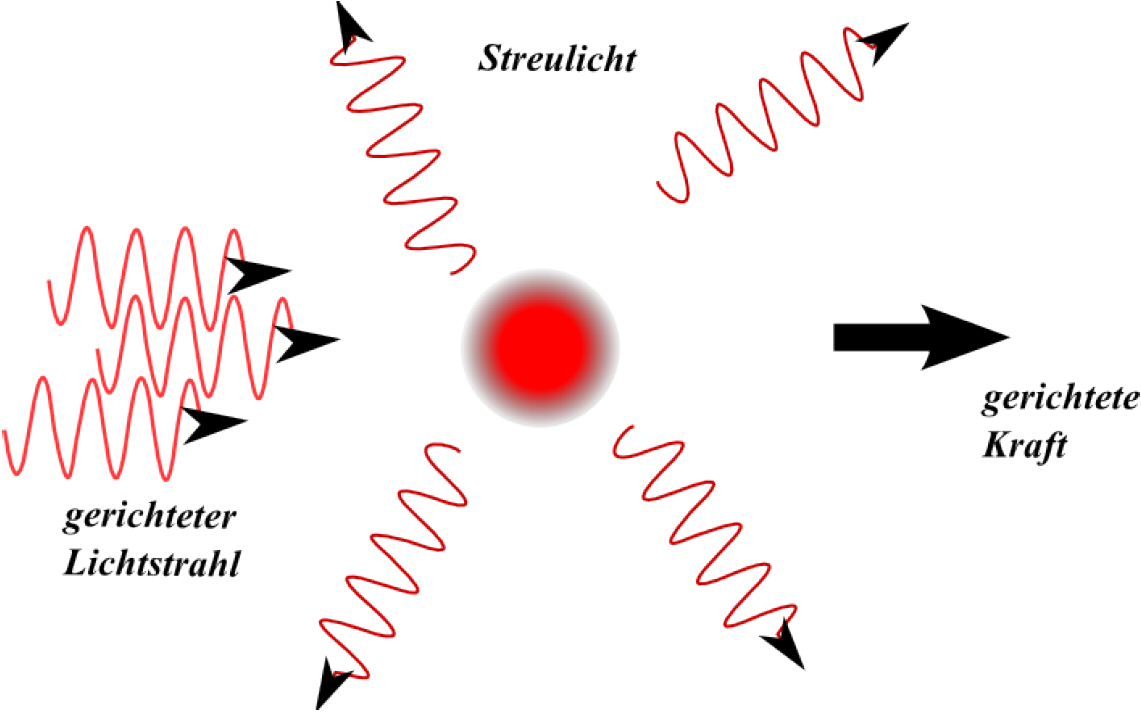
\includegraphics[width=350px]{Bilder/SK.jpg}
					\caption{Skizze zum Prinzip der Spontankraft}
					\label{fig:SK}
				\end{figure}
				
				\subsubsection{Dopplerkühlung - Optische Melasse}
				
				Um eine Kühlung eines atomaren Gases zu realisieren, muss die auf die Atome wirkende Kraft abhängig vom Betrag und Richtung der atomaren Geschwindigkeiten sein. Eine entsprechende Konfiguration des Lichtfeldes wird durch sechs aus allen Raumrichtungen kommenden, gegenüber der atomaren Resonanz rotverstimmten Laserstrahlen implementiert.\\
				Da die Kühlung entlang der drei Raumachsen voneinander unabhängig ist, wird der Einfachheit halber
				nur die Wirkung der Laserstrahlen in einer Dimension \textit{x} erläutert. Ergänzt wird die Betrachtung der Kraftausübung eines Laserstrahls auf Atome aus \autoref{ssec:SK} durch das Hinzuziehen eines weiteren, diesem Strahl entgegengerichteten Laserstrahls. Die auf ein Atom resultierende Gesamtkraft ergibt sich dann aus der Überlagerung der beiden in Richtung \textit{-x} und \textit{+x} wirkenden Kräfte $F_{x-}$ und $F_{x+}$ (aus \autoref{equa:6-3}) zu
				
				\begin{equation}
				F_{OM} = F_{x+} + F_{x-}
				\end{equation}
				
				mit
				
				\begin{equation}\label{equa:6-5}
				F_{x+\backslash x-} = \pm \hbar k \cdot \frac{\varGamma}{2} \frac{s_0}{1+s_0+(2\varDelta_{OM\pm}/\varGamma)^2} 
				\end{equation}
				
				Die Geschwindigkeitsabhängikeit der Kraft wird im Parameter
				
				\begin{equation}
				\varDelta_{OM\pm} = \varDelta \mp k v_{x}
				\end{equation}
				
				berücksichtigt, wobei $v_x$ die Geschwindigkeit der Atome in x-Richtung ist. Er korrigiert die Verstimmung des Lichtes um die Dopplerverschiebung, bedingt durch die Geschwindigkeit der Atome. Die Summe der beiden Kräfte ergibt sich nach Entwicklung für kleine Geschwindigkeiten unter Vernachlässigung der Terme ab der Ordnung $(kv/\varGamma)^4$ zu
				
				\begin{equation}\label{equa:6-7}
				F_{OM} = \frac{8 \hbar k^2 \varDelta s_0}{\varGamma (1+s_0 + (2\varDelta/\varGamma)^2)^2} v_x = -\beta v_x
				\end{equation}
				
				Ist das Licht rotverstimmt ($\varDelta < 0$), so sieht ein in positive x-Richtung fliegendes Atom das entgegenkommende Licht zur Resonanz hin dopplerverschoben, wobei die Wahrscheinlichkeit der Absorption eines Photons zunimmt.\\
				Es erfährt eine lineare rücktreibende Kraft ($\beta > 0$), die zur Abbremsung führt. Die Kraft auf das Teilchen ist genau dann maximal, wenn die Verstimmung des Lasers die Dopplerverschiebung kompensiert: $\varDelta = k v_x$ .
				Wegen der Analogie des Abbremsvorgangs (\autoref{equa:6-7}) zur viskosen Dämpfung in einer nahen Umgebung
				von $v_x = 0$, wird dieser Prozess \textit{optische Melasse} genannt. Auf Grund der zentralen Bedeutung des Dopplereffektes bei dieser Art von Kühlung spricht man von $Doppler-Kühlung$. Die Temperatur der optischen Melasse ergibt sich aus dem Gleichgewicht aus Dopplerkühlung und Aufheizen des Ensembles durch die remittierten Photonen.\\ 
				Die minimal erreichbare Temperatur, die mittels der Dopplerkühlung erreicht werden kann, das so genannte
				Dopplerlimit, beträgt
				
				\begin{equation}
				T_D = \frac{\hbar \varGamma}{2 k_B}.
				\end{equation}
				
				\begin{figure}[htb!]
					\centering
					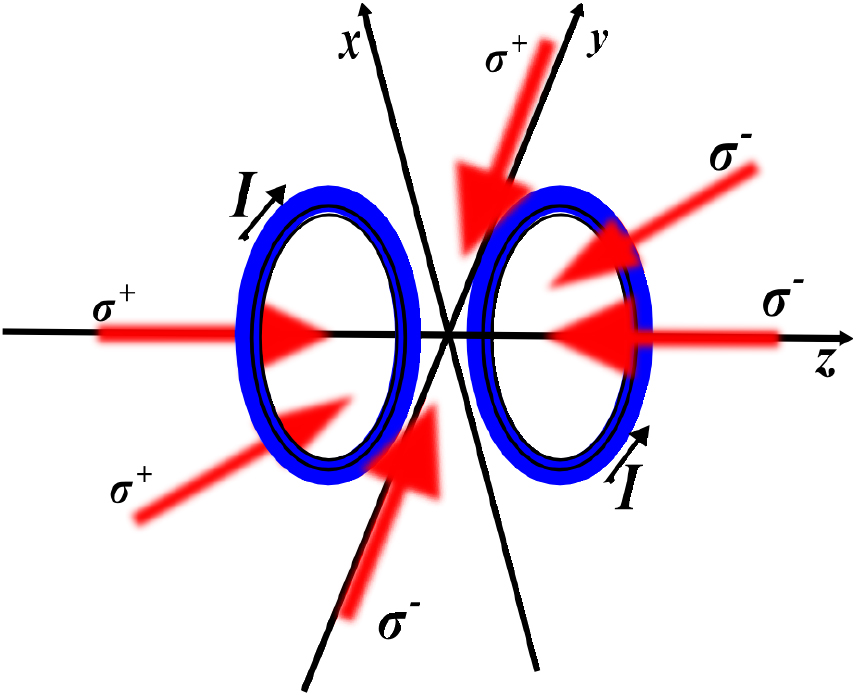
\includegraphics[width=350px]{Bilder/MOTSS.jpg}
					\caption{Schematische Skizze der MOT: Durch das Spulenpaar wird ein Quadrupolfeld induziert, das im Mittelpunkt der MOT - dem Schnittpunkt der drei senkrecht zueinander stehenden Strahlenpaare - Null
						ist. Jedes antiparallele Strahlenpaar besteht aus einem $\sigma^+$- und einem $\sigma^-$-polarisierten Strahl.}
					\label{fig:MOTSS}
				\end{figure}
				
				\subsection{Fangen der Atome}
				
				Mit dem oben beschriebenen Verfahren lassen sich Atome kühlen. Jedoch stellt es noch keine Falle für Atome dar. Teilchen werden zwar im Impulsraum gefangen, haben aber im Ortsraum volle Bewegungsfreiheit, so dass sie nach einer gewissen Zeit aus der optischen Melasse herausdiffundieren können. Um Atome zu fangen, wird der oben beschriebene rotverstimmten Strahlenkonfiguration in ihrem Schnittpunkt ein inhomogenes magnetisches Feld überlagert (siehe \autoref{fig:MOTSS}). Dieses Feld (Quadrupolfeld) wird durch zwei stromdurchflossene Spulen in Anti-Helmholtz-Konfiguration erzeugt. Das Prinzip der so erzeugten MOT wird nachfolgend in einer Dimension \textit{x} anhand eines atomaren Übergangs von einem Grundzustand $\lvert \phi_{n,F=0,m_F}\rangle$ in einen angeregten Zustand $\lvert \phi_{n,F'=1,m_{F'}}\rangle$ erklärt.
				\textit{n} ist hierbei die Hauptquantenzahl, \textit{F} bzw. \textit{F'} ist der Gesamtdrehimpuls des entsprechenden Zustandes und $m_F$ bzw. $m_{F'}$ die dazugehörige magnetische Quantenzahl. Diese hat für den Zustand $\lvert \phi_{n,F=0,m_F}\rangle$ den Wert $m_F=0$ und für den Zustand $\lvert \phi_{n,F'=1,m_{F'}}\rangle$ die Werte $m_F \in \{-1,0,1\}$. Zur Erklärung des Mechanismus muss die Polarisation der Strahlen, welche zirkular ist, mitbetrachtet werden.\\
				Das durch die Spulen hervorgerufene Quadrupolfeld kann in der Fallenmitte linearisiert und mit der Gleichung
				
				\begin{equation}
				B_x = B(x) = B_0 \cdot x
				\end{equation}
				
				beschrieben werden, wobei $B_0$ der Gradient des Magnetfeldes in x-Richtung ist. Durch den Zeemaneffekt wird innerhalb des Zustandes $\lvert \phi_{n,F'=1,m_{F'}}\rangle$ eine energetische Aufspaltung der drei magnetischen Unterzustände $m_{F'}$ um den Term $\varDelta E$ hervorgerufen:
				
				\begin{equation}
				\varDelta E = g_{F'} m_{F'} \mu_B B_x
				\end{equation}
				
				Hierbei ist $\mu_B = e \hbar / 2 m_e$ das Bohrsche Magneton mit der Elektronenmasse $m_e$ und $g_{F'}$ der Landé-Faktor des Zustands $\lvert \phi_{n,F'=1,m_{F'}}\rangle$. \autoref{fig:FA} zeigt die Falle. Bewegt sich ein Atom aus der Fallenmitte heraus, so wird je nach Bewegungsrichtung der Zustand $m_{F'} = \pm 1$ energetisch abgesenkt, so dass die atomare Resonanz zur eingestrahlten Lichtfrequenz hin verschoben wird. Fliegt bespielsweise ein Atom in positive x-Richtung, so steigt die Wahrscheinlichkeit der Absorption eines $\sigma^-$-Photons, welches einen elektronischen Übergang in den Zustand $m_{F'} = -1$ induziert. Da dieses Photon in negative x-Richtung fliegt, erfährt das Teilchen einen Rückstoß in Richtung
				Fallenmitte. Ensprechend verhält es sich mit Teilchen, die in die entgegengesetzte Richtung propagieren.
				Durch diesen Mechanismus, der sowohl im Impuls-, als auch im Ortsraum wirkt, wird sowohl eine Kühlung, als
				auch eine Verdichtung der Atome erreicht. Die in \autoref{equa:6-5} hergeleitete Kraft wird ortsabhängig:
				
				\begin{equation}\label{equa:6-11}
				F_{x+\backslash x-} = \pm \hbar k \cdot \frac{\varGamma}{2} \frac{s_0}{1+s_0+(2\varDelta_{OM\pm}/\varGamma)^2} 
				\end{equation}
				
				wobei
				
				\begin{equation}
				\varDelta_{OM\pm} = \varDelta \mp k v_{x} \pm \frac{g_{F'} m_{F'} \mu_B B_0 x}{\hbar}
				\end{equation}
				
				gilt. Wird dies in $F_{MOT} = F_{x_+} + F_{x_-}$ eingesetzt und entwickelt unter der Annahme, die Teilchen hätten kleine Geschwindigkeiten und befänden sich nahe der Fallenmitte, so lässt sich unter Vernachlässigung höherer Ordnungen, vereinfacht schreiben:
				
				\begin{equation}\label{equa:6-13}
				F_{MOT} = -\beta v_x  -\kappa x
				\end{equation}
				
				mit $\beta$ wie in \autoref{equa:6-7} und $\kappa = \frac{g_{F'} m_{F'} \mu_B B_0}{\hbar k}$. \autoref{equa:6-13} zeigt, dass sich die Teilchen im MOT-Betrieb wie gedämpfte harmonische Oszillatoren verhalten.\\
				
				\begin{figure}[htb!]
					\centering
					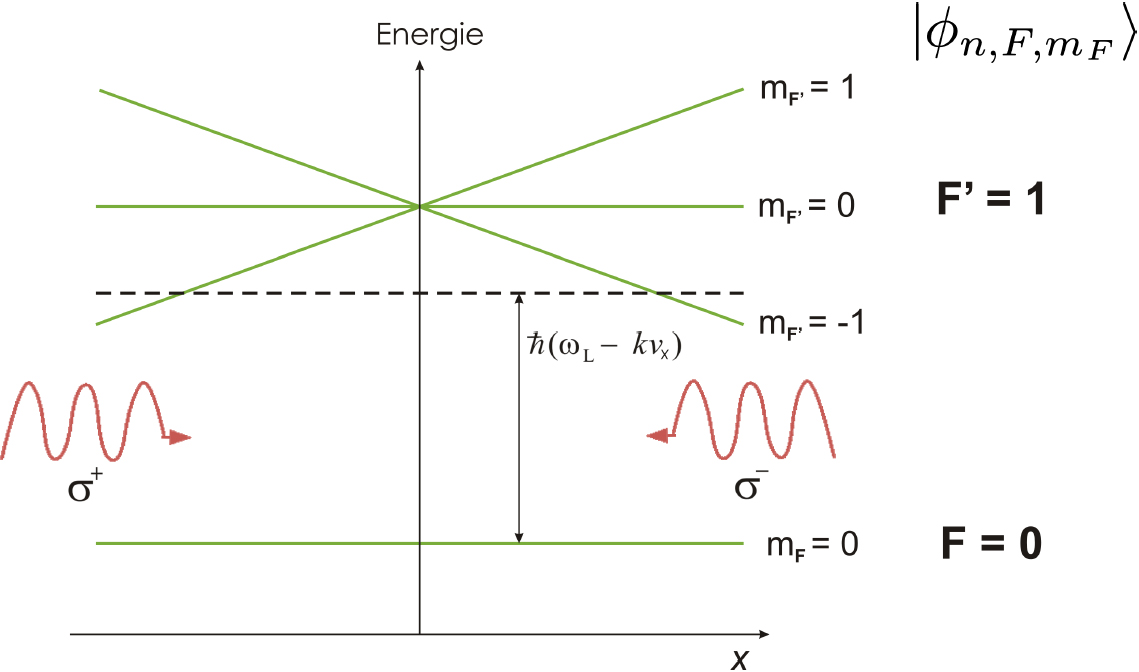
\includegraphics[width=350px]{Bilder/FA.jpg}
					\caption{Durch Anlegen eines Magnetfeldes spaltet der angeregte Zustand auf. Für das rotverstimmte Kühllicht ($\omega_L$) ist die Resonanzgbedingung erfüllt, wenn die Atome weit genug von der Fallenmitte entfernt sind. Sie ist auf Grund der Dopplerverschiebung (-kv) ebenfalls auch für Atome mit hohen Geschwindigkeiten erfüllt. Die Absorption der Photonen bewirkt eine Kraft in Richtung Fallenmitte.}
					\label{fig:FA}
				\end{figure}
				
				\fbox{\parbox[c]{17,2cm}{
						\begin{frage}\label{f4-1}
							Welche Aufbaukomponenten werden zur Erzeugung einer MOT benötigt? Wo wird das Licht in die drei Strahlen aufgeteilt? Wie verlaufen die Strahlen?
						\end{frage}
					}}\\
					
					\subsection{Rubidium-MOT}
					
					Bei Rubidium handelt es sich um ein Alkalimetall, welches verschiedene Isotope besitzt. Das im Versuch verwendete stabile Isotop ist $^{85}$Rb. Aus diesem Grund soll auf dessen Termschema kurz etwas genauer eingegangen werden.\\
					Für den Versuch spielt insbesondere die Aufspaltung des Energieniveaus in die Fein- und Hyperfeinstruktur eine zentrale Rolle (siehe \autoref{fig:TS}).\\
					Um sich die Aufspaltung in die Fein- beziehungsweise Hyperfeinstruktur herzuleiten ist es zudem noch wichtig zu wissen, dass $^{85}$Rb einen Kernspin von I=5/2 besitzt.\\ 
					Die verwendeten Übergänge zur Laserstabilisierung bzw. zur Anregung der Atome befinden sich zwischen dem $5^2S_{1/2}$ und dem $5^2P_{3/2}$ Niveau beziehungsweise deren Unterniveaus der Hyperfeinstruktur. Dies entspricht einer Wellenlänge von circa 780nm.\\
					Der in \textcolor{red}{rot} eingezeichnete Übergang a) von F=2 nach F'=1 wird zur Stabilisierung des Rückpumplasers verwendet. Allerdings muss hierbei beachtet werden, dass durch den AOM eine Frequenzverschiebung um 96MHz (Blauverstimmung) stattfindet, sodass die Frequenz des Rückpumplasers nach Durchlaufen des AOMs der Frequenz des Übergangs von F=2 nach F'=3 (Übergang b)) entspricht, der als Rückpumpübergang verwendet werden soll.\\
					Als Kühlübergang wird der Übergang von F=3 nach F'=4 verwendet (Übergang c)). Dessen Verstimmung in Bezug auf den Rückpumplaser kann entsprechend der Energiedifferenz zwischen Übergang b) und c) vor dem AOM eingestellt werden (2915MHz Rotverstimmung), da dieser beim Durchlaufen des AOMs die gleiche Frequenzverschiebung erfährt.\\   
					Die Auswahl der Übergänge erscheint zunächst etwas willkürlich. Macht man sich jedoch klar, dass für die erfolgreiche Realisierung der MOT ein Zweiniveausystem ideal ist, legitimiert dies die Auswahl der Übergänge, da man durch diese einem Zweiniveausystem am nächsten kommt.\\
					Betrachtet man als Erweiterung nun noch die Aufspaltung in die $m_F$ Niveaus gleicher Energie (siehe \autoref{fig:TS}), so sieht man, dass bei Anregung durch $\sigma^-$- oder $\sigma^+$-Licht nach wenigen Absorbtions- und Emissionsprozessen auch hier eine Festlegung in Richtung eines Zweiniveausystems stattfindet.\\  
					Dies kann man sich anhand der Auswahlregeln für Dipolstrahlung überlegen. Vom F'=4 Niveau kann gemäß $\varDelta F=0,\pm1$ nur ein Zerfall nach F=3 stattfinden. Da jedoch der Laser eine endliche Linienbreite hat, existiert eine von  Null verschiedene Wahrscheinlichkeit, dass beim Kühlübergang ein Atom in den F'=3 Zustand gelangt, von welchem ein Zerfall nach F=2 möglich ist. Um also sowohl einen günstigen Anfangszustand herzustellen und diesen auch beizubehalten wird der Rückpumplaser benötigt, um die Atome wieder in das F=3 Niveau zu bringen.\\
					Um die nun betrachteten Übergänge jedoch in Einklang mit dem Spektroskopiesignal zu bringen, muss ein weiterer Effekt beachtet werden. Bei diesem handelt es sich um sogenannte Crossover-Resonanzen. Diese treten auf, wenn sich die Frequenz des Laserlichtes gerade zwischen zwei oberen Energieniveaus befindet. Dies ist in \autoref{fig:TS} durch den \textcolor{green}{grünen} Pfeil dargestellt.\\
					Bei dieser Anregungsfrequenz ``sehen'' Atome, die sich dem Sättigungsstrahl beispielsweise entgegen bewegen, eine Frequenz die dem Übergang  von F=2 nach F'=3 entspricht und werden angeregt. Für den zurücklaufenden Probestrahl bewegen sich diese angeregten Atome gerade vom Strahl weg und so entspricht die Frequenz durch die Dopplerverschiebung der Übergangsfrequenz von F=2 nach F'=2. Da die Atome aber bereits angeregt sind kommt es wiederum zu einem Einbruch der Absorption und es entsteht ein weiterer Lambdip.\\
					Ein solches Sättigungsspektrum kann \autoref{fig:COF} (von F=2 nach F' für $^{85}$Rb) entnommen werden.\\ 
					
					
					\begin{figure}[htb!]
						\centering
						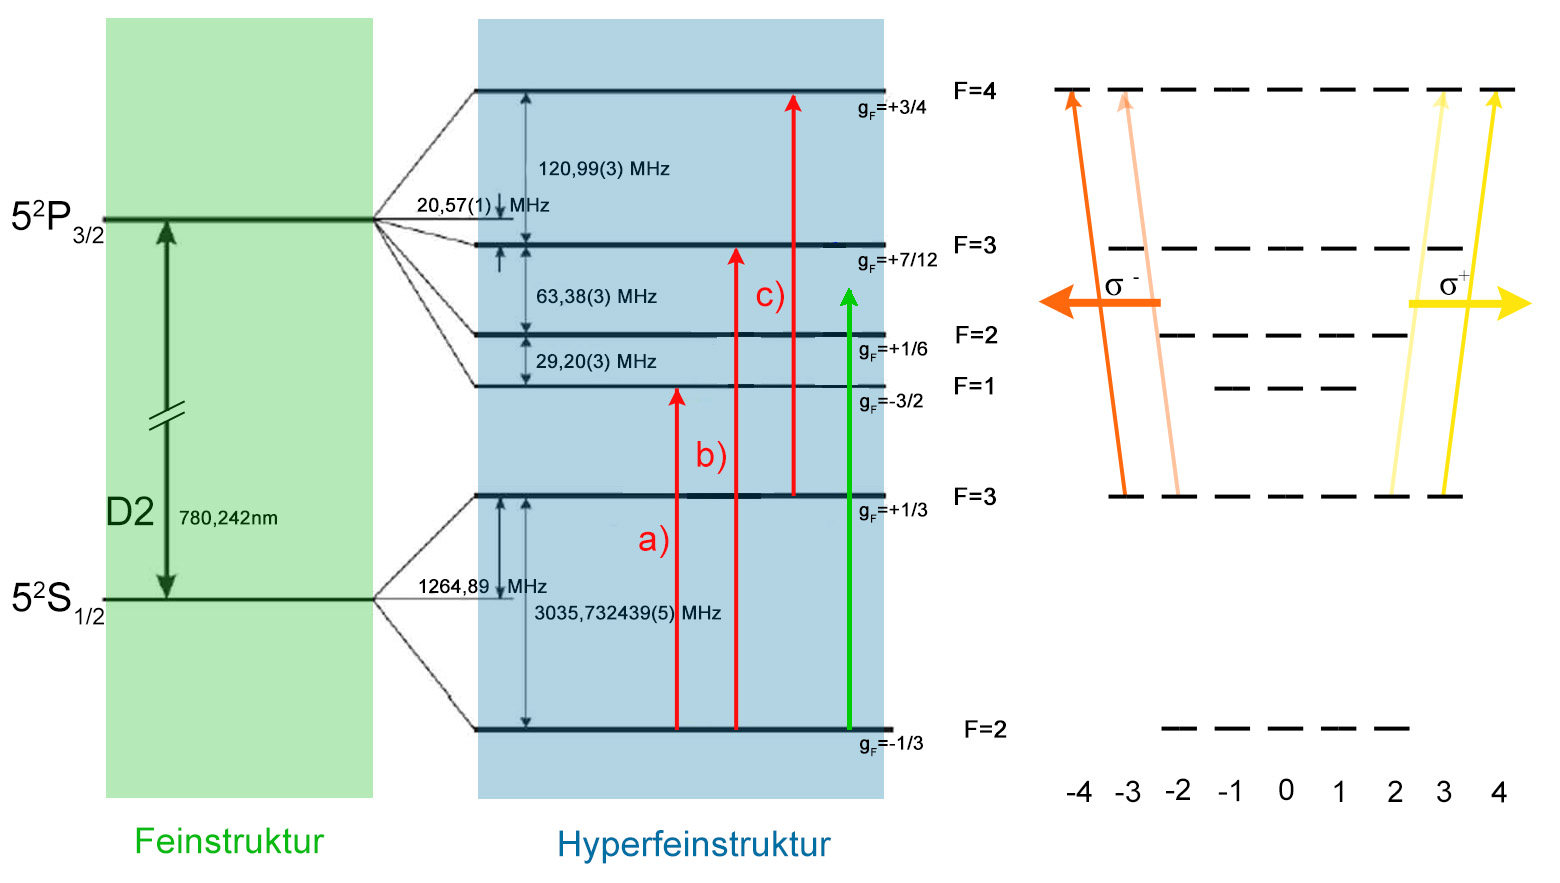
\includegraphics[width=480px]{Bilder/TS_korrigiert.jpg}
						\caption{Ausschnitt aus dem Termschema von $^{85}$Rb (D2-Linie) mit entsprechenden Übergangsfrequenzen}
						\label{fig:TS}
					\end{figure}
					
					
					\begin{figure}[htb!]
						\centering
						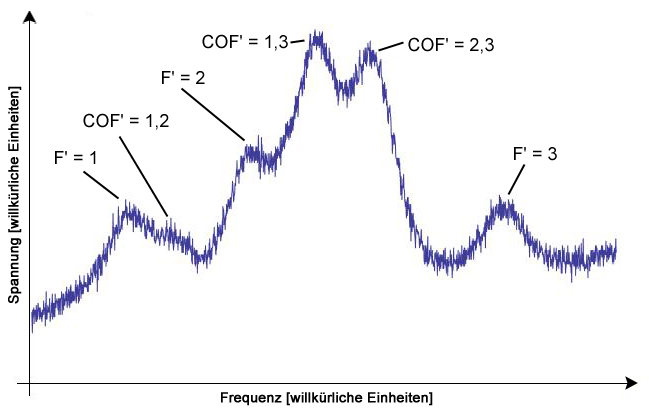
\includegraphics[width=480px]{Bilder/SCO.jpg}
						\caption{Spektroskopiesignal mit markierten Übergängen (F' für normale Übergänge und COF' für Crossover-Resonanzen)}
						\label{fig:COF}
					\end{figure}
					
					
					\newpage
					
					\section{Fragenkatalog}\label{sec:FK}
					
					\subsection{Vorbereitungsfragen}
					
					\begin{itemize}
						\item \textbf{Frage 4.1:} Welchen Vorteil bietet es, den Aufbau der MOT durch ein Glasfaserkabel von dem Aufbau der Laserstabilisierung zu trennen?
						
						\item \textbf{Frage 5.1:} Inwiefern ist die durch den AOM verursachte Frequenzverschiebung des Laserlichts in Bezug auf die Stabilisierung des Rückpump- und Kühllasers bzw. die an der MOT benötigte Frequenz relevant?
						
						\item \textbf{Frage 5.2:} Zu welchem Zweck werden die in den schematischen Skizzen zur Laserstabilisierung und der MOT eingezeichneten Verzögerungsplatten jeweils verwendet?
						
						\item \textbf{Frage 5.3:} Zu welchem Zweck werden die PST verwendet und warum kommen sie stets in Kombination mit einer $\lambda/2$-Platte vor? 
						
						\item \textbf{Frage 6.1:} Durch welche Größen/Faktoren werden die Laserfrequenzen beeinflusst? Welche dieser Faktoren sind gewollt beziehungsweise ungewollt und wie können diese beseitigt werden?
						
						\item \textbf{Frage 7.1:} Welche Elemente werden zur Erzeugung einer MOT benötigt? Wo wird das Licht in die drei Strahlen aufgeteilt? Wie verlaufen die Strahlen?
					\end{itemize}
					
					\subsection{Fakultative Fragen zum Selbsttest}
					
					\begin{itemize}
						\item Zur Aufnahme der Signale: Wie funktioniert die Triggerung eines Oszilloskopes und was bewirken die Kanaleinstellungen AC bzw. DC? 
						
						\item Beschreiben Sie den Aufbau des Lasersystems. Welche Funktion haben die einzelnen Elemente? Wo befinden sich die Elemente zur Stabilisierung der Laser? 
						
						\item Wo kann das Licht geschaltet werden?
						
						\item Welche Stabilisierungstechniken werden verwendet und wie funktionieren diese?
						
						\item Wie ist es möglich, die Laserfrequenz für die Spektroskopie kontrolliert durchzustimmen?
						
						\item Welche Möglichkeiten gibt es für die Aufnahme einer Messreihe zur Temperaturbestimmung?
						
						\item Welche Funktionen erfüllen die Elemente der MOT und warum werden diese benötigt, um Atome zu fangen?
						
						\item Welcher Temperatur entspricht das Dopplerlimit für $^{85}$Rb?
						
						\item Auf welchem Prinzip beruht die sogenannte Sub-Dopplerkühlung und welche Möglichkeiten eröffnet diese?
						
						\item Welche Übergänge von $^{85}$Rb werden zur Laserstabilisierung beziehungsweise zum Kühlen der Atome verwendet und warum ist dies sinnvoll?
						
						\item Welche natürliche Linienbreite und Lebensdauer ist für die D2-Linie von $^{85}$Rb charakteristisch?
						
						\item Welche Verstimmung des Laserlichts ist zum Kühlen der Atome ideal und welchen Wert muss diese für $^{85}$Rb annehmen?
						
						
					\end{itemize}
					
					
					
					
					\newpage
					
					\appendix
					
					\section{Anhang}
					
					\subsection{Fotos des Versuchsaufbaus}
					
					\begin{figure}[htb!]
						\centering
						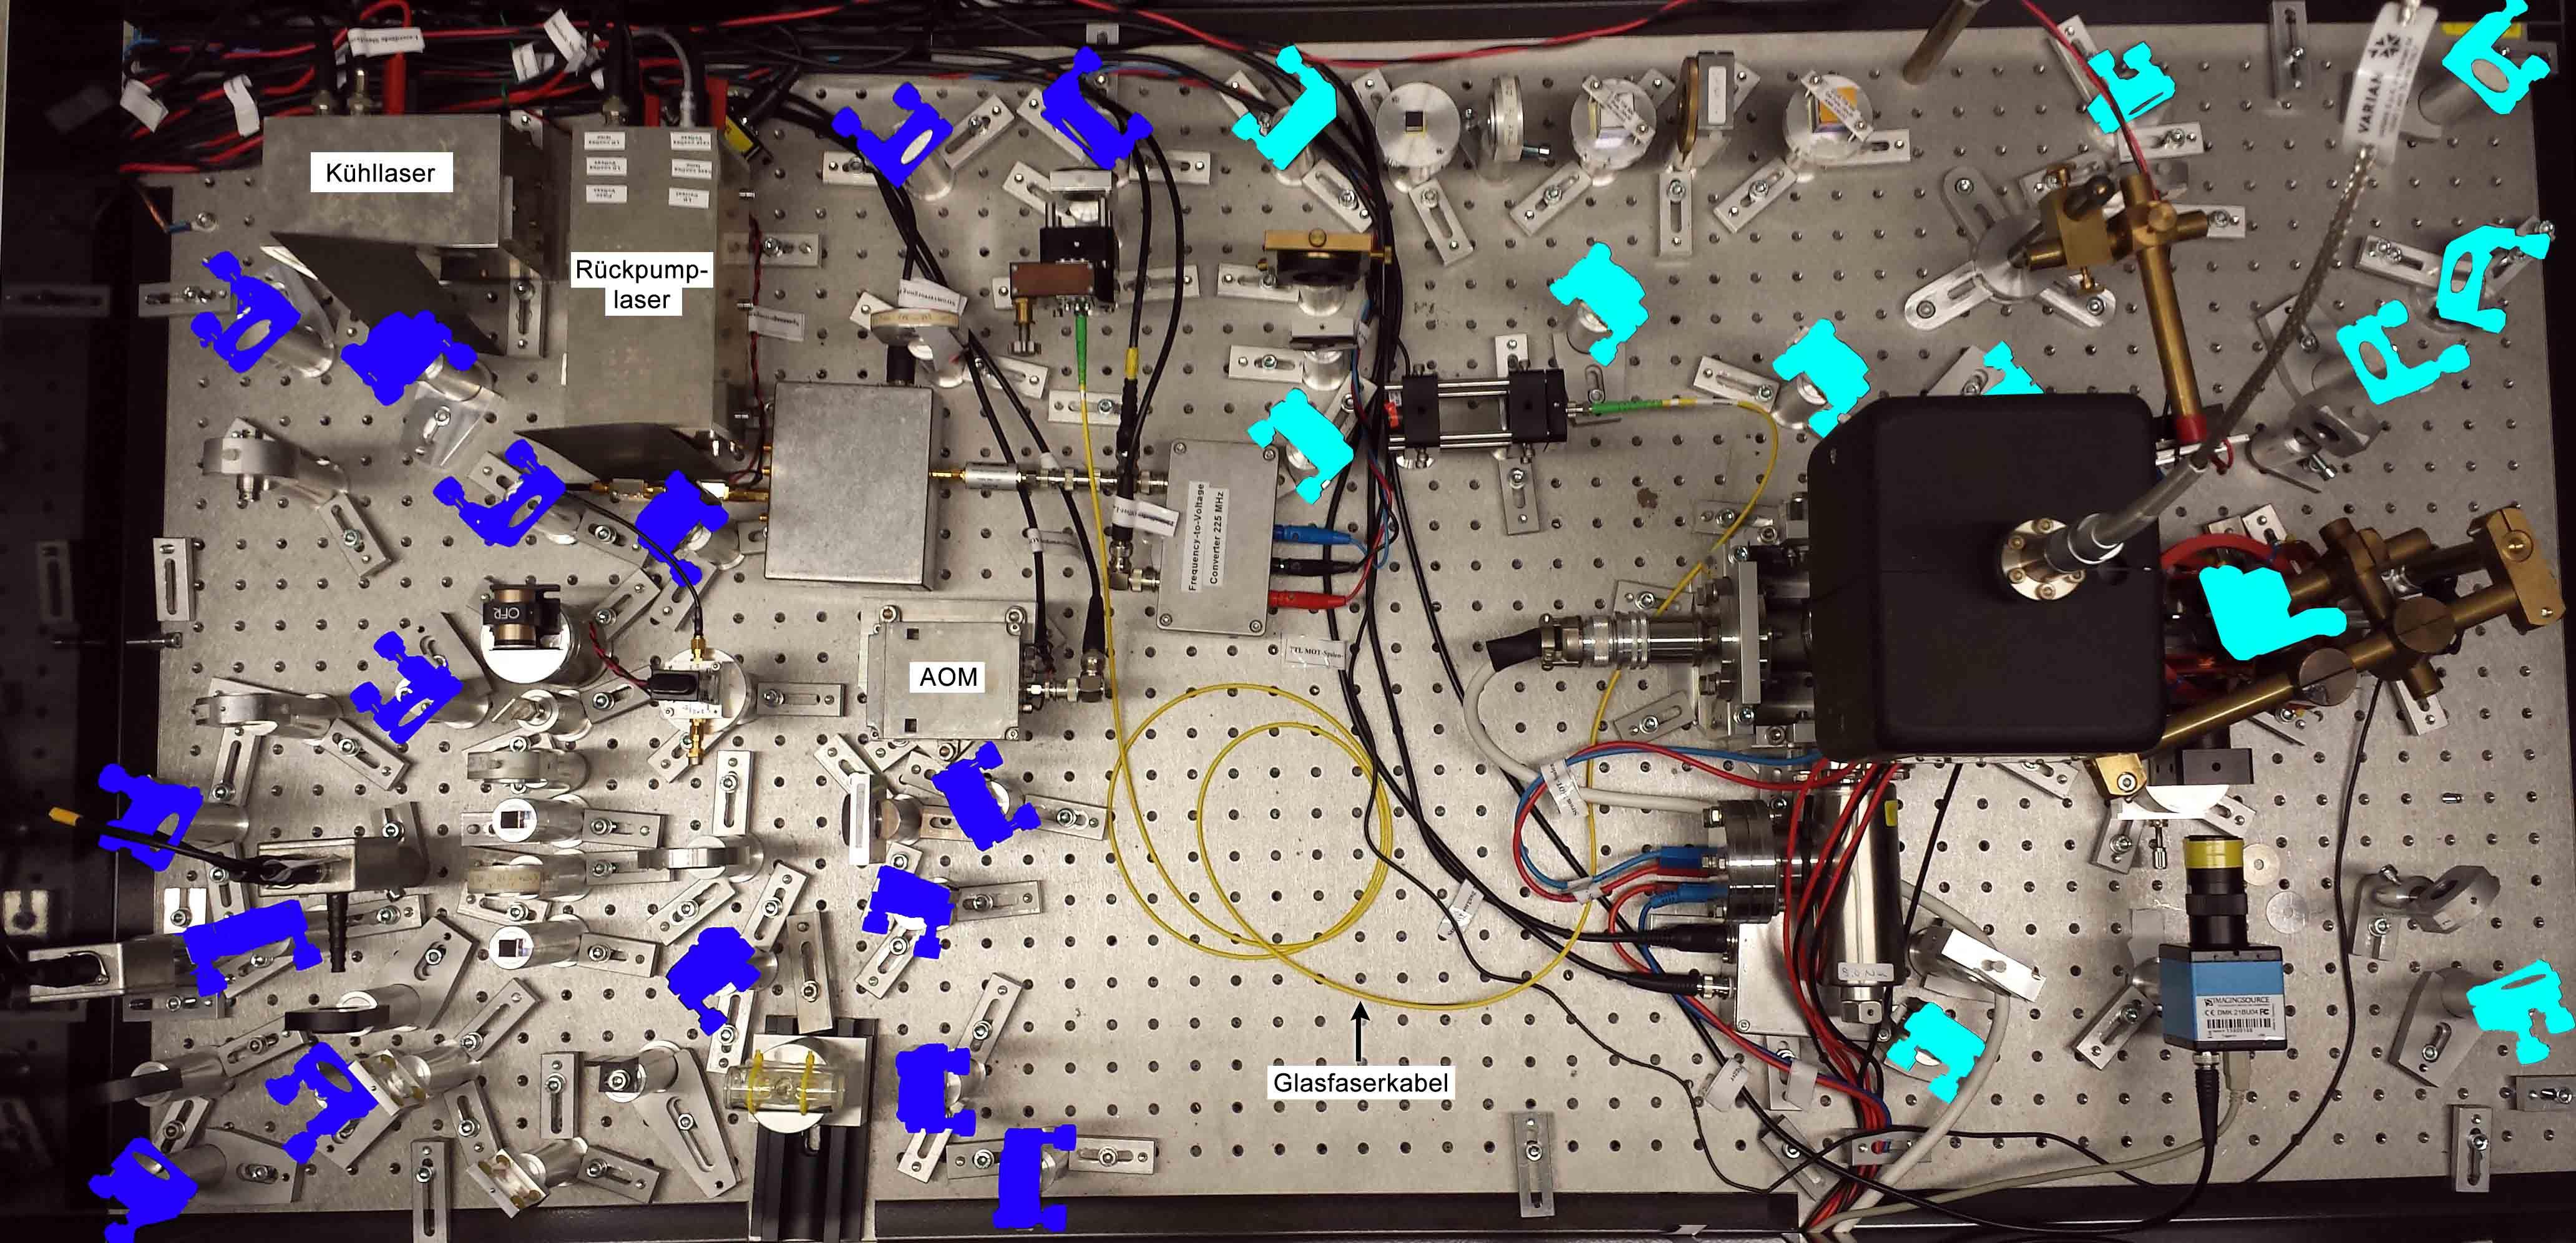
\includegraphics[width=480px]{Bilder/SL.jpg}
						\caption{\textcolor[cmyk]{0.86,0.77,0,0}{Spiegel der Laserstabilisierung} und \textcolor[cmyk]{0.52,0,0.16,0}{Spiegel der MOT}}
						\label{fig:SL}
					\end{figure} 
					
					~\\
					~\\
					~\\
					
					
					\begin{figure}[htb!]
						\centering
						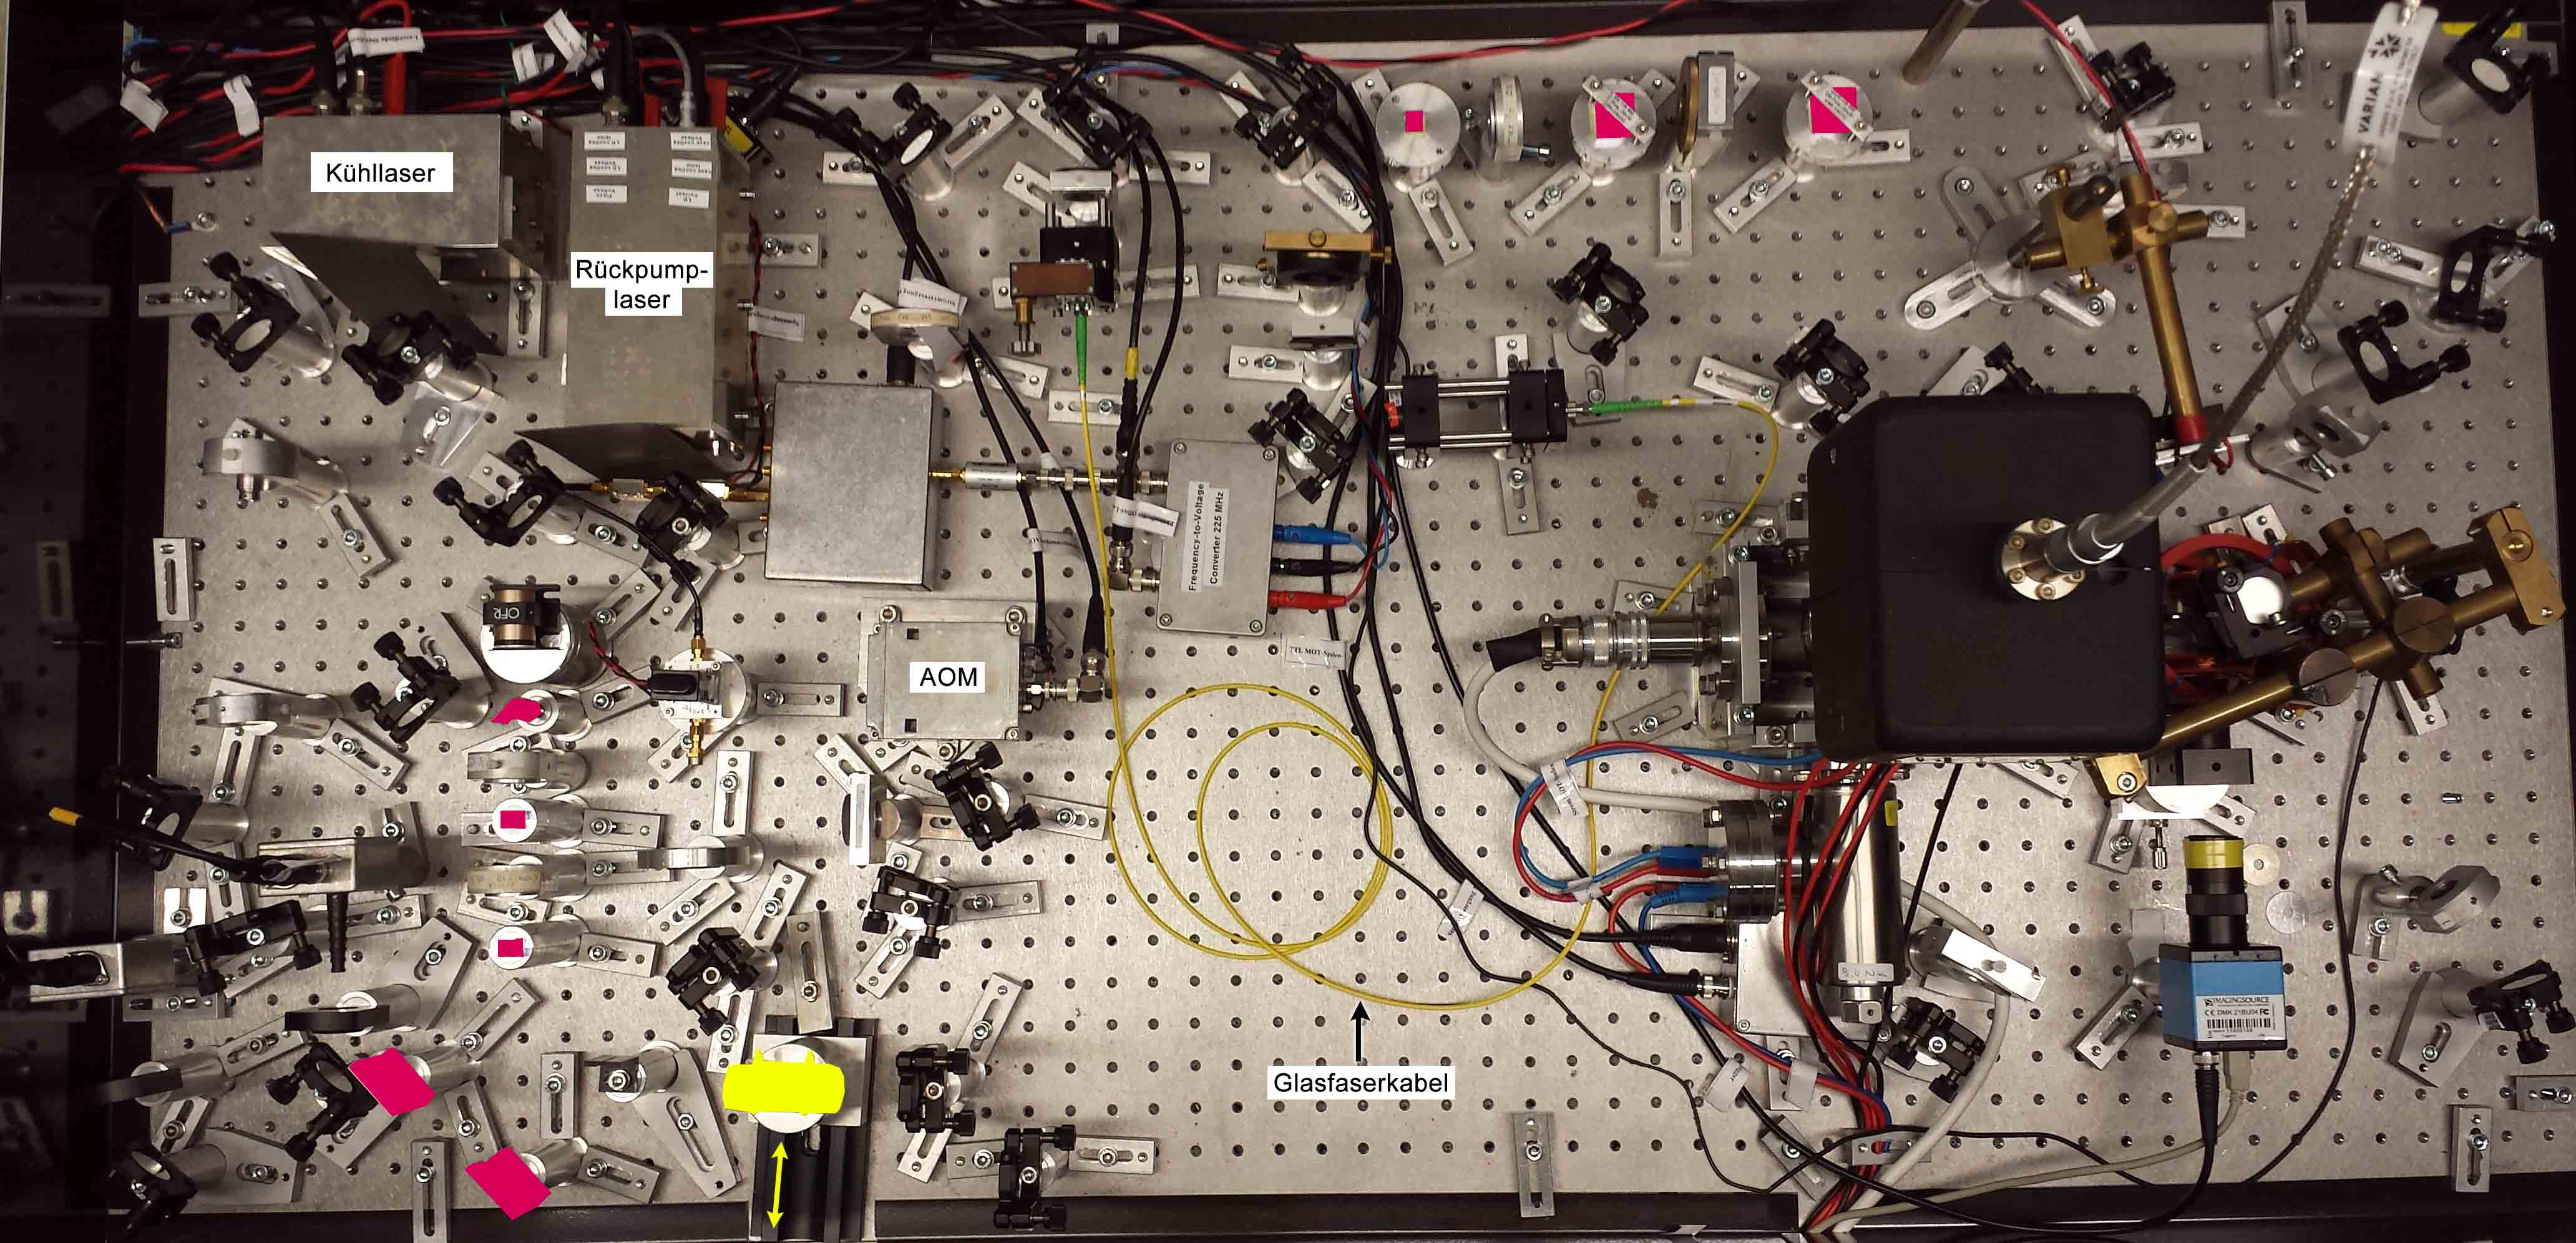
\includegraphics[width=480px]{Bilder/ST.jpg}
						\caption{\textcolor[cmyk]{0.11,1,0.47,0.01}{Strahlteiler} und \textcolor[cmyk]{0.1,0,0.99,0}{Rubidiumdampfzelle}}
						\label{fig:SW}
					\end{figure} 
					
					
					\begin{figure}[htb!]
						\centering
						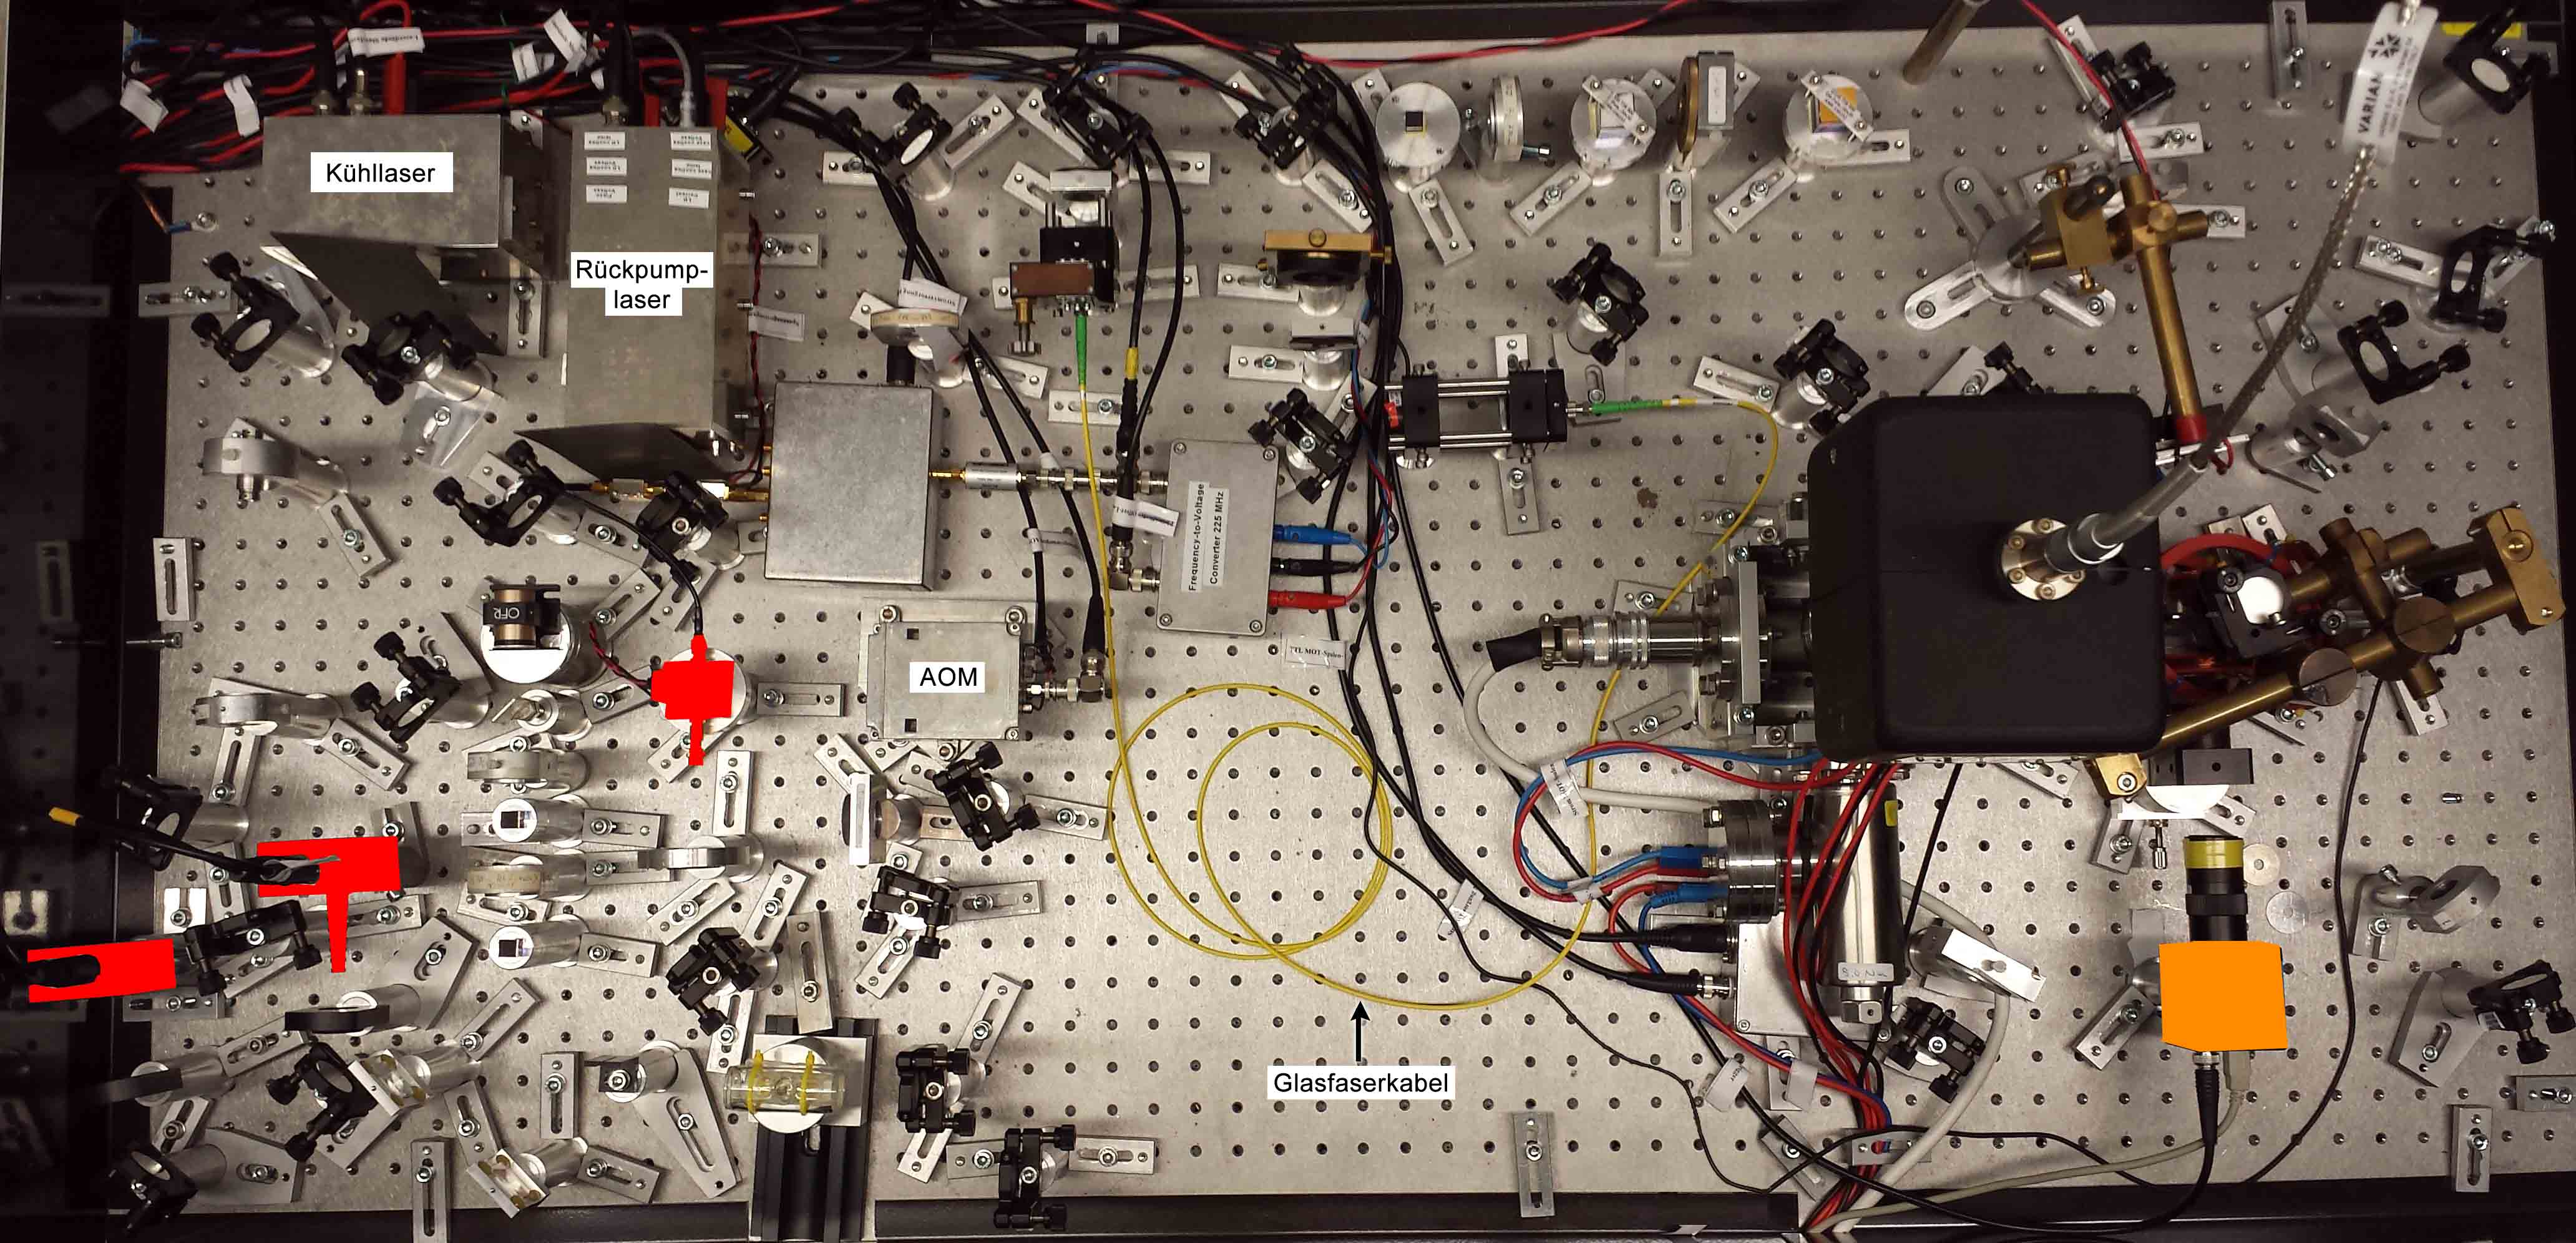
\includegraphics[width=480px]{Bilder/PDUK.jpg}
						\caption{\textcolor[cmyk]{0,0.99,1,0}{Photodioden} und \textcolor[cmyk]{0,0.56,1,0}{USB-Kamera}}
						\label{fig:PD}
					\end{figure}
					
					\begin{figure}[htb!]
						\centering
						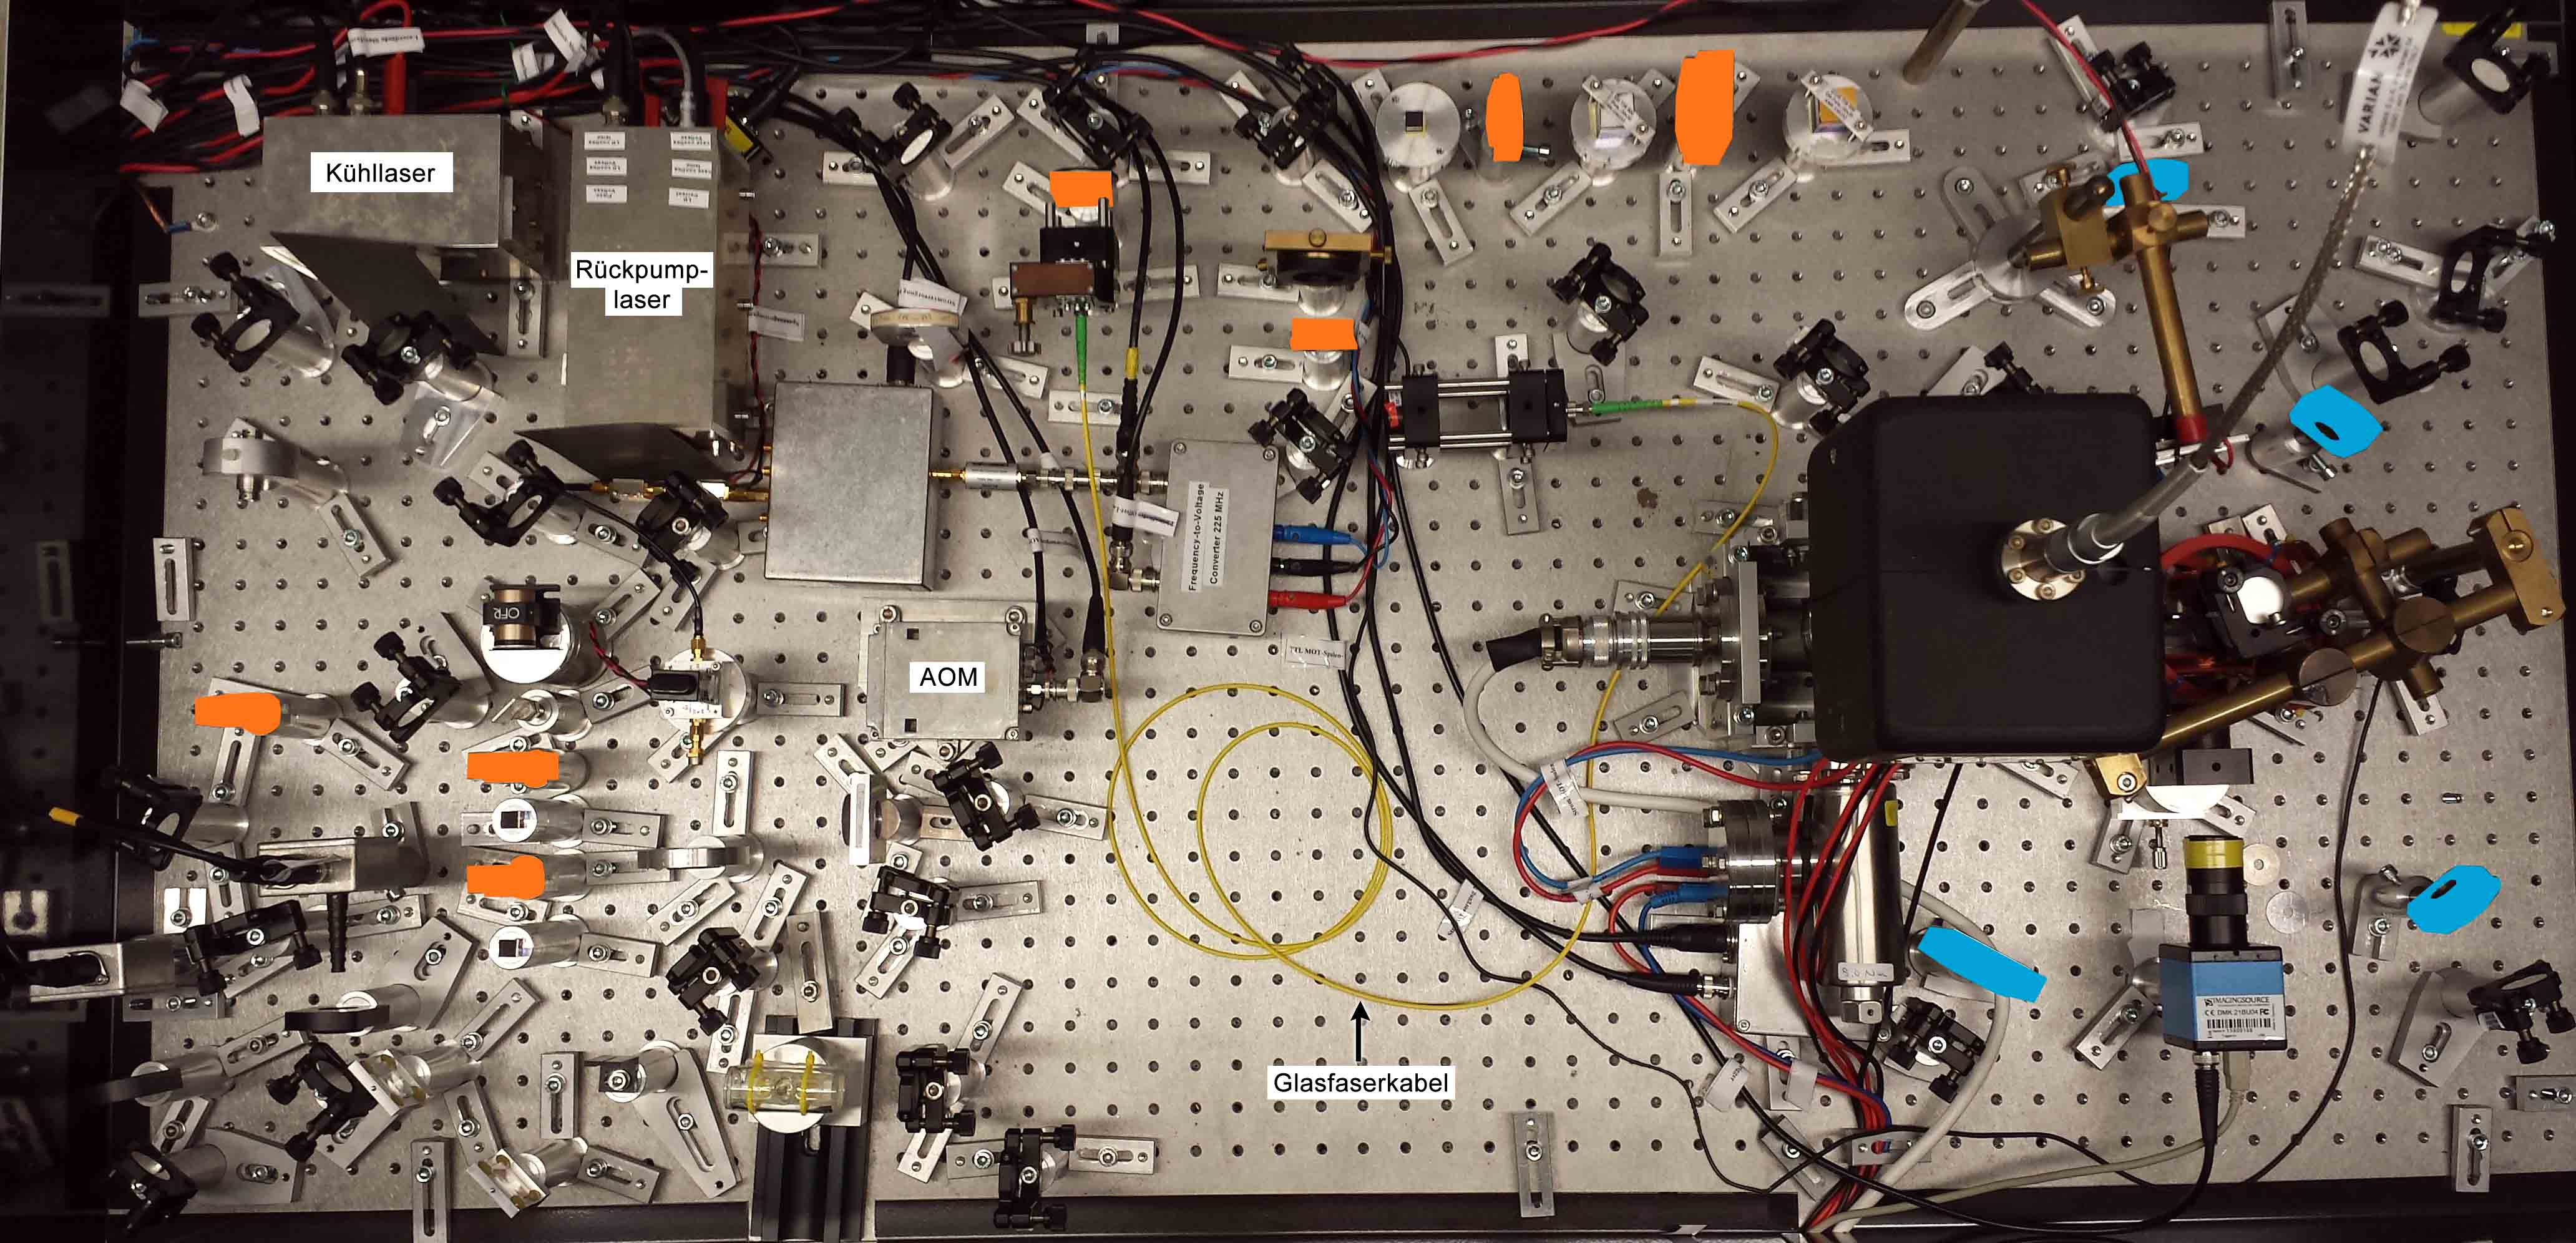
\includegraphics[width=480px]{Bilder/LHLV.jpg}
						\caption{\textcolor[cmyk]{0,0.68,0.98,0}{$\lambda/2$}- und \textcolor[cmyk]{0.75,0.19,0.03,0}{$\lambda/4$}-Platten}
						\label{fig:LH}
					\end{figure}
					
					\begin{figure}[htb!]
						\centering
						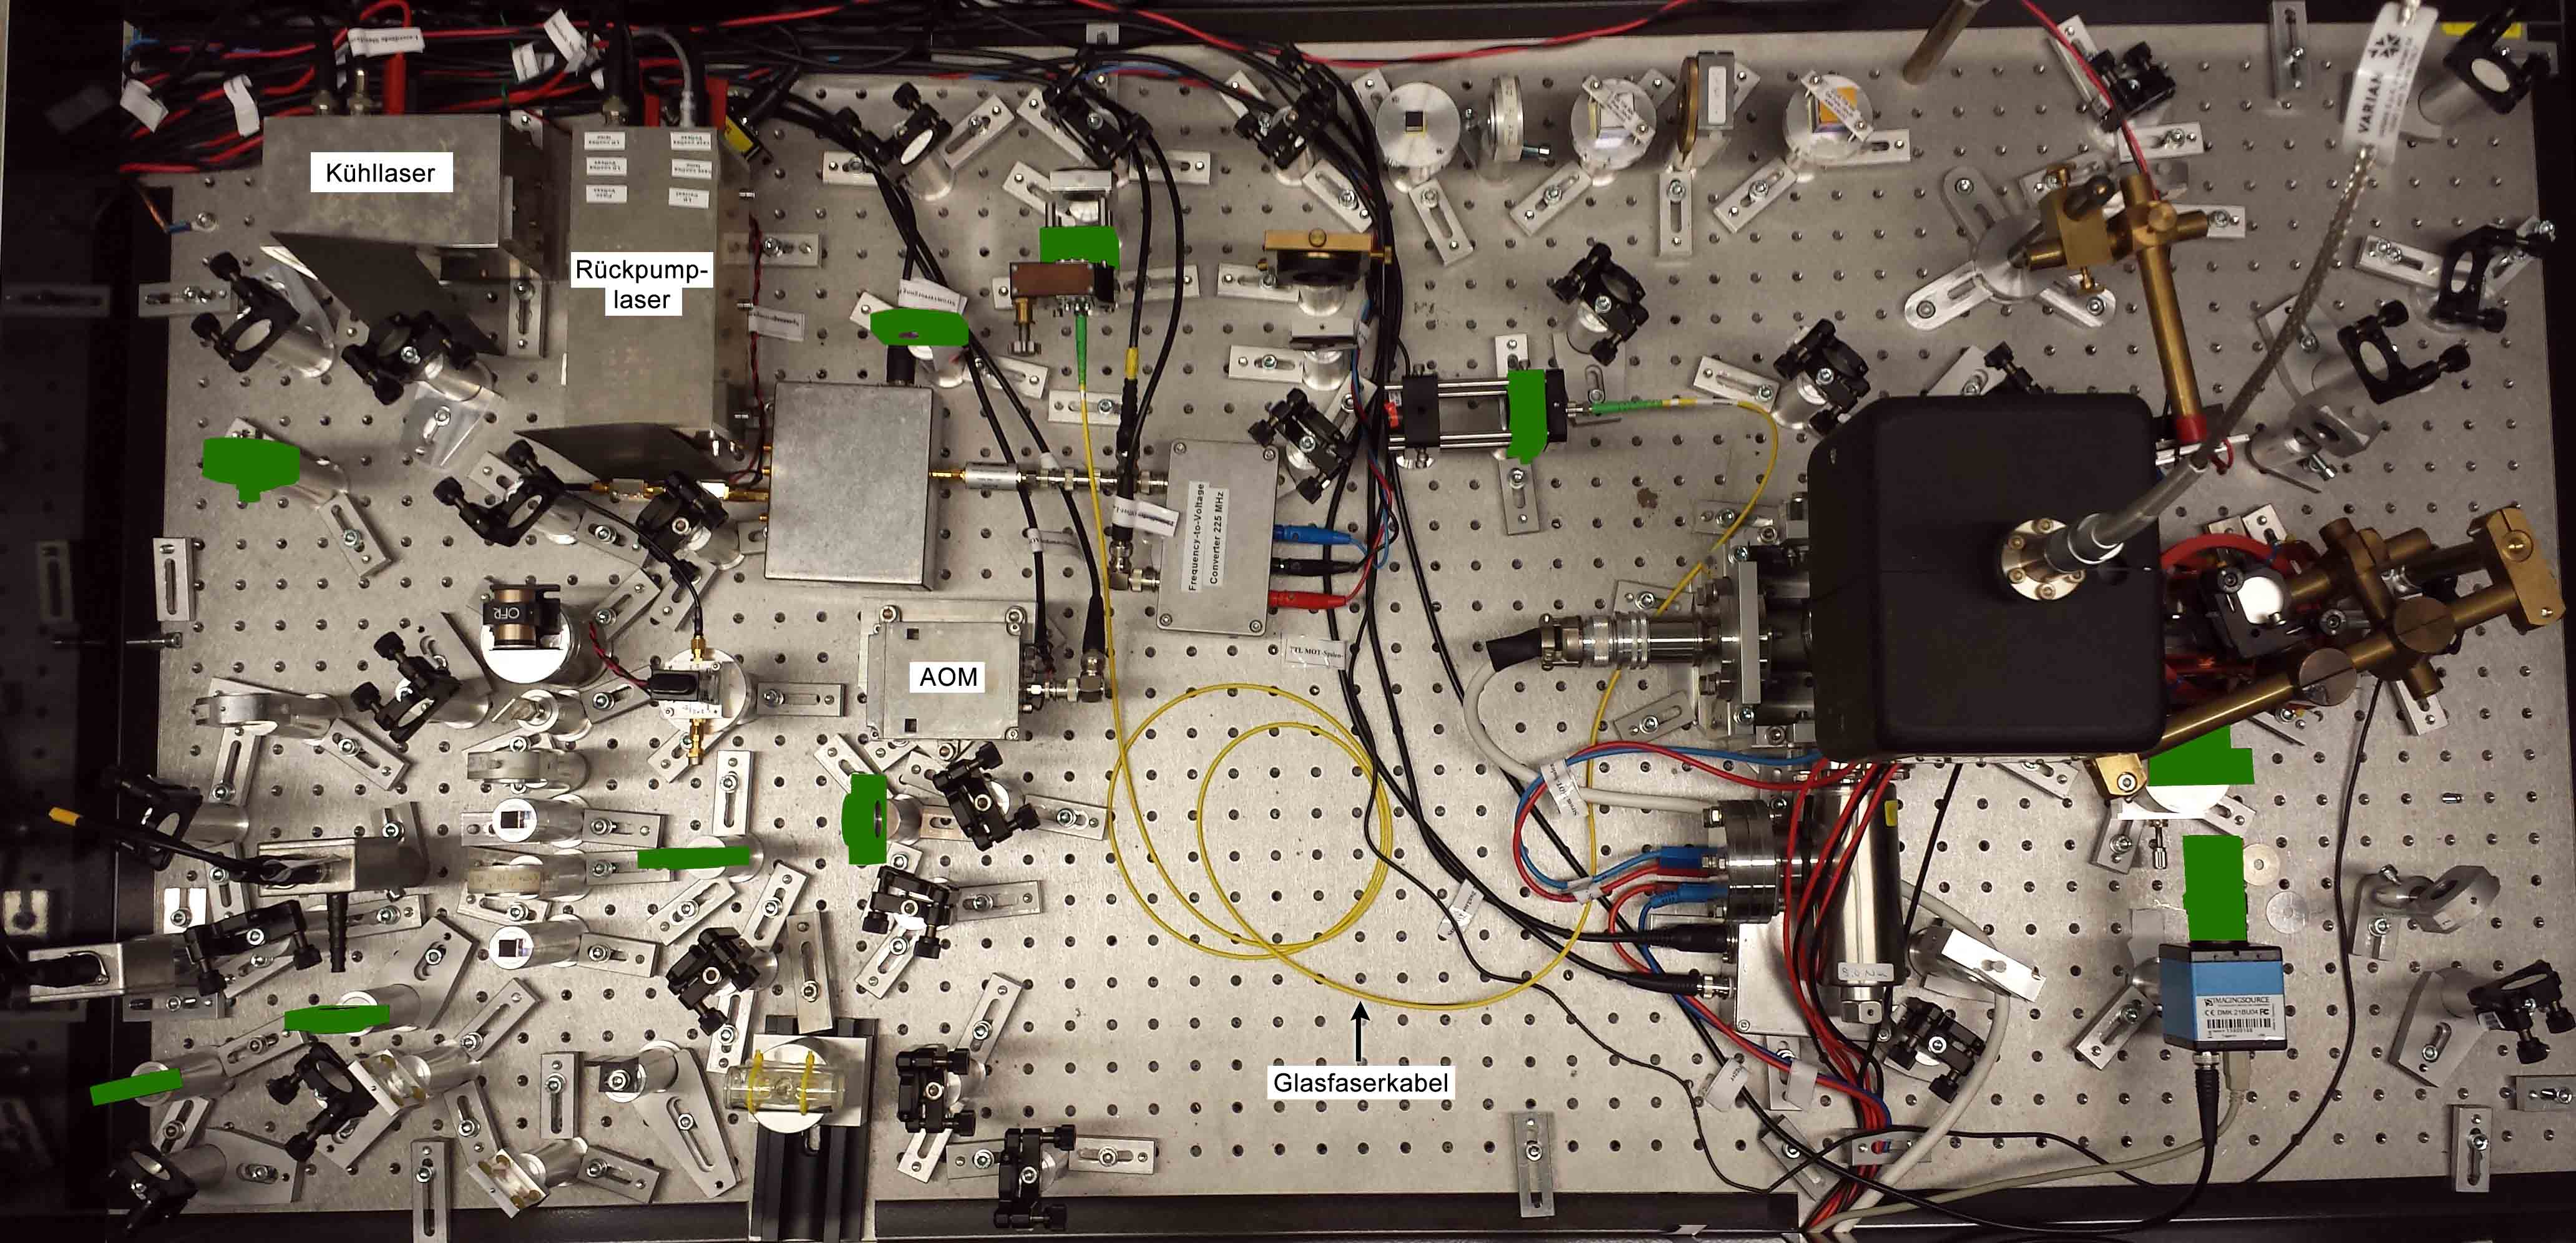
\includegraphics[width=480px]{Bilder/LN.jpg}
						\caption{\textcolor[cmyk]{0.84,0.30,1,0.2}{Linsen}}
						\label{fig:LI}
					\end{figure}
					
					\begin{figure}[htb!]
						\centering
						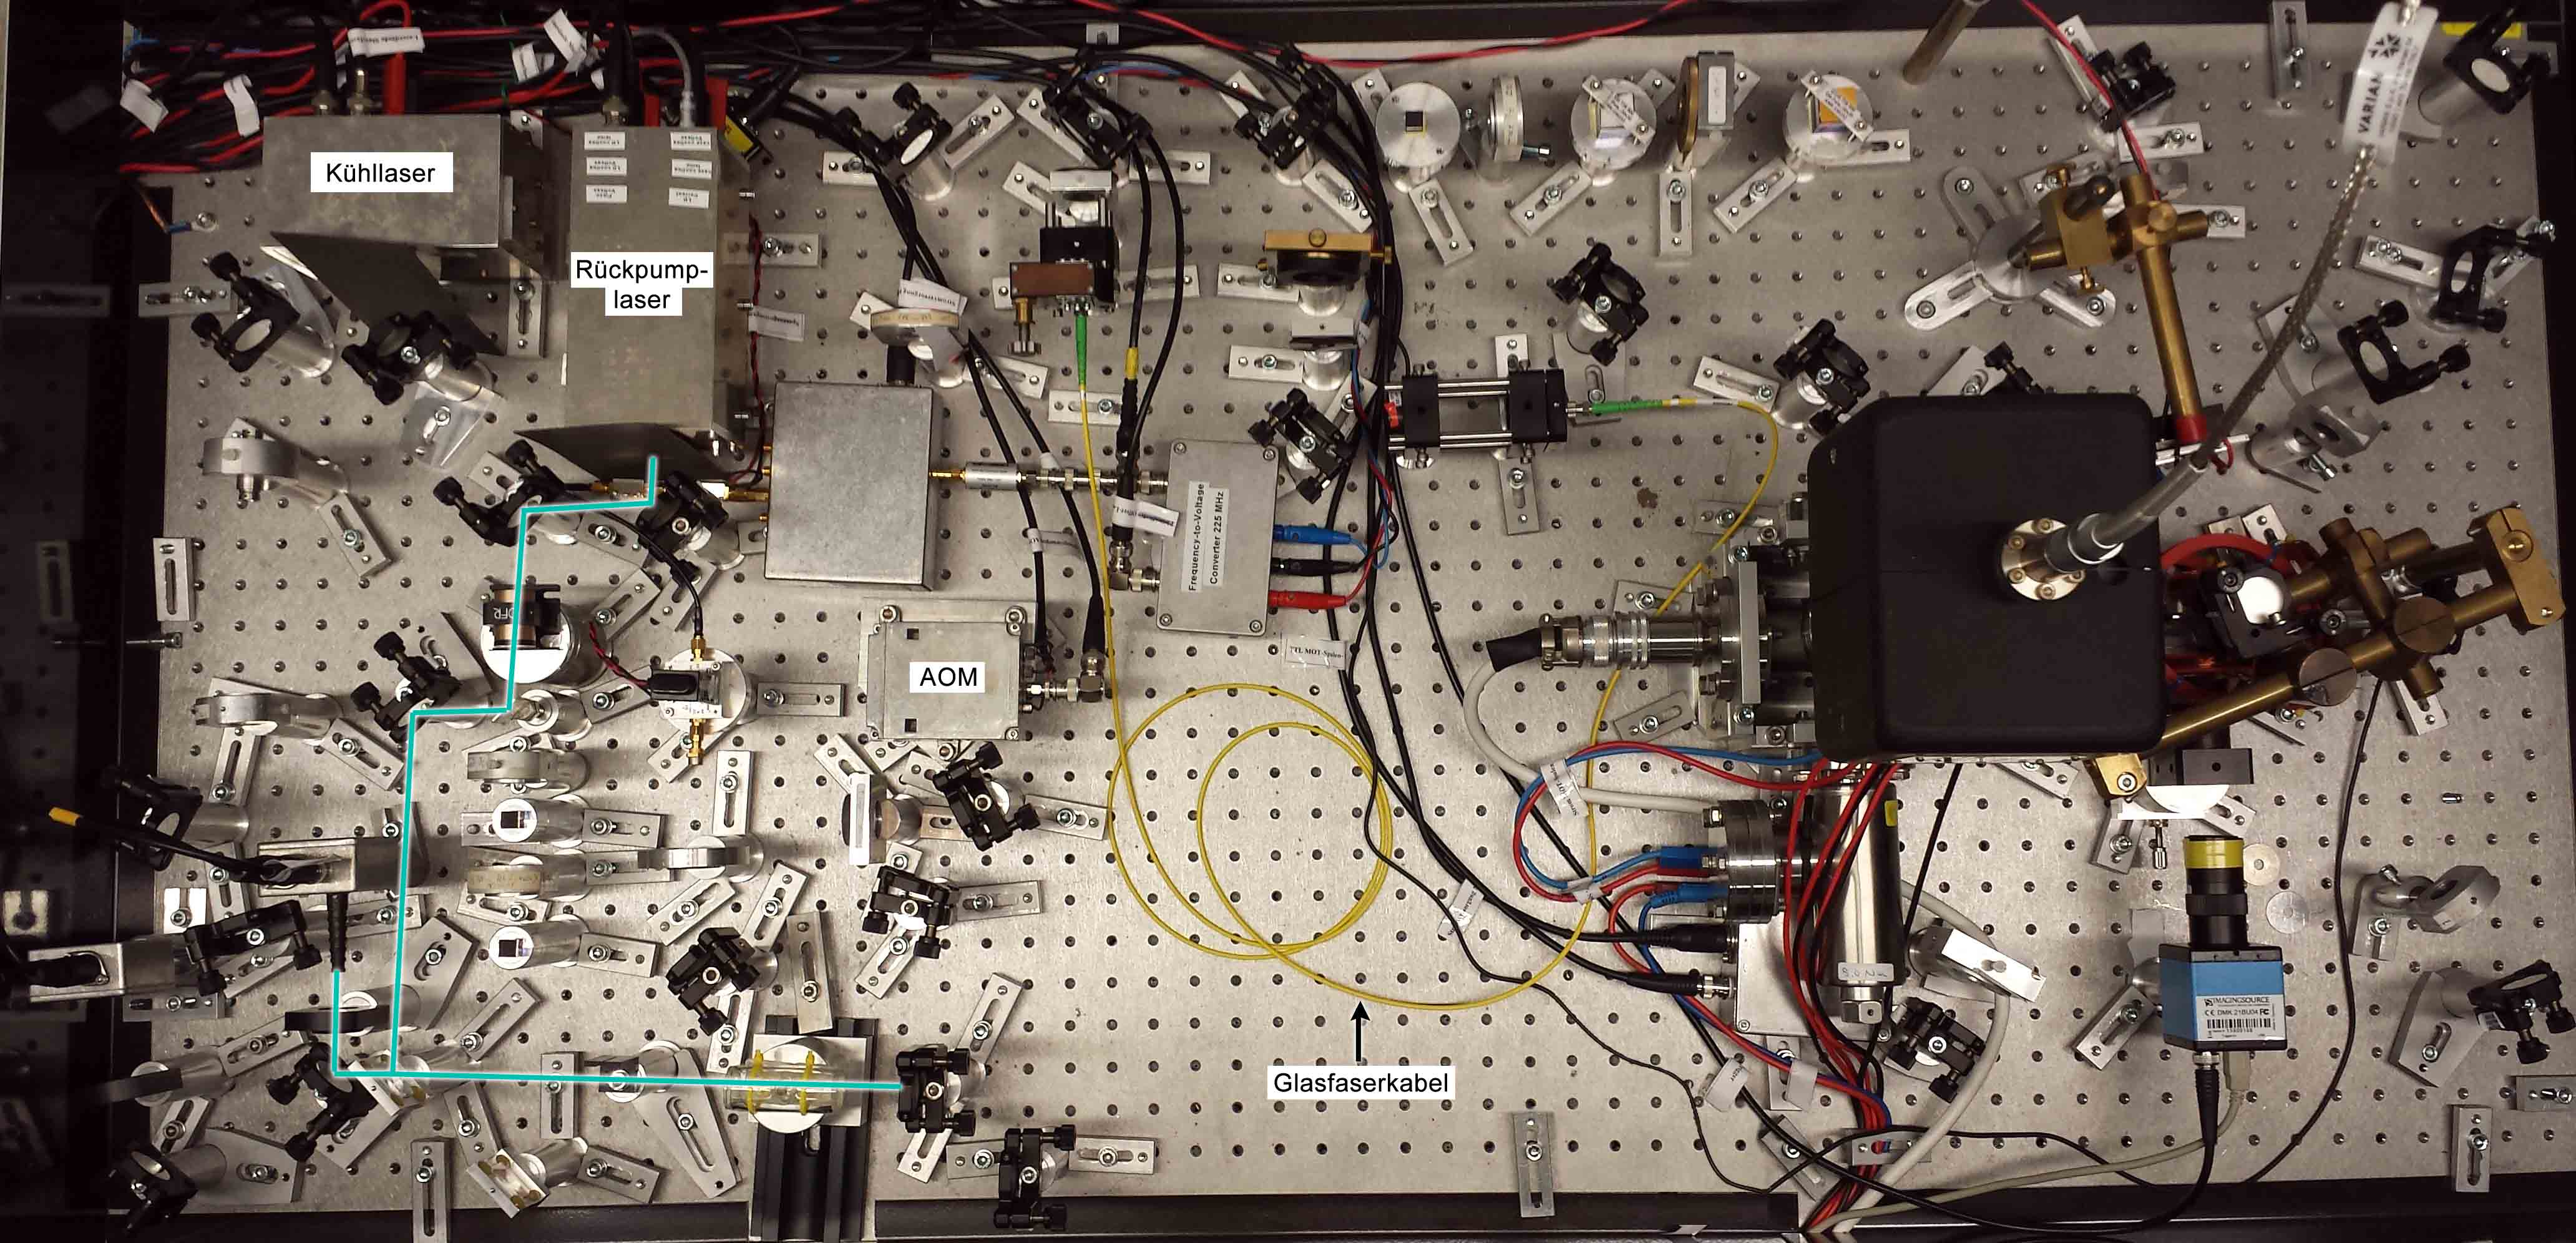
\includegraphics[width=480px]{Bilder/SPM.jpg}
						\caption{Strahlengang für die \textcolor[cmyk]{0.71,0,0.4,0}{Spektroskopie des Rückpumplasers}}
						\label{fig:SPM}
					\end{figure}
					
					\begin{figure}[htb!]
						\centering
						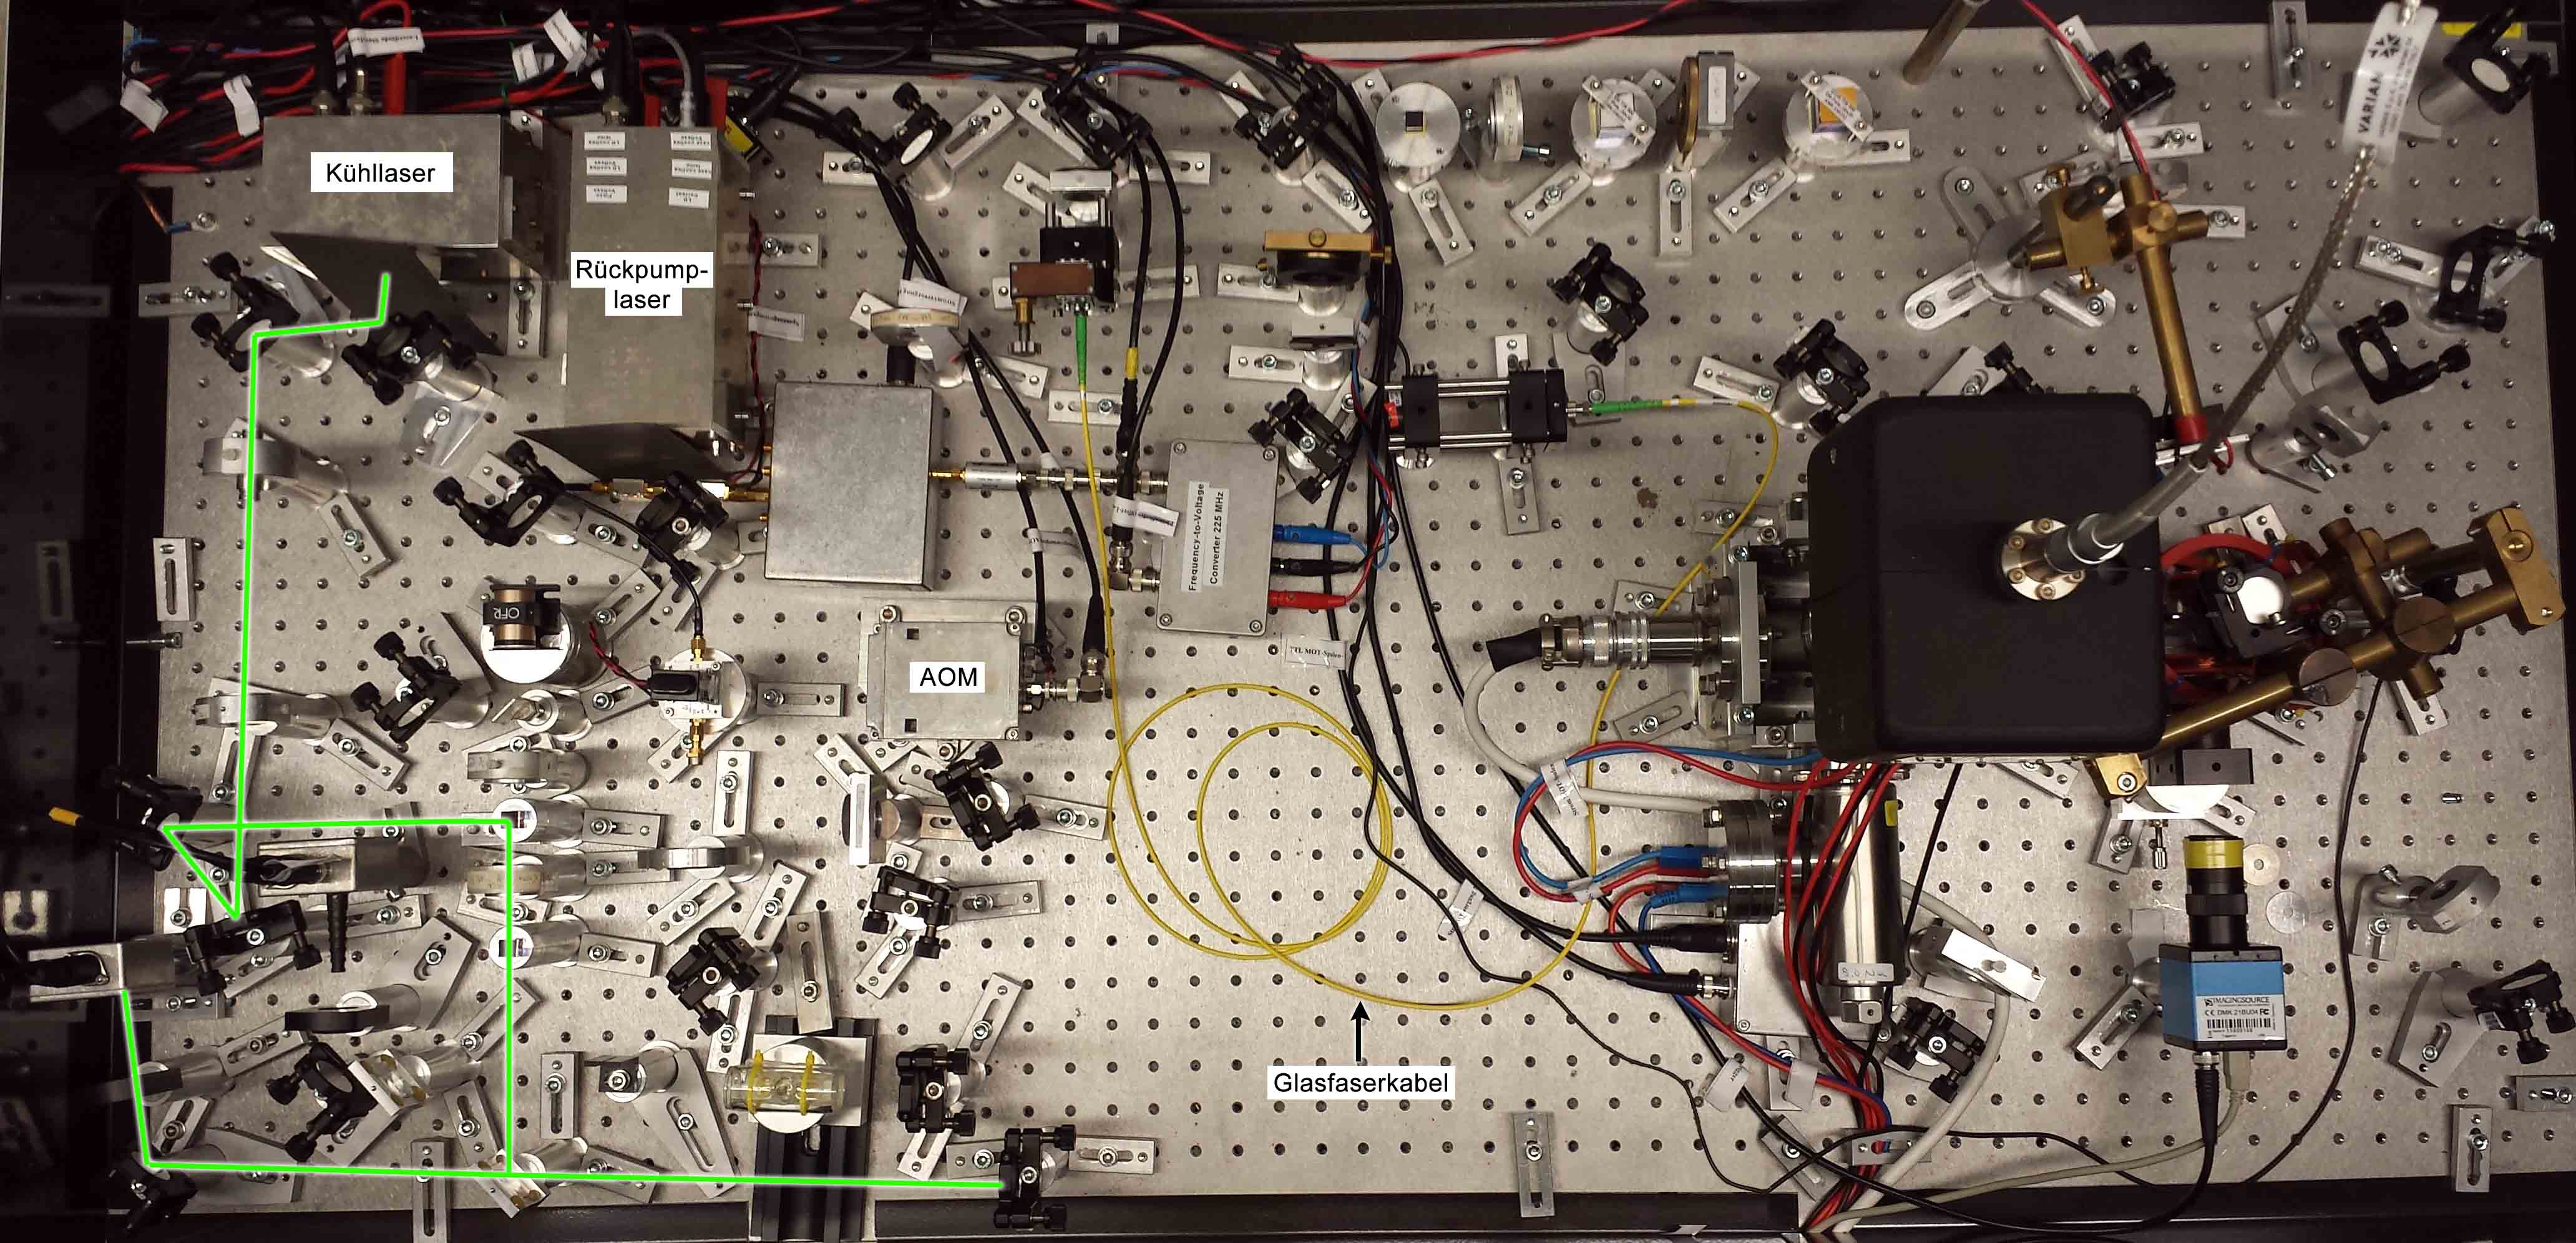
\includegraphics[width=480px]{Bilder/SPS.jpg}
						\caption{Strahlengang für die \textcolor[cmyk]{0.6,0,1,0}{Spektroskopie des Kühllasers}}
						\label{fig:SPS}
					\end{figure}
					
					\begin{figure}[htb!]
						\centering
						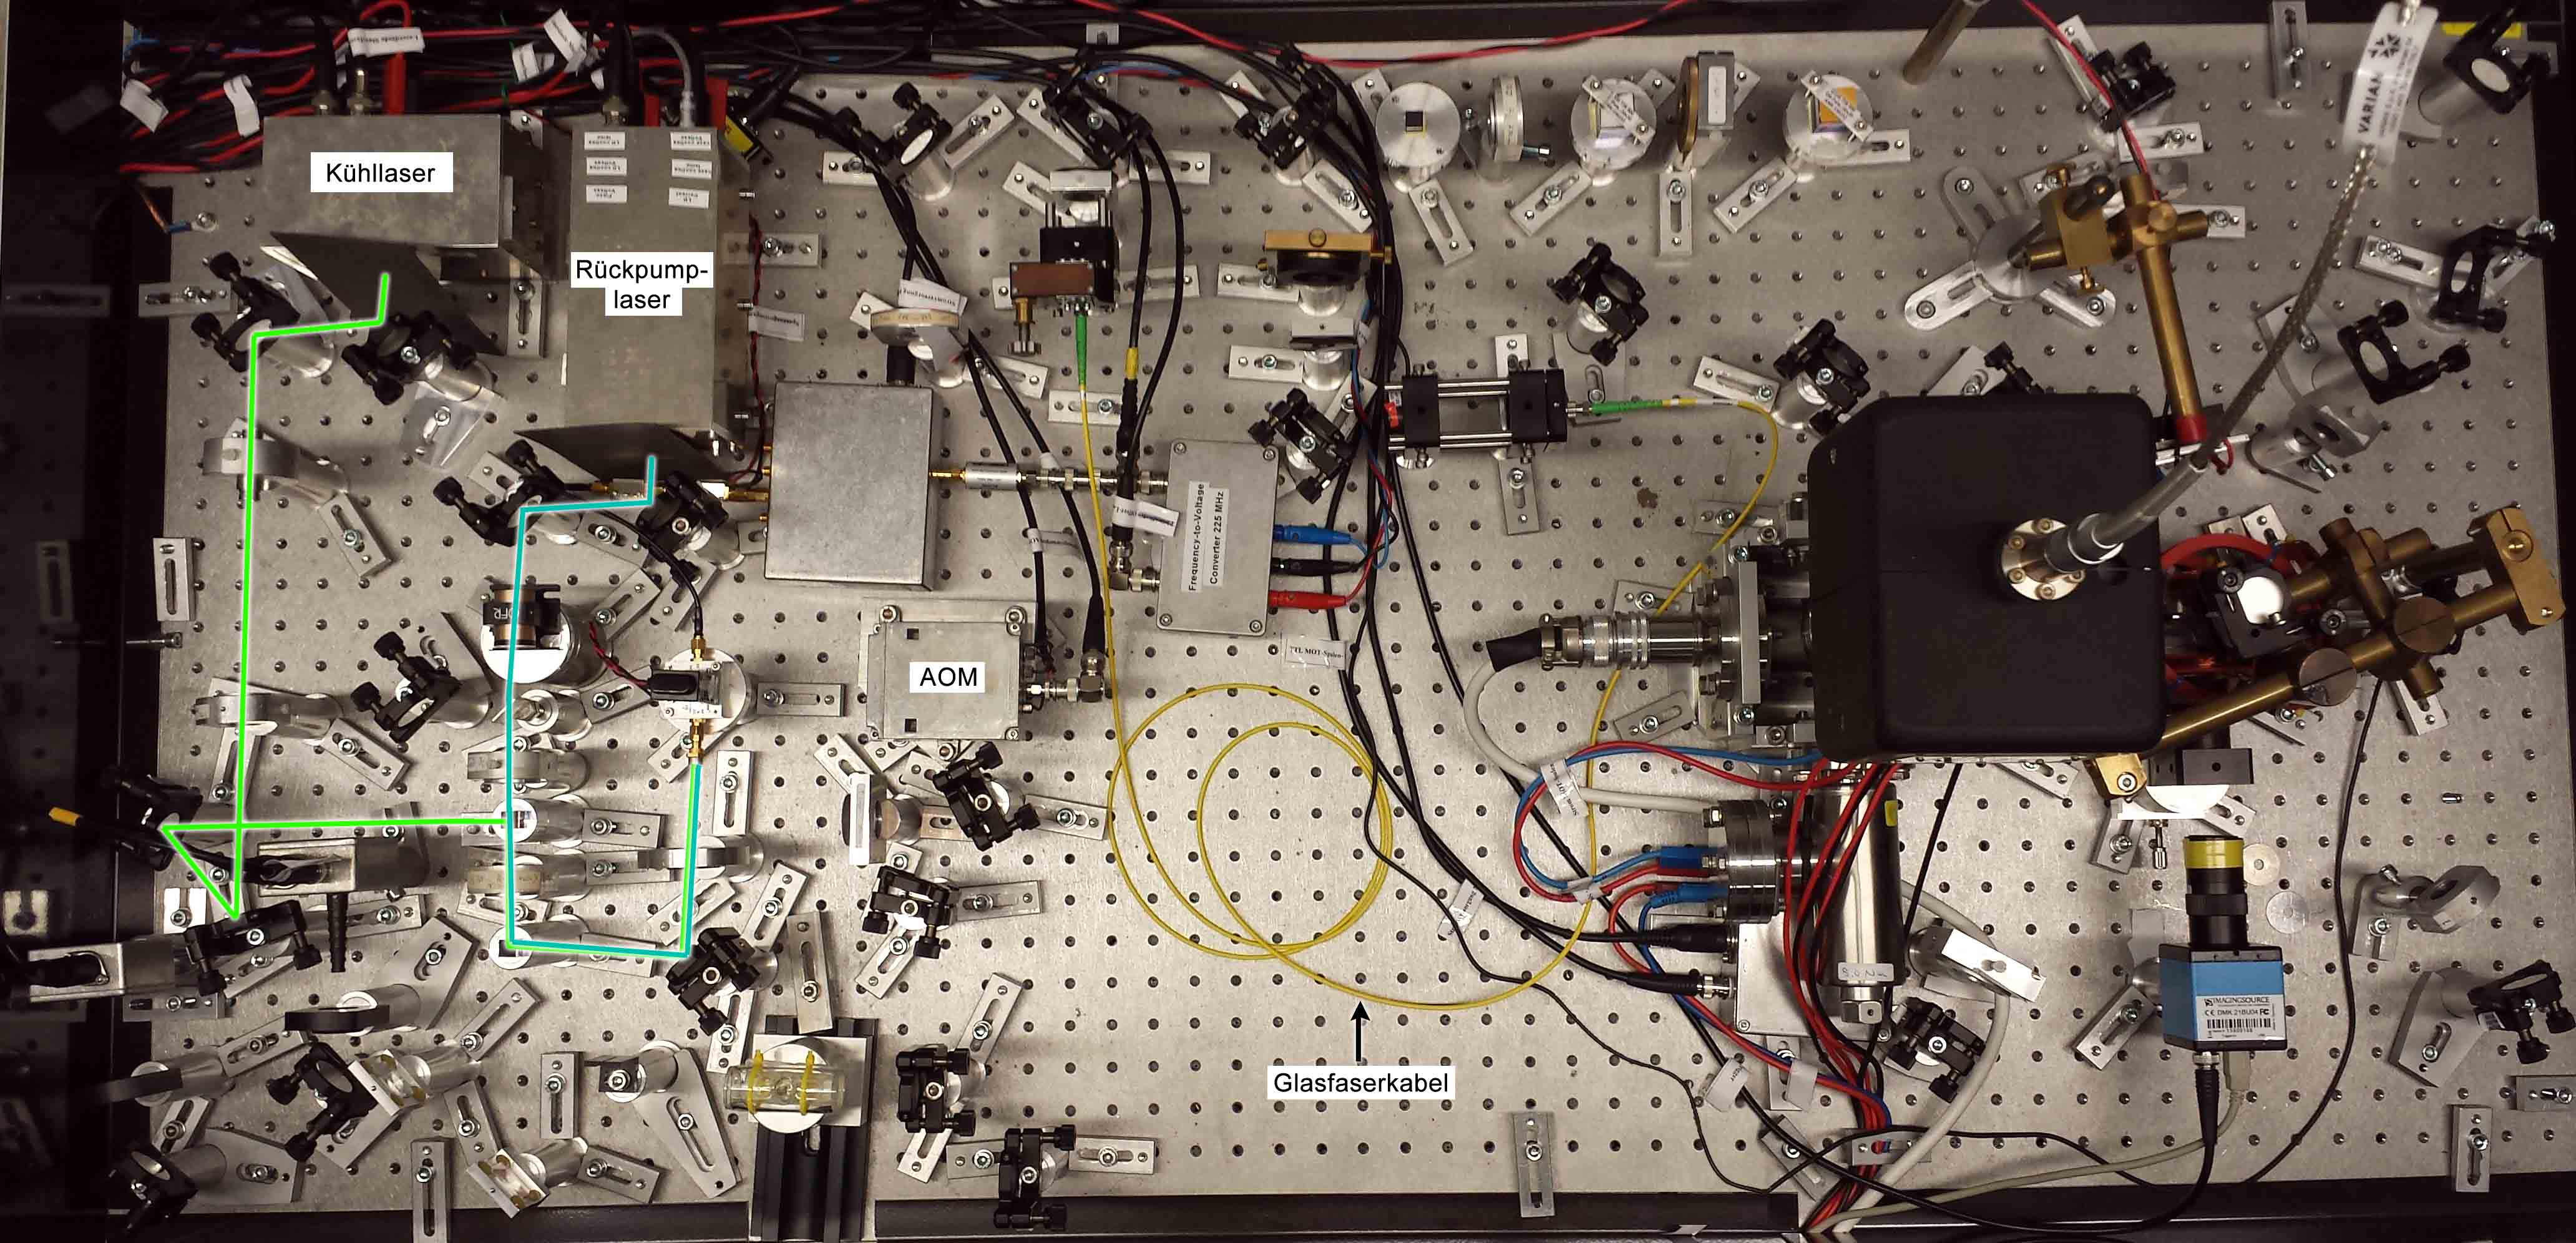
\includegraphics[width=480px]{Bilder/OFL.jpg}
						\caption{Strahlengang für den Offsetlock des Kühllasers}
						\label{fig:OFL}
					\end{figure}
					
					\begin{figure}[htb!]
						\centering
						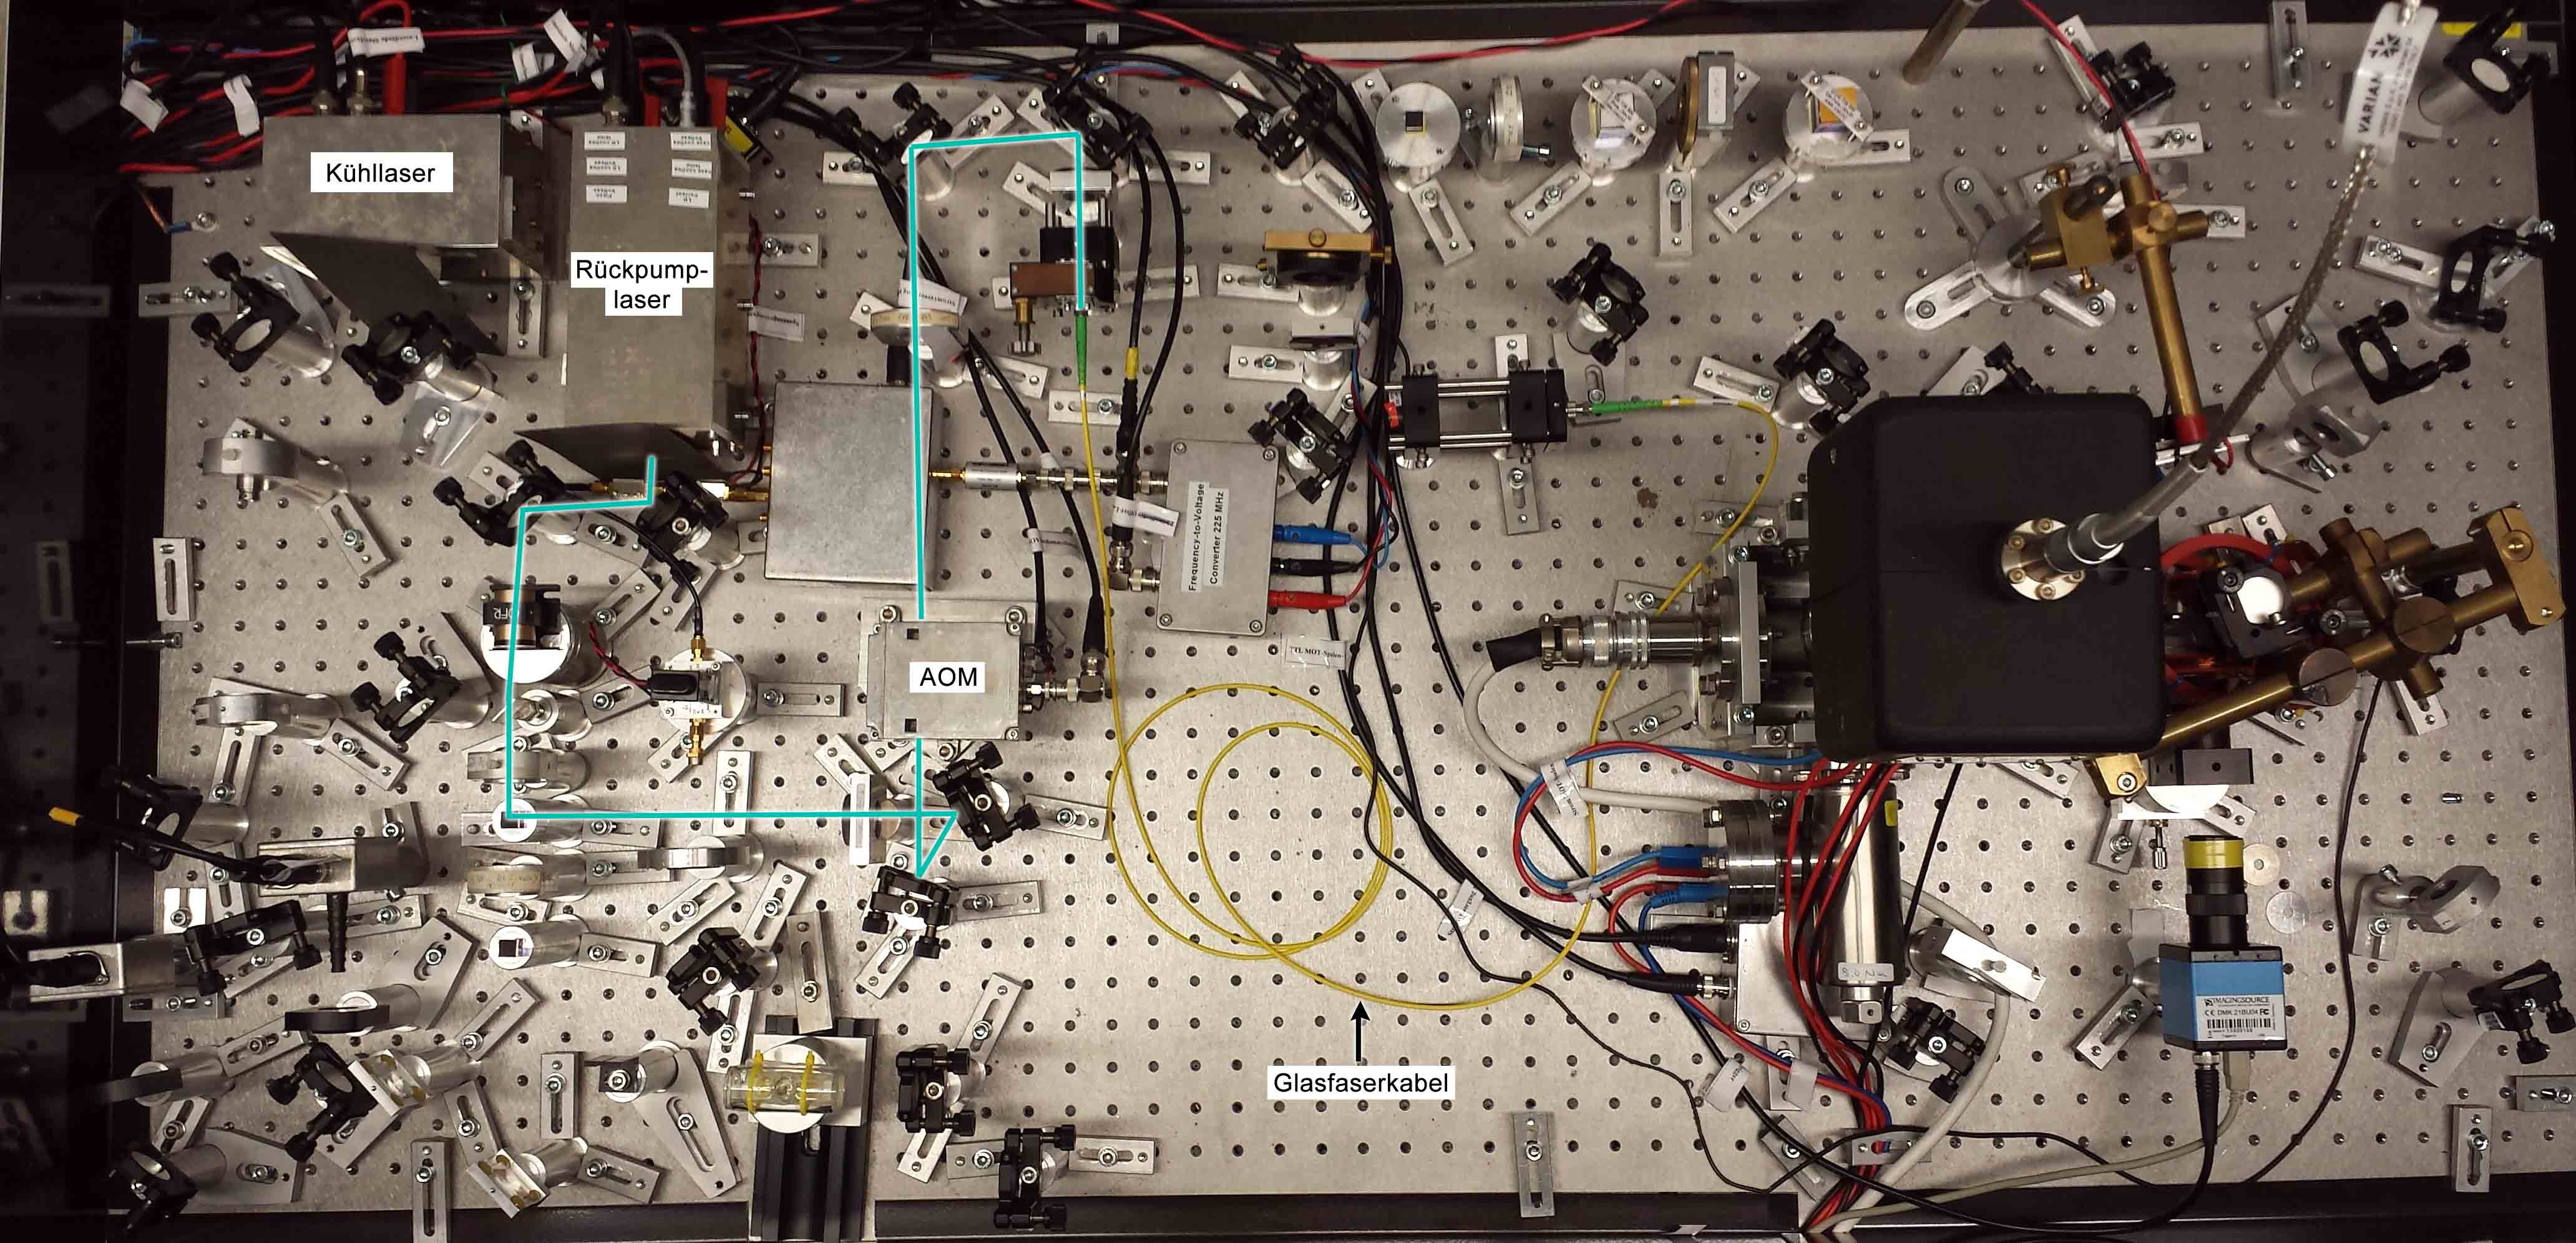
\includegraphics[width=480px]{Bilder/MM.jpg}
						\caption{Strahlengang des \textcolor[cmyk]{0.71,0,0.4,0}{Rückpumplichtes zum Glasfaserkabel} für die MOT}
						\label{fig:MM}
					\end{figure}
					
					\begin{figure}[htb!]
						\centering
						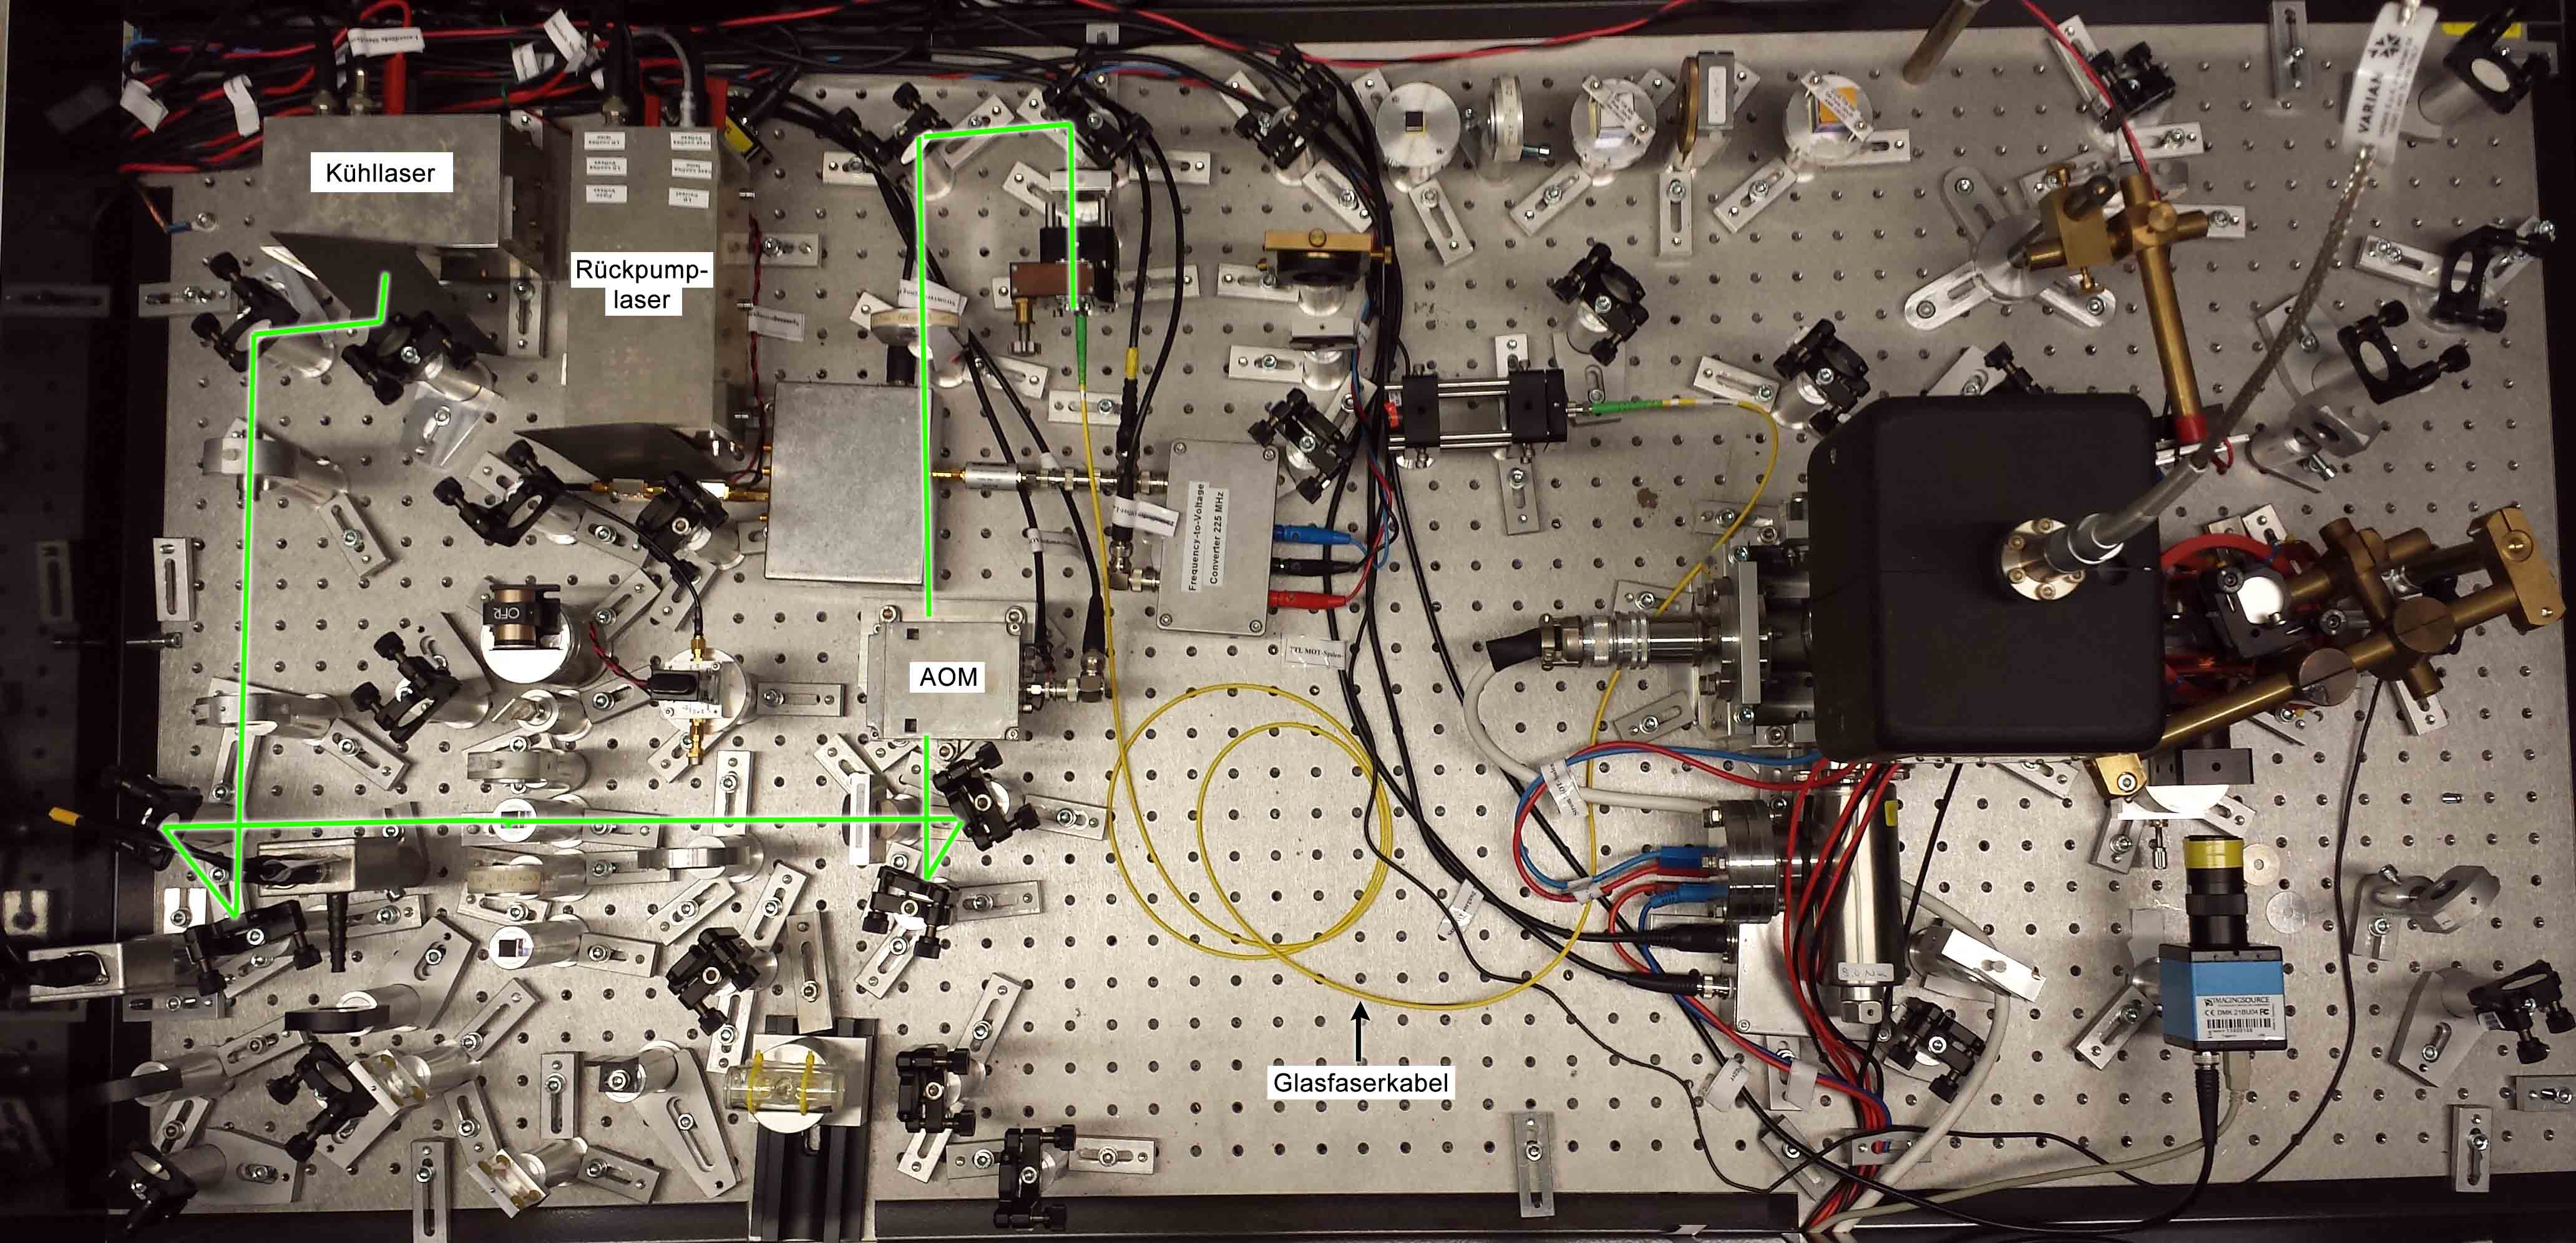
\includegraphics[width=480px]{Bilder/SZM.jpg}
						\caption{Strahlengang des  \textcolor[cmyk]{0.6,0,1,0}{Kühllichtes zum Glasfaserkabel} für die MOT}
						\label{fig:SZM}
					\end{figure}
					
					\clearpage
					
					~\\
					
					\begin{figure}[htb!]
						\centering
						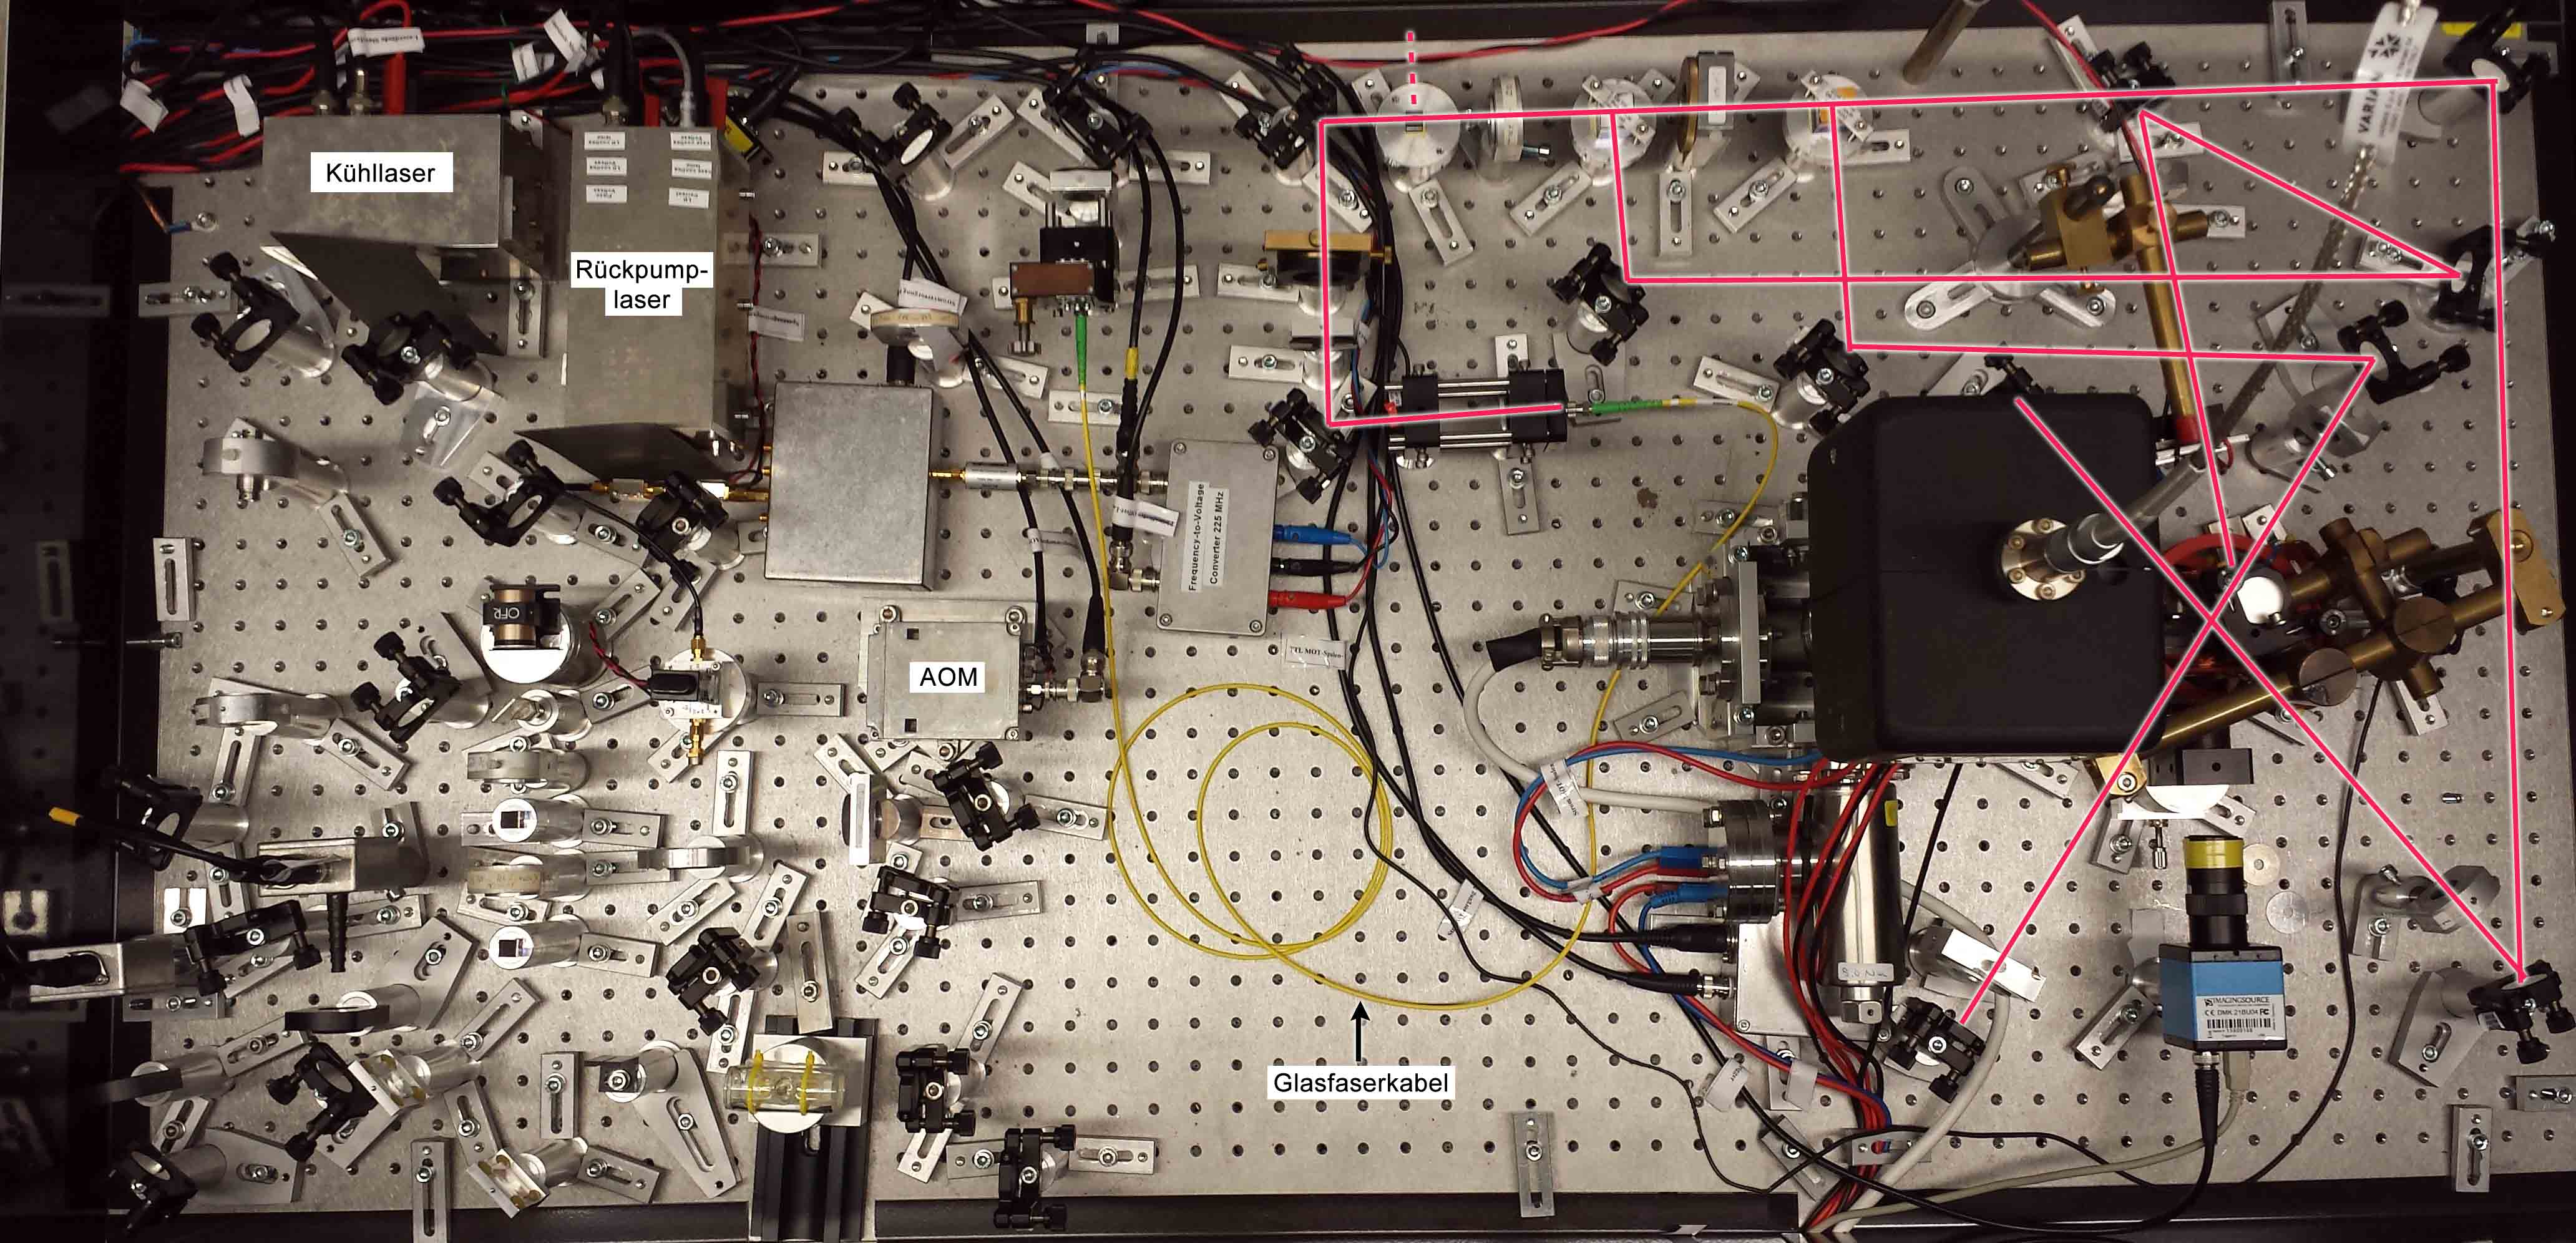
\includegraphics[width=480px]{Bilder/MOTSTG.jpg}
						\caption{Strahlengang \textcolor[cmyk]{0,0.96,0.55,0}{der MOT} nach dem Glasfaserkabel}
						\label{fig:MOTSTG}
					\end{figure}
					
					~\\
					~\\
					~\\
					
					\begin{figure}[htb!]
						\centering
						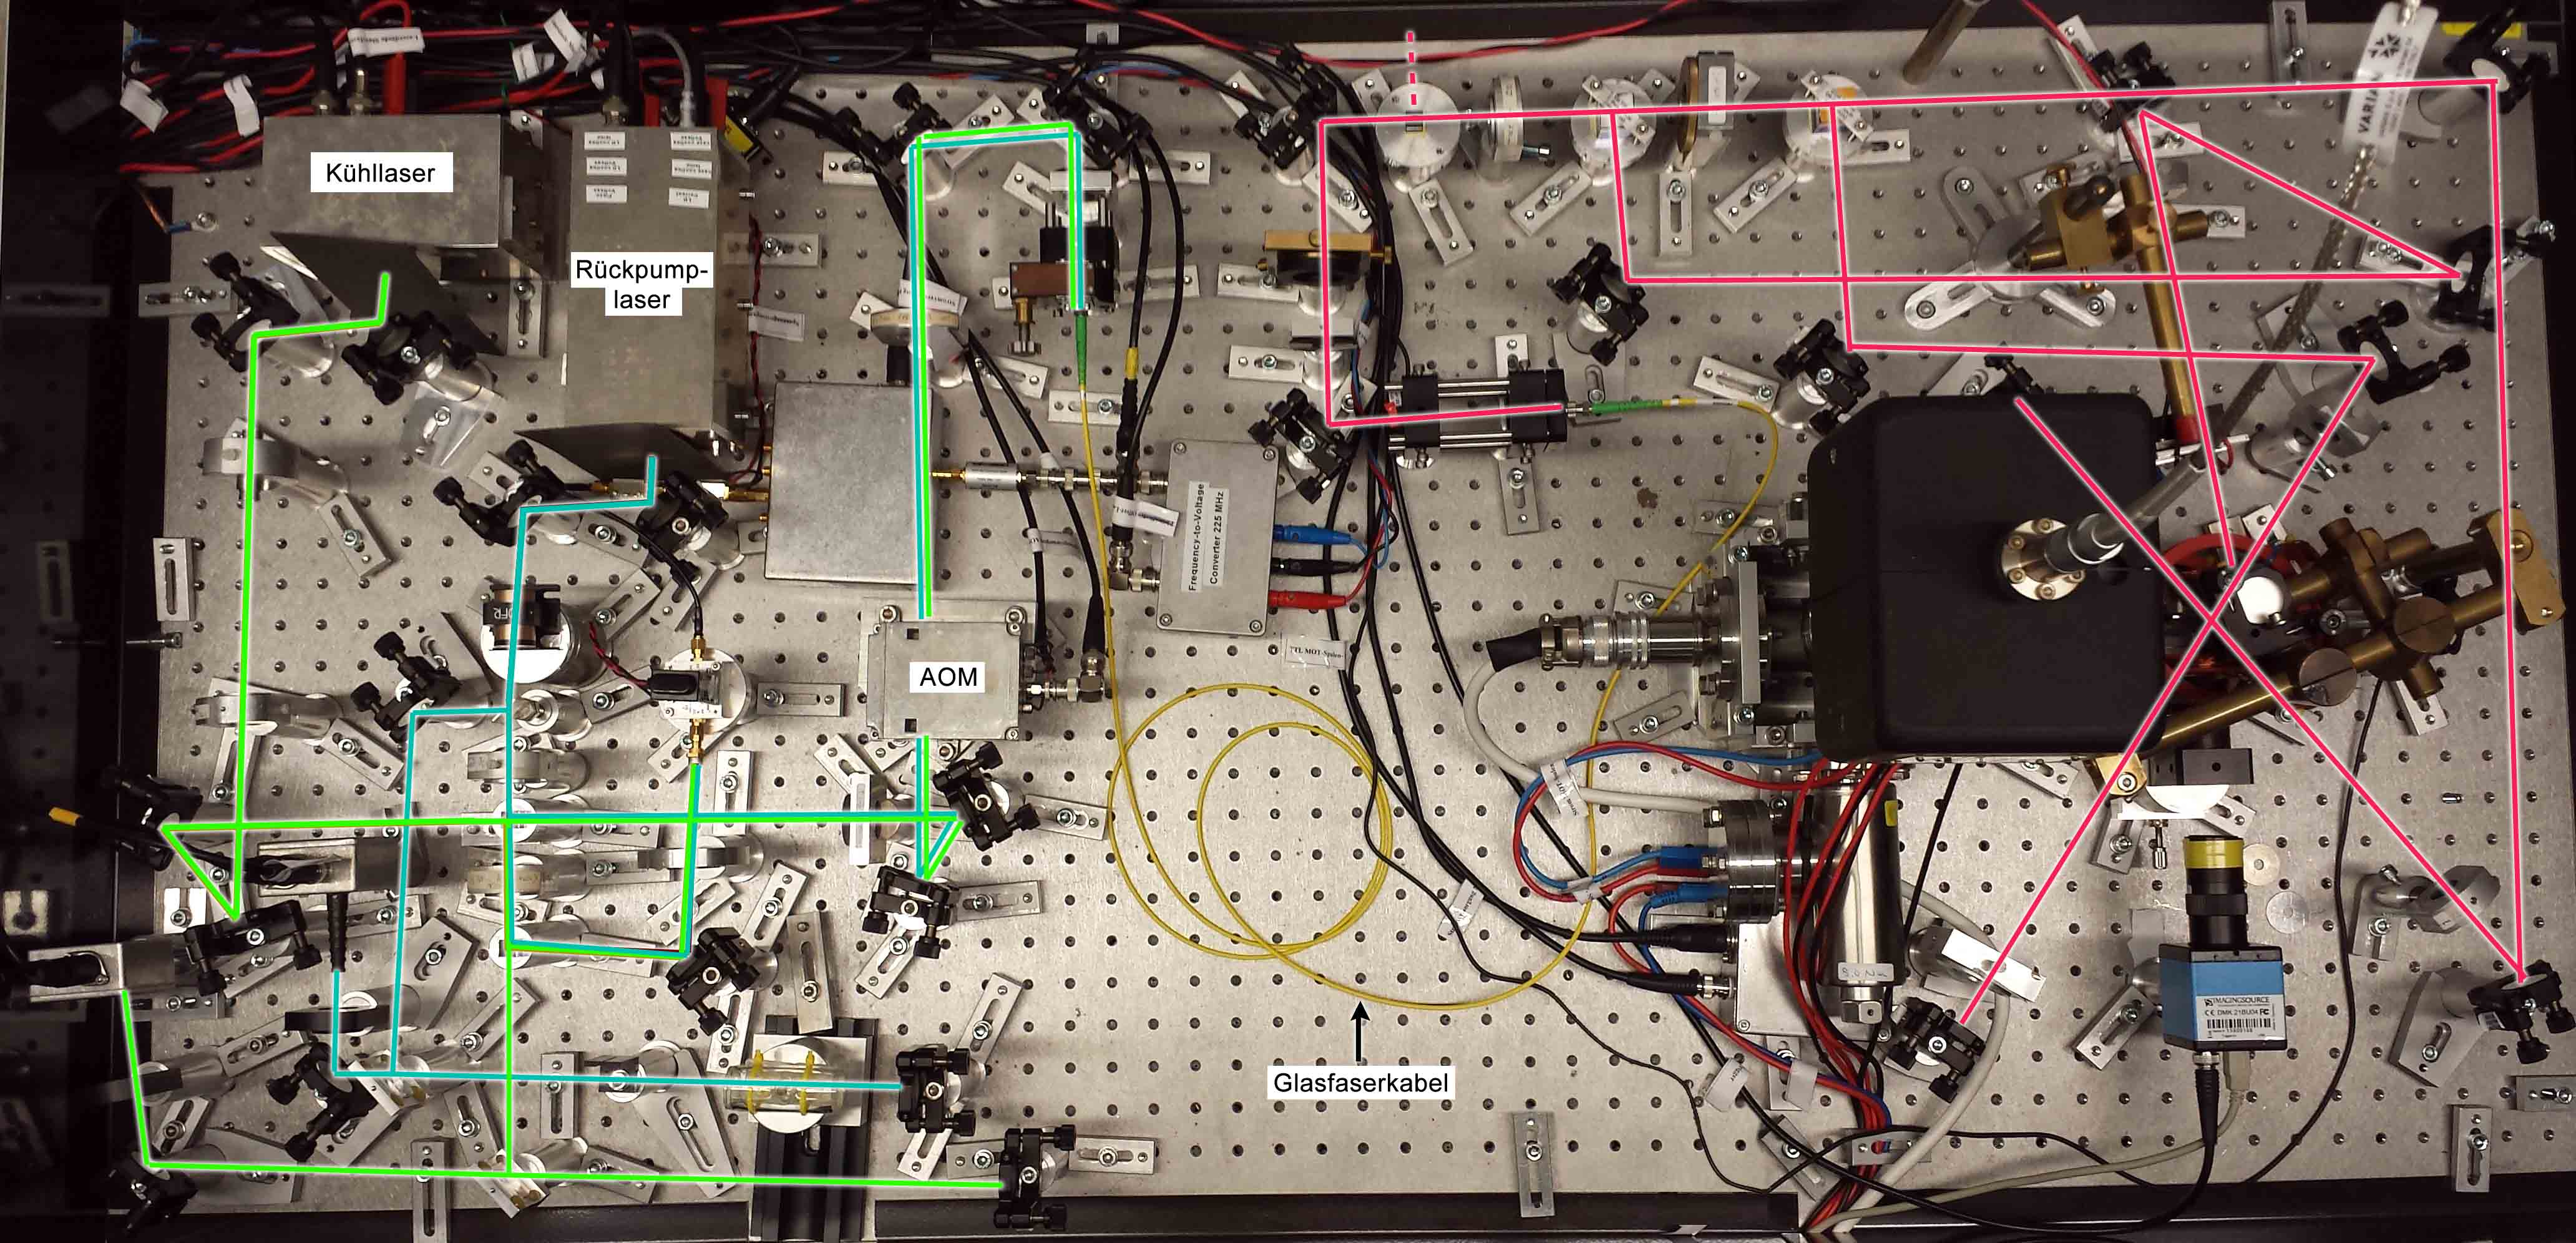
\includegraphics[width=480px]{Bilder/STGK.jpg}
						\caption{alle Strahlengänge}
						\label{fig:STGK}
					\end{figure}
					
					\begin{figure}
						\centering
						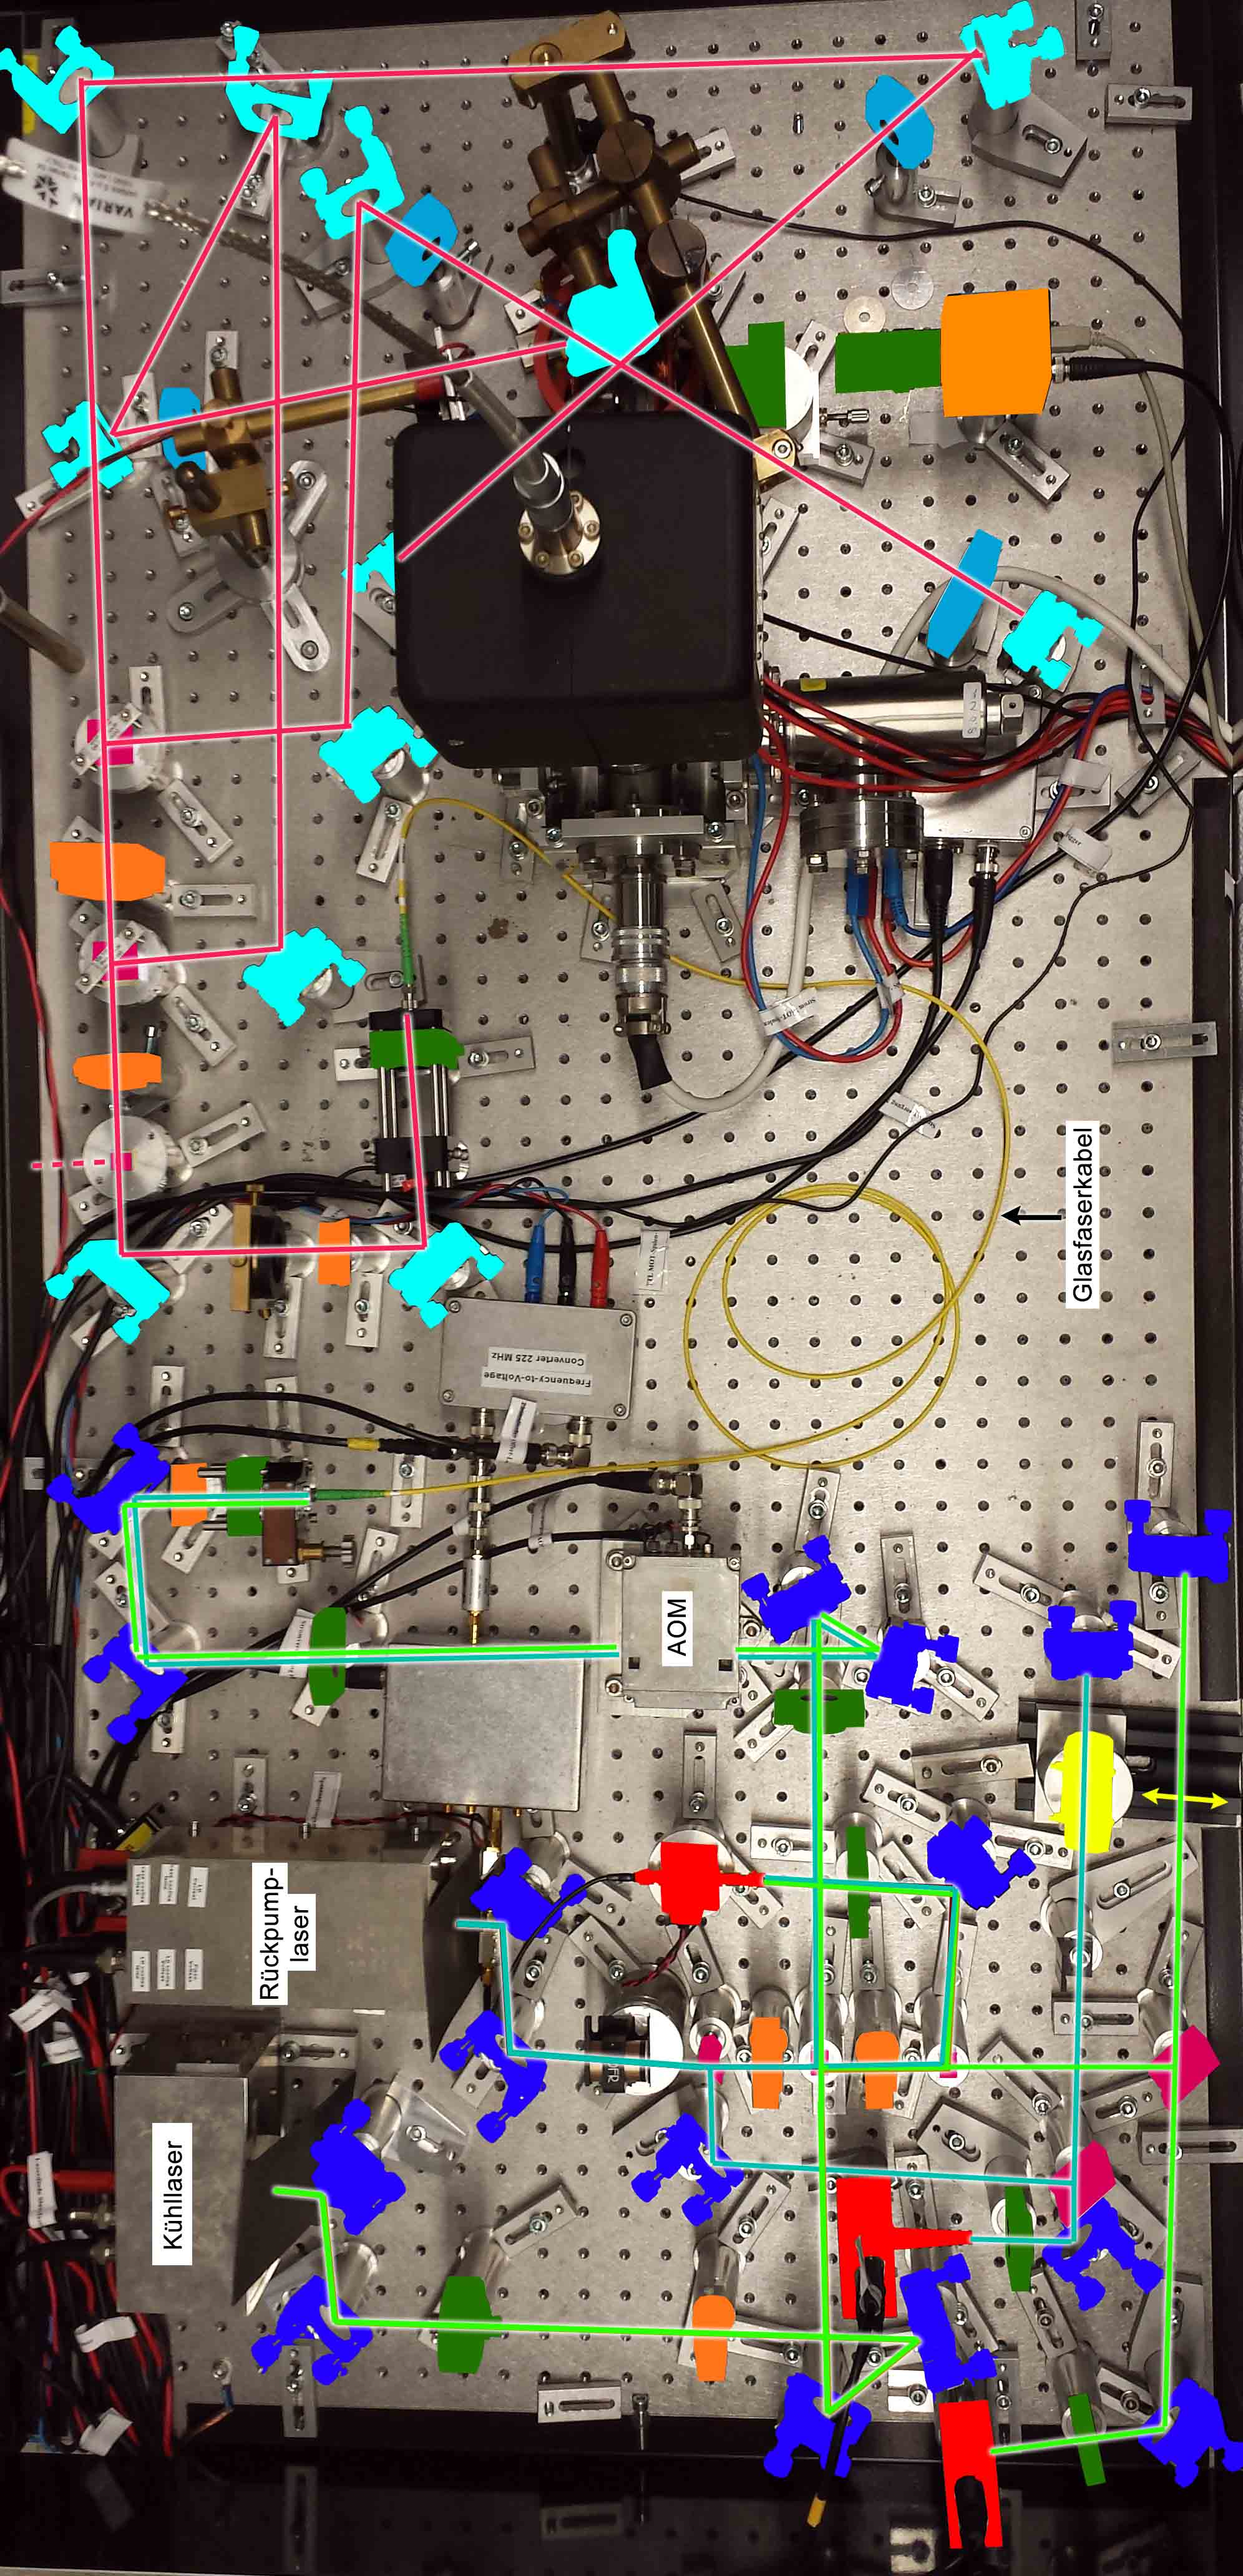
\includegraphics[width=320px]{Bilder/AEGBg.jpg}
						\caption{alle Strahlengänge und alle Elemente}
						\label{fig:AEGB}
					\end{figure}
					

\newpage

%	\appendix
%	\newpage
%	\nocite{*}
%\printbibheading[title = {Literaturverzeichnis}]
%\printbibliography[keyword=bild,heading=subbibliography,title={Bildquellen}]%
%\printbibliography[keyword=lit,heading=subbibliography,title={Literatur}]
%\printbibliography[keyword=erg,heading=subbibliography,title={Ergänzende Literatur}]
Internetquellen letztmalig im März 2023 aufgerufen

%	\renewcommand{\bibname}{Wesentliche Literatur}
%	\bibliographystyleq{osa_mod}	
%	\bibliographyq{mybib}	
%	\bibliographystylewes{osa_mod}	
%	\bibliographywes{mybib}
%	\bibliographystyleerg{osa_mod}	
%	\bibliographyerg{mybib}

%	\cleardoublepage
	
\newpage
\subsection*{Wichtige Punkte zum Laserschutz}
Ganz allgemein gilt: \textbf{Im Umgang mit Lasern ist der gesunde Menschenverstand nicht zu ersetzen!} Einige
spezielle Hinweise werden im folgenden angeführt.
\begin{enumerate}
\item Die Laserschutzvorschriften sind \textbf{immer} zu beachten.
\vspace{-2pt}
\item Kopf \textbf{niemals} auf Strahlhöhe.
\vspace{-2pt}
\item Richtige Schutzbrille aufsetzen; Wellenlänge und Leistung müssen bei der Wahl berücksichtigt werden. Bitte beim Betreuer oder Laserschutzbeauftragten, oder an den Aushängen an den Labortüren informieren!
\vspace{-2pt}
\item Achtung: praktisch alle Laser für Laboranwendungen sind mindestens Klasse 3, also von vornherein für die Augen gefährlich, ggf. auch für die Haut -- evtl. auch hierfür Schutzmaßnahmen ergreifen.
\vspace{-2pt}
\item Zur Justage kann der Laserstrahl mittels Wandlerkarten sichtbar gemacht werden. Zu beachten ist: Diese halten keine sehr hohen Leistungen aus und besitzen im allgemeinen eine reflektierende Oberfläche. Achtung deshalb vor \textbf{Reflektionen}! Auch Kameras
besitzen eine \textbf{Zerstörschwelle}!
\vspace{-2pt}
\item Spiegel und sonstige Komponenten nie in den \textbf{ungeblockten} Laserstrahl einbauen! Vor Einbau immer überlegen, in welche Richtung der Reflex geht! Diese Richtung zunächst blocken, bevor der Strahl wieder frei gegeben wird.
\vspace{-2pt}
\item \textbf{Nie mit reflektierenden Werkzeugen im Strahlengang hantieren}! Unkontrollierbare Reflexe! Vorsicht ist z.B. auch mit BNC-Kabeln geboten, die in den Strahlengang gelangen könnten!
Gleiches gilt auch für Uhren und Ringe. Diese vorsichtshalber ausziehen, wenn Sie mit den Händen im Strahlengang arbeiten.
\vspace{-2pt}
\item Auch Leistungsmessgeräte können Reflexe verursachen! Unbeschichtete Silizium-Fotodioden reflektieren über 30\% des Lichtes!
\vspace{-2pt}
\item Achtung im Umgang mit \textbf{Strahlteilerwürfeln}! Diese haben immer einen zweiten Ausgang! Ggf. abblocken!
\vspace{-2pt}
\item \textbf{Warnlampen} bei Betrieb des Lasers anschalten und nach Beendigung der Arbeit wieder ausschalten.
\vspace{-2pt}
\item Dafür sorgen, dass auch Dritte im Labor die richtigen Schutzbrillen tragen, oder sich außerhalb des Laserschutzbereiches befinden.
\vspace{-2pt}
\item Filtergläser in Laserschutzbrillen dürfen \textbf{\textit{grundsätzlich nicht}} aus- oder umgebaut
werden!!!
\vspace{-2pt}
\item In besonderem Maße auf Beistehende achten.
\end{enumerate}
Hiermit erkläre ich, dass ich die vorstehenden Punkte gelesen und verstanden habe. Ich bestätige, dass ich eine Einführung in den Umgang mit Lasern sowie eine arbeitsplatzbezogene Unterweisung erhalten habe.\\

~~\\

\begin{tabular}{ll}
 Name:~~~~~~~~~~~~~~~~~~~~~~~~~~~~~~~~~~~~~~~~~~~~~~~~~~~~~~~~~~~ & Arbeitsgruppe:\\
    Unterschrift: & Datum:
\end{tabular}	
\end{document}
